% Options for packages loaded elsewhere
\PassOptionsToPackage{unicode}{hyperref}
\PassOptionsToPackage{hyphens}{url}
\PassOptionsToPackage{space}{xeCJK}
\documentclass[
  a4paper,
]{article}
\usepackage{xcolor}
\usepackage[margin=24mm]{geometry}
\usepackage{amsmath,amssymb}
\setcounter{secnumdepth}{-\maxdimen} % remove section numbering
\usepackage{iftex}
\ifPDFTeX
  \usepackage[T1]{fontenc}
  \usepackage[utf8]{inputenc}
  \usepackage{textcomp} % provide euro and other symbols
\else % if luatex or xetex
  \usepackage{unicode-math} % this also loads fontspec
  \defaultfontfeatures{Scale=MatchLowercase}
  \defaultfontfeatures[\rmfamily]{Ligatures=TeX,Scale=1}
\fi
\usepackage{lmodern}
\ifPDFTeX\else
  % xetex/luatex font selection
  \setmonofont[]{DejaVuSansMono.ttf}
  \ifXeTeX
    \usepackage{xeCJK}
    \setCJKmainfont[]{HaranoAjiMincho-Regular.otf}
  \fi
  \ifLuaTeX
    \usepackage[]{luatexja-fontspec}
    \setmainjfont[]{HaranoAjiMincho-Regular.otf}
  \fi
\fi
% Use upquote if available, for straight quotes in verbatim environments
\IfFileExists{upquote.sty}{\usepackage{upquote}}{}
\IfFileExists{microtype.sty}{% use microtype if available
  \usepackage[]{microtype}
  \UseMicrotypeSet[protrusion]{basicmath} % disable protrusion for tt fonts
}{}
\makeatletter
\@ifundefined{KOMAClassName}{% if non-KOMA class
  \IfFileExists{parskip.sty}{%
    \usepackage{parskip}
  }{% else
    \setlength{\parindent}{0pt}
    \setlength{\parskip}{6pt plus 2pt minus 1pt}}
}{% if KOMA class
  \KOMAoptions{parskip=half}}
\makeatother
\usepackage{color}
\usepackage{fancyvrb}
\newcommand{\VerbBar}{|}
\newcommand{\VERB}{\Verb[commandchars=\\\{\}]}
\DefineVerbatimEnvironment{Highlighting}{Verbatim}{commandchars=\\\{\}}
% Add ',fontsize=\small' for more characters per line
\newenvironment{Shaded}{}{}
\newcommand{\AlertTok}[1]{\textcolor[rgb]{1.00,0.00,0.00}{\textbf{#1}}}
\newcommand{\AnnotationTok}[1]{\textcolor[rgb]{0.38,0.63,0.69}{\textbf{\textit{#1}}}}
\newcommand{\AttributeTok}[1]{\textcolor[rgb]{0.49,0.56,0.16}{#1}}
\newcommand{\BaseNTok}[1]{\textcolor[rgb]{0.25,0.63,0.44}{#1}}
\newcommand{\BuiltInTok}[1]{\textcolor[rgb]{0.00,0.50,0.00}{#1}}
\newcommand{\CharTok}[1]{\textcolor[rgb]{0.25,0.44,0.63}{#1}}
\newcommand{\CommentTok}[1]{\textcolor[rgb]{0.38,0.63,0.69}{\textit{#1}}}
\newcommand{\CommentVarTok}[1]{\textcolor[rgb]{0.38,0.63,0.69}{\textbf{\textit{#1}}}}
\newcommand{\ConstantTok}[1]{\textcolor[rgb]{0.53,0.00,0.00}{#1}}
\newcommand{\ControlFlowTok}[1]{\textcolor[rgb]{0.00,0.44,0.13}{\textbf{#1}}}
\newcommand{\DataTypeTok}[1]{\textcolor[rgb]{0.56,0.13,0.00}{#1}}
\newcommand{\DecValTok}[1]{\textcolor[rgb]{0.25,0.63,0.44}{#1}}
\newcommand{\DocumentationTok}[1]{\textcolor[rgb]{0.73,0.13,0.13}{\textit{#1}}}
\newcommand{\ErrorTok}[1]{\textcolor[rgb]{1.00,0.00,0.00}{\textbf{#1}}}
\newcommand{\ExtensionTok}[1]{#1}
\newcommand{\FloatTok}[1]{\textcolor[rgb]{0.25,0.63,0.44}{#1}}
\newcommand{\FunctionTok}[1]{\textcolor[rgb]{0.02,0.16,0.49}{#1}}
\newcommand{\ImportTok}[1]{\textcolor[rgb]{0.00,0.50,0.00}{\textbf{#1}}}
\newcommand{\InformationTok}[1]{\textcolor[rgb]{0.38,0.63,0.69}{\textbf{\textit{#1}}}}
\newcommand{\KeywordTok}[1]{\textcolor[rgb]{0.00,0.44,0.13}{\textbf{#1}}}
\newcommand{\NormalTok}[1]{#1}
\newcommand{\OperatorTok}[1]{\textcolor[rgb]{0.40,0.40,0.40}{#1}}
\newcommand{\OtherTok}[1]{\textcolor[rgb]{0.00,0.44,0.13}{#1}}
\newcommand{\PreprocessorTok}[1]{\textcolor[rgb]{0.74,0.48,0.00}{#1}}
\newcommand{\RegionMarkerTok}[1]{#1}
\newcommand{\SpecialCharTok}[1]{\textcolor[rgb]{0.25,0.44,0.63}{#1}}
\newcommand{\SpecialStringTok}[1]{\textcolor[rgb]{0.73,0.40,0.53}{#1}}
\newcommand{\StringTok}[1]{\textcolor[rgb]{0.25,0.44,0.63}{#1}}
\newcommand{\VariableTok}[1]{\textcolor[rgb]{0.10,0.09,0.49}{#1}}
\newcommand{\VerbatimStringTok}[1]{\textcolor[rgb]{0.25,0.44,0.63}{#1}}
\newcommand{\WarningTok}[1]{\textcolor[rgb]{0.38,0.63,0.69}{\textbf{\textit{#1}}}}
\usepackage{longtable,booktabs,array}
\newcounter{none} % for unnumbered tables
\usepackage{calc} % for calculating minipage widths
% Correct order of tables after \paragraph or \subparagraph
\usepackage{etoolbox}
\makeatletter
\patchcmd\longtable{\par}{\if@noskipsec\mbox{}\fi\par}{}{}
\makeatother
% Allow footnotes in longtable head/foot
\IfFileExists{footnotehyper.sty}{\usepackage{footnotehyper}}{\usepackage{footnote}}
\makesavenoteenv{longtable}
\usepackage{graphicx}
\makeatletter
\newsavebox\pandoc@box
\newcommand*\pandocbounded[1]{% scales image to fit in text height/width
  \sbox\pandoc@box{#1}%
  \Gscale@div\@tempa{\textheight}{\dimexpr\ht\pandoc@box+\dp\pandoc@box\relax}%
  \Gscale@div\@tempb{\linewidth}{\wd\pandoc@box}%
  \ifdim\@tempb\p@<\@tempa\p@\let\@tempa\@tempb\fi% select the smaller of both
  \ifdim\@tempa\p@<\p@\scalebox{\@tempa}{\usebox\pandoc@box}%
  \else\usebox{\pandoc@box}%
  \fi%
}
% Set default figure placement to htbp
\def\fps@figure{htbp}
\makeatother
\setlength{\emergencystretch}{3em} % prevent overfull lines
\providecommand{\tightlist}{%
  \setlength{\itemsep}{0pt}\setlength{\parskip}{0pt}}
\usepackage{bookmark}
\IfFileExists{xurl.sty}{\usepackage{xurl}}{} % add URL line breaks if available
\urlstyle{same}
\hypersetup{
  hidelinks,
  pdfcreator={LaTeX via pandoc}}

\author{}
\date{}

\begin{document}

\section{AB二体閉鎖位相系における調和読出しとc=1面積スイープ予備実験総括
v2}\label{abux4e8cux4f53ux9589ux9396ux4f4dux76f8ux7cfbux306bux304aux3051ux308bux8abfux548cux8aadux51faux3057ux3068c1ux9762ux7a4dux30b9ux30a4ux30fcux30d7ux4e88ux5099ux5b9fux9a13ux7dcfux62ec-v2}

\textbf{日付:} 2026-07-12 \textbf{著者:} 木原 範昭 \textbf{位置づけ:}
波の情報読出しシリーズ・AB二体予備実験群の総括 \textbf{Version DOI:}
10.5281/zenodo.21332876 \textbf{Concept DOI:} 10.5281/zenodo.21318696

V2では、フェルミオン型反跳写像を組み込んだAB二体加速度読出しプロトコルを追加する。

\begin{center}\rule{0.5\linewidth}{0.5pt}\end{center}

\subsection{0. 結論}\label{ux7d50ux8ad6}

本総括は、AB二体閉鎖位相系に対して行った次の予備実験群をまとめる。

\begin{enumerate}
\def\labelenumi{\arabic{enumi}.}
\tightlist
\item
  一角度円周位相調和読出し
\item
  一角度円周位相調和読出しパラメータスイープ
\item
  \texttt{c=1} 内部較正と \texttt{chi-tau} 面積スイープ
\item
  \texttt{c=1} 内部較正パラメータスイープ
\item
  \texttt{chi-tau} 面積逆数補償診断
\item
  \texttt{chi-tau} ネイティブ逆面積拡張スイープ
\end{enumerate}

V2では、上記の文脈と主張を変えず、同じAB二体加速度読出しにフェルミオン型反跳写像を組み込む追加プロトコルを置く。

この追加プロトコルは、波束の即時収縮、AB非対称化、倍音移乗、局在性移乗を検査するものではない。

目的は、現在のAB二体調和読出しの仮定範囲で、中心近傍の相互作用を通過型ではなくフェルミオン型反跳型として扱った場合にも、加速度様読出しが同じ実験枠で評価できるかを確認することである。

結論は次である。

\begin{Shaded}
\begin{Highlighting}[]
\NormalTok{前回のABC多ゲージ干渉読出し実験では、}
\NormalTok{背景空間を先に置かないABC閉鎖位相系という最小モデルにおいて、}
\NormalTok{測定機自身も系の中の複素位相波として定義し、}
\NormalTok{干渉読出しから質量様、運動量様、エネルギー様に見える保存量を構成できることを示した。}

\NormalTok{本実験群では、さらに踏み込み、}
\NormalTok{AB二体の閉鎖位相関係だけから、加速度様に見える調和読出しが可能であることを確認した。}

\NormalTok{ただし、その加速度様読出しが位置位相差、すなわち距離に対して}
\NormalTok{逆比例または逆二乗比例で変化することは、AB二体系だけでは判別できなかった。}
\end{Highlighting}
\end{Shaded}

本実験群の中心成果は、単なる調和振動の表示ではない。

外部の標準力、標準ばね式、重力式、クーロン式を置かず、 \texttt{f\_A},
\texttt{f\_B} という個体別力も置かず、 ラベルなし二体関係 \texttt{f\_AB}
のみを使って、加速度様に見える読出しを作れた点にある。

一方で、本実験群は次の限界も明確にした。

AB二体系だけでは、測定機自身が測定対象の上に乗っている。

そのため、相対距離の変化量は読めても、その変化が

\begin{Shaded}
\begin{Highlighting}[]
\NormalTok{L\_AB}
\NormalTok{1 / L\_AB}
\NormalTok{1 / L\_AB\^{}2}
\end{Highlighting}
\end{Shaded}

のどれに従うかを独立に判定するゲージがない。

加速度様読出しによって間隔が変化しても、その間隔を測るゲージ自身も同じ閉鎖位相系の変化を受けるためである。

さらに、空間方向の位置位相差だけでなく、時間軸方向の位相差も導入し、内部
\texttt{c=1}
相当の較正を置いて時間発展に近い効果を再現しても、結論は変わらなかった。

したがって、距離指数の判別は、別途独立した計量ゲージを持つABC三体実験へ送るべき課題として残った。

\begin{center}\rule{0.5\linewidth}{0.5pt}\end{center}

\subsection{1. 実験一覧}\label{ux5b9fux9a13ux4e00ux89a7}

{\def\LTcaptype{none} % do not increment counter
\begin{longtable}[]{@{}
  >{\raggedleft\arraybackslash}p{(\linewidth - 6\tabcolsep) * \real{0.3077}}
  >{\raggedright\arraybackslash}p{(\linewidth - 6\tabcolsep) * \real{0.2308}}
  >{\raggedright\arraybackslash}p{(\linewidth - 6\tabcolsep) * \real{0.2308}}
  >{\raggedright\arraybackslash}p{(\linewidth - 6\tabcolsep) * \real{0.2308}}@{}}
\toprule\noalign{}
\begin{minipage}[b]{\linewidth}\raggedleft
No.
\end{minipage} & \begin{minipage}[b]{\linewidth}\raggedright
実験
\end{minipage} & \begin{minipage}[b]{\linewidth}\raggedright
目的
\end{minipage} & \begin{minipage}[b]{\linewidth}\raggedright
主結果
\end{minipage} \\
\midrule\noalign{}
\endhead
\bottomrule\noalign{}
\endlastfoot
1 & 一角度調和読出し & \texttt{D\_AB}, \texttt{V\_AB}, \texttt{f\_AB}
がラベルなしで読めるか & 読める \\
2 & 一角度パラメータスイープ & 初期偏差、周期、読出し漏れへの頑健性 &
全ケースで調和振動を検出 \\
3 & \texttt{c=1} 面積スイープ & \texttt{s} と \texttt{tau\_read}
を分離し、\texttt{chi-tau} 面が立つか & 独立 \texttt{tau} で面積検出 \\
4 & \texttt{c=1} パラメータスイープ & \texttt{c=1}
が面積成立の十分条件か & 十分条件ではない \\
5 & 逆面積補償診断 & \texttt{1/A\_chi\_tau} が native に出るか &
未検出 \\
6 & native 逆面積拡張スイープ & 広い条件で \texttt{alpha≈2} が出るか &
native では未検出 \\
7 & V2フェルミオン型反跳プロトコル &
AB中心近傍に反跳写像を入れて加速度様読出しを再検査 &
\texttt{q\_out\_factor=-1}; 調和読出しと \texttt{chi-tau} 面を維持 \\
\end{longtable}
}

\begin{center}\rule{0.5\linewidth}{0.5pt}\end{center}

\subsection{2.
一角度円周位相調和読出し}\label{ux4e00ux89d2ux5ea6ux5186ux5468ux4f4dux76f8ux8abfux548cux8aadux51faux3057}

\subsubsection{2.1 実験の意味}\label{ux5b9fux9a13ux306eux610fux5473}

AB二体だけを閉じた位相系として読み、観測機 \texttt{C} を置かない条件で、

\begin{Shaded}
\begin{Highlighting}[]
\NormalTok{f\_A}
\NormalTok{f\_B}
\end{Highlighting}
\end{Shaded}

を独立力として導入せず、

\begin{Shaded}
\begin{Highlighting}[]
\NormalTok{f\_AB}
\end{Highlighting}
\end{Shaded}

のみを関係性補償として読むことを検査した。

この実験では、標準重力式、標準クーロン式、標準ばね式は使わない。

\subsubsection{2.2 主結果}\label{ux4e3bux7d50ux679c}

主要な数値結果は次である。

{\def\LTcaptype{none} % do not increment counter
\begin{longtable}[]{@{}lr@{}}
\toprule\noalign{}
量 & 値 \\
\midrule\noalign{}
\endhead
\bottomrule\noalign{}
\endlastfoot
\texttt{case\_count} & \texttt{32} \\
\texttt{observer\_C\_used} & \texttt{False} \\
\texttt{f\_A\_or\_f\_B\_used} & \texttt{False} \\
\texttt{max\_Q\_closed\_abs} & \texttt{0.0} \\
\texttt{oscillation\_detected\_all\_cases} & \texttt{True} \\
\texttt{label\_free\_protocol\_degenerate\_all\_cases} &
\texttt{True} \\
\texttt{readout\_decay\_monotonic\_all\_cases} & \texttt{True} \\
\texttt{readout\_off\_decay\_max\_abs} & \texttt{6.49e-17} \\
\texttt{readout\_strong\_decay\_min\_abs} & \texttt{4.0004e-4} \\
\end{longtable}
}

成立したことは次である。

\begin{Shaded}
\begin{Highlighting}[]
\NormalTok{Protocol F/B は内部表示として異なるが、}
\NormalTok{D\_AB と V\_AB では完全に縮退した。}
\end{Highlighting}
\end{Shaded}

これは、ラベルなし読出しとしては、反跳型と通過型を区別できないことを意味する。

また、

\begin{Shaded}
\begin{Highlighting}[]
\NormalTok{readout\_off では減衰なし}
\NormalTok{readout が強いほど包絡減衰が増加}
\end{Highlighting}
\end{Shaded}

が確認された。

これは、読出し波が閉鎖位相系から情報を外へ読むとき、系の包絡に影響しうることを示す反証テストである。

\subsubsection{2.3 図}\label{ux56f3}

{\def\LTcaptype{none} % do not increment counter
\begin{longtable}[]{@{}
  >{\raggedright\arraybackslash}p{(\linewidth - 2\tabcolsep) * \real{0.5000}}
  >{\raggedright\arraybackslash}p{(\linewidth - 2\tabcolsep) * \real{0.5000}}@{}}
\toprule\noalign{}
\begin{minipage}[b]{\linewidth}\raggedright
AB二体幾何
\end{minipage} & \begin{minipage}[b]{\linewidth}\raggedright
主要観測総括
\end{minipage} \\
\midrule\noalign{}
\endhead
\bottomrule\noalign{}
\endlastfoot
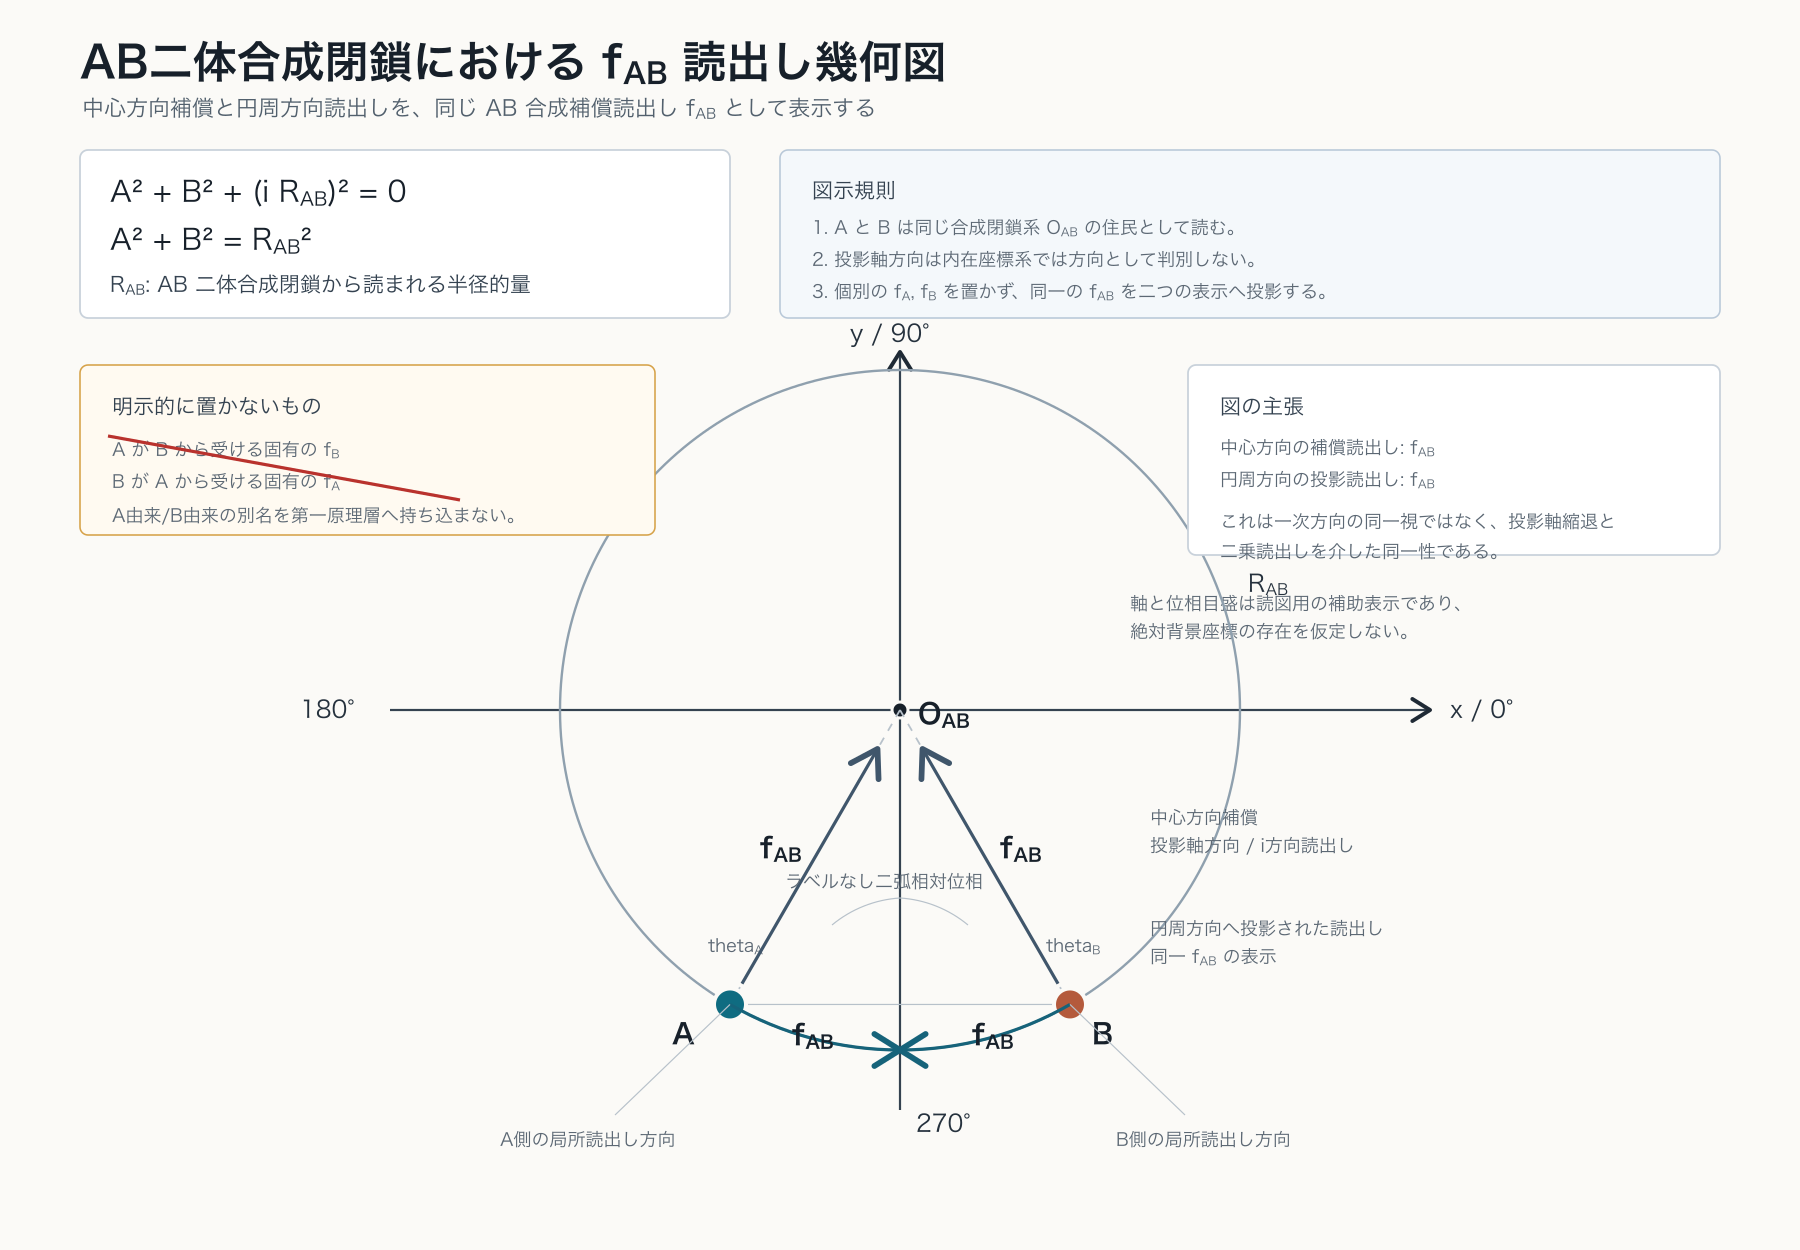
\includegraphics[width=0.45\linewidth,height=\textheight,keepaspectratio,alt={figure}]{AB二体問題の図化_fAB_v1.png}
&
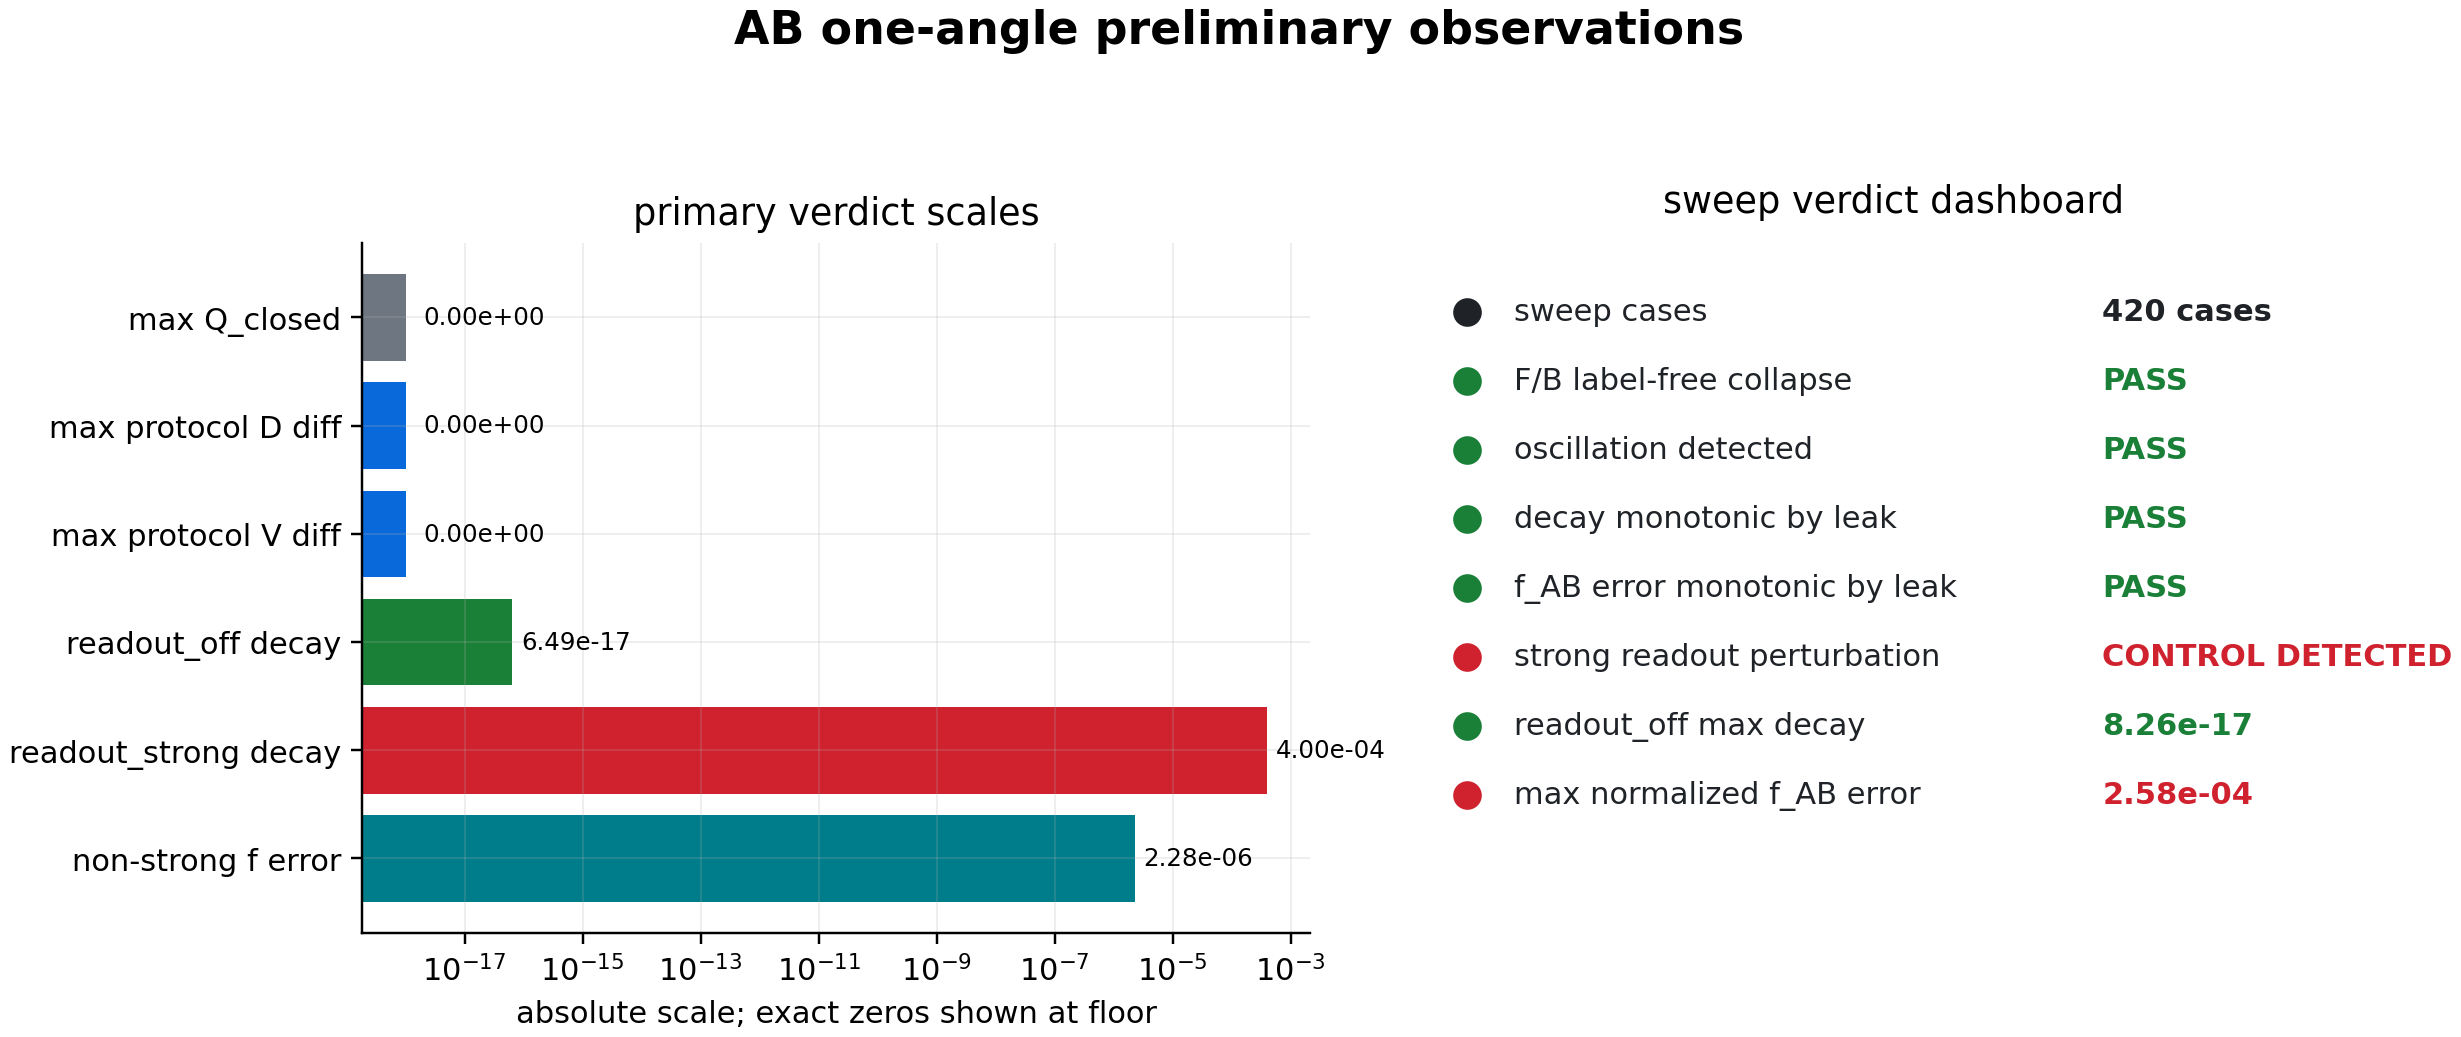
\includegraphics[width=0.45\linewidth,height=\textheight,keepaspectratio,alt={figure}]{ab_two_body_one_angle_harmonic_readout_observation_figures_v1/ab_two_body_one_angle_observation_summary_v1.png} \\
\end{longtable}
}

{\def\LTcaptype{none} % do not increment counter
\begin{longtable}[]{@{}
  >{\raggedright\arraybackslash}p{(\linewidth - 2\tabcolsep) * \real{0.5000}}
  >{\raggedright\arraybackslash}p{(\linewidth - 2\tabcolsep) * \real{0.5000}}@{}}
\toprule\noalign{}
\begin{minipage}[b]{\linewidth}\raggedright
調和状態
\end{minipage} & \begin{minipage}[b]{\linewidth}\raggedright
読出しリーク応答
\end{minipage} \\
\midrule\noalign{}
\endhead
\bottomrule\noalign{}
\endlastfoot
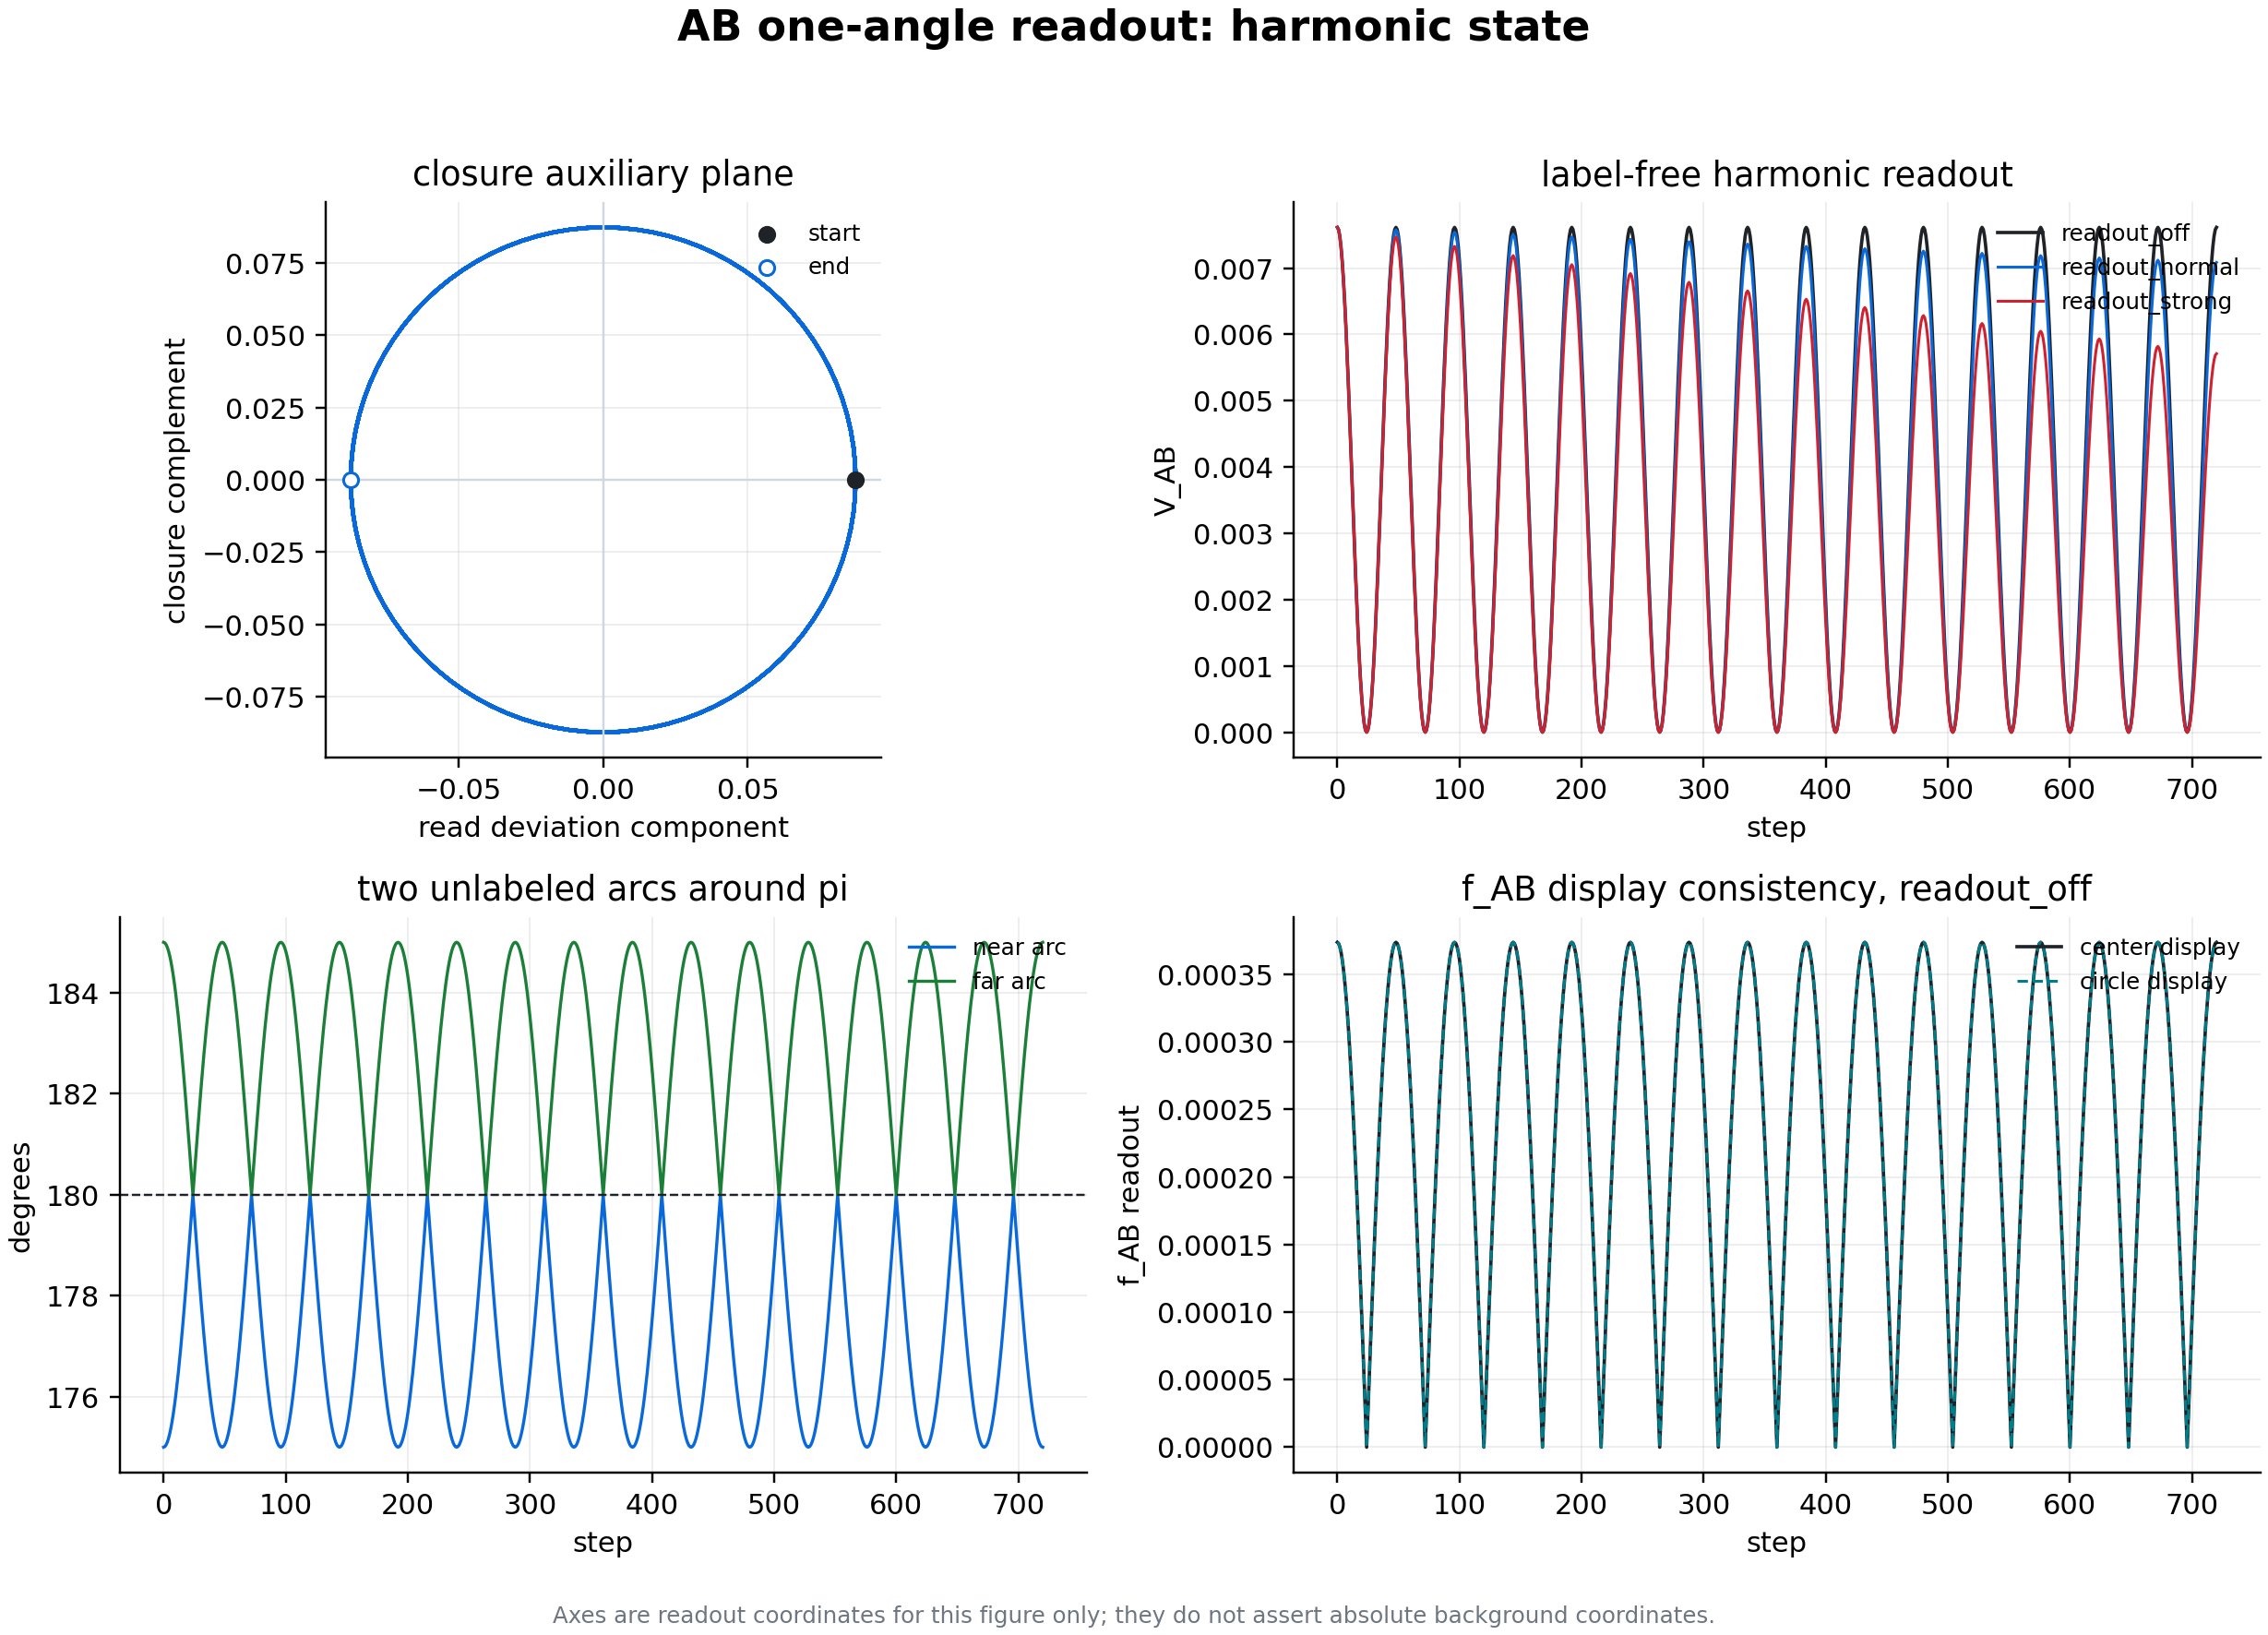
\includegraphics[width=0.45\linewidth,height=\textheight,keepaspectratio,alt={figure}]{ab_two_body_one_angle_harmonic_readout_observation_figures_v1/ab_two_body_one_angle_harmonic_state_v1.png}
&
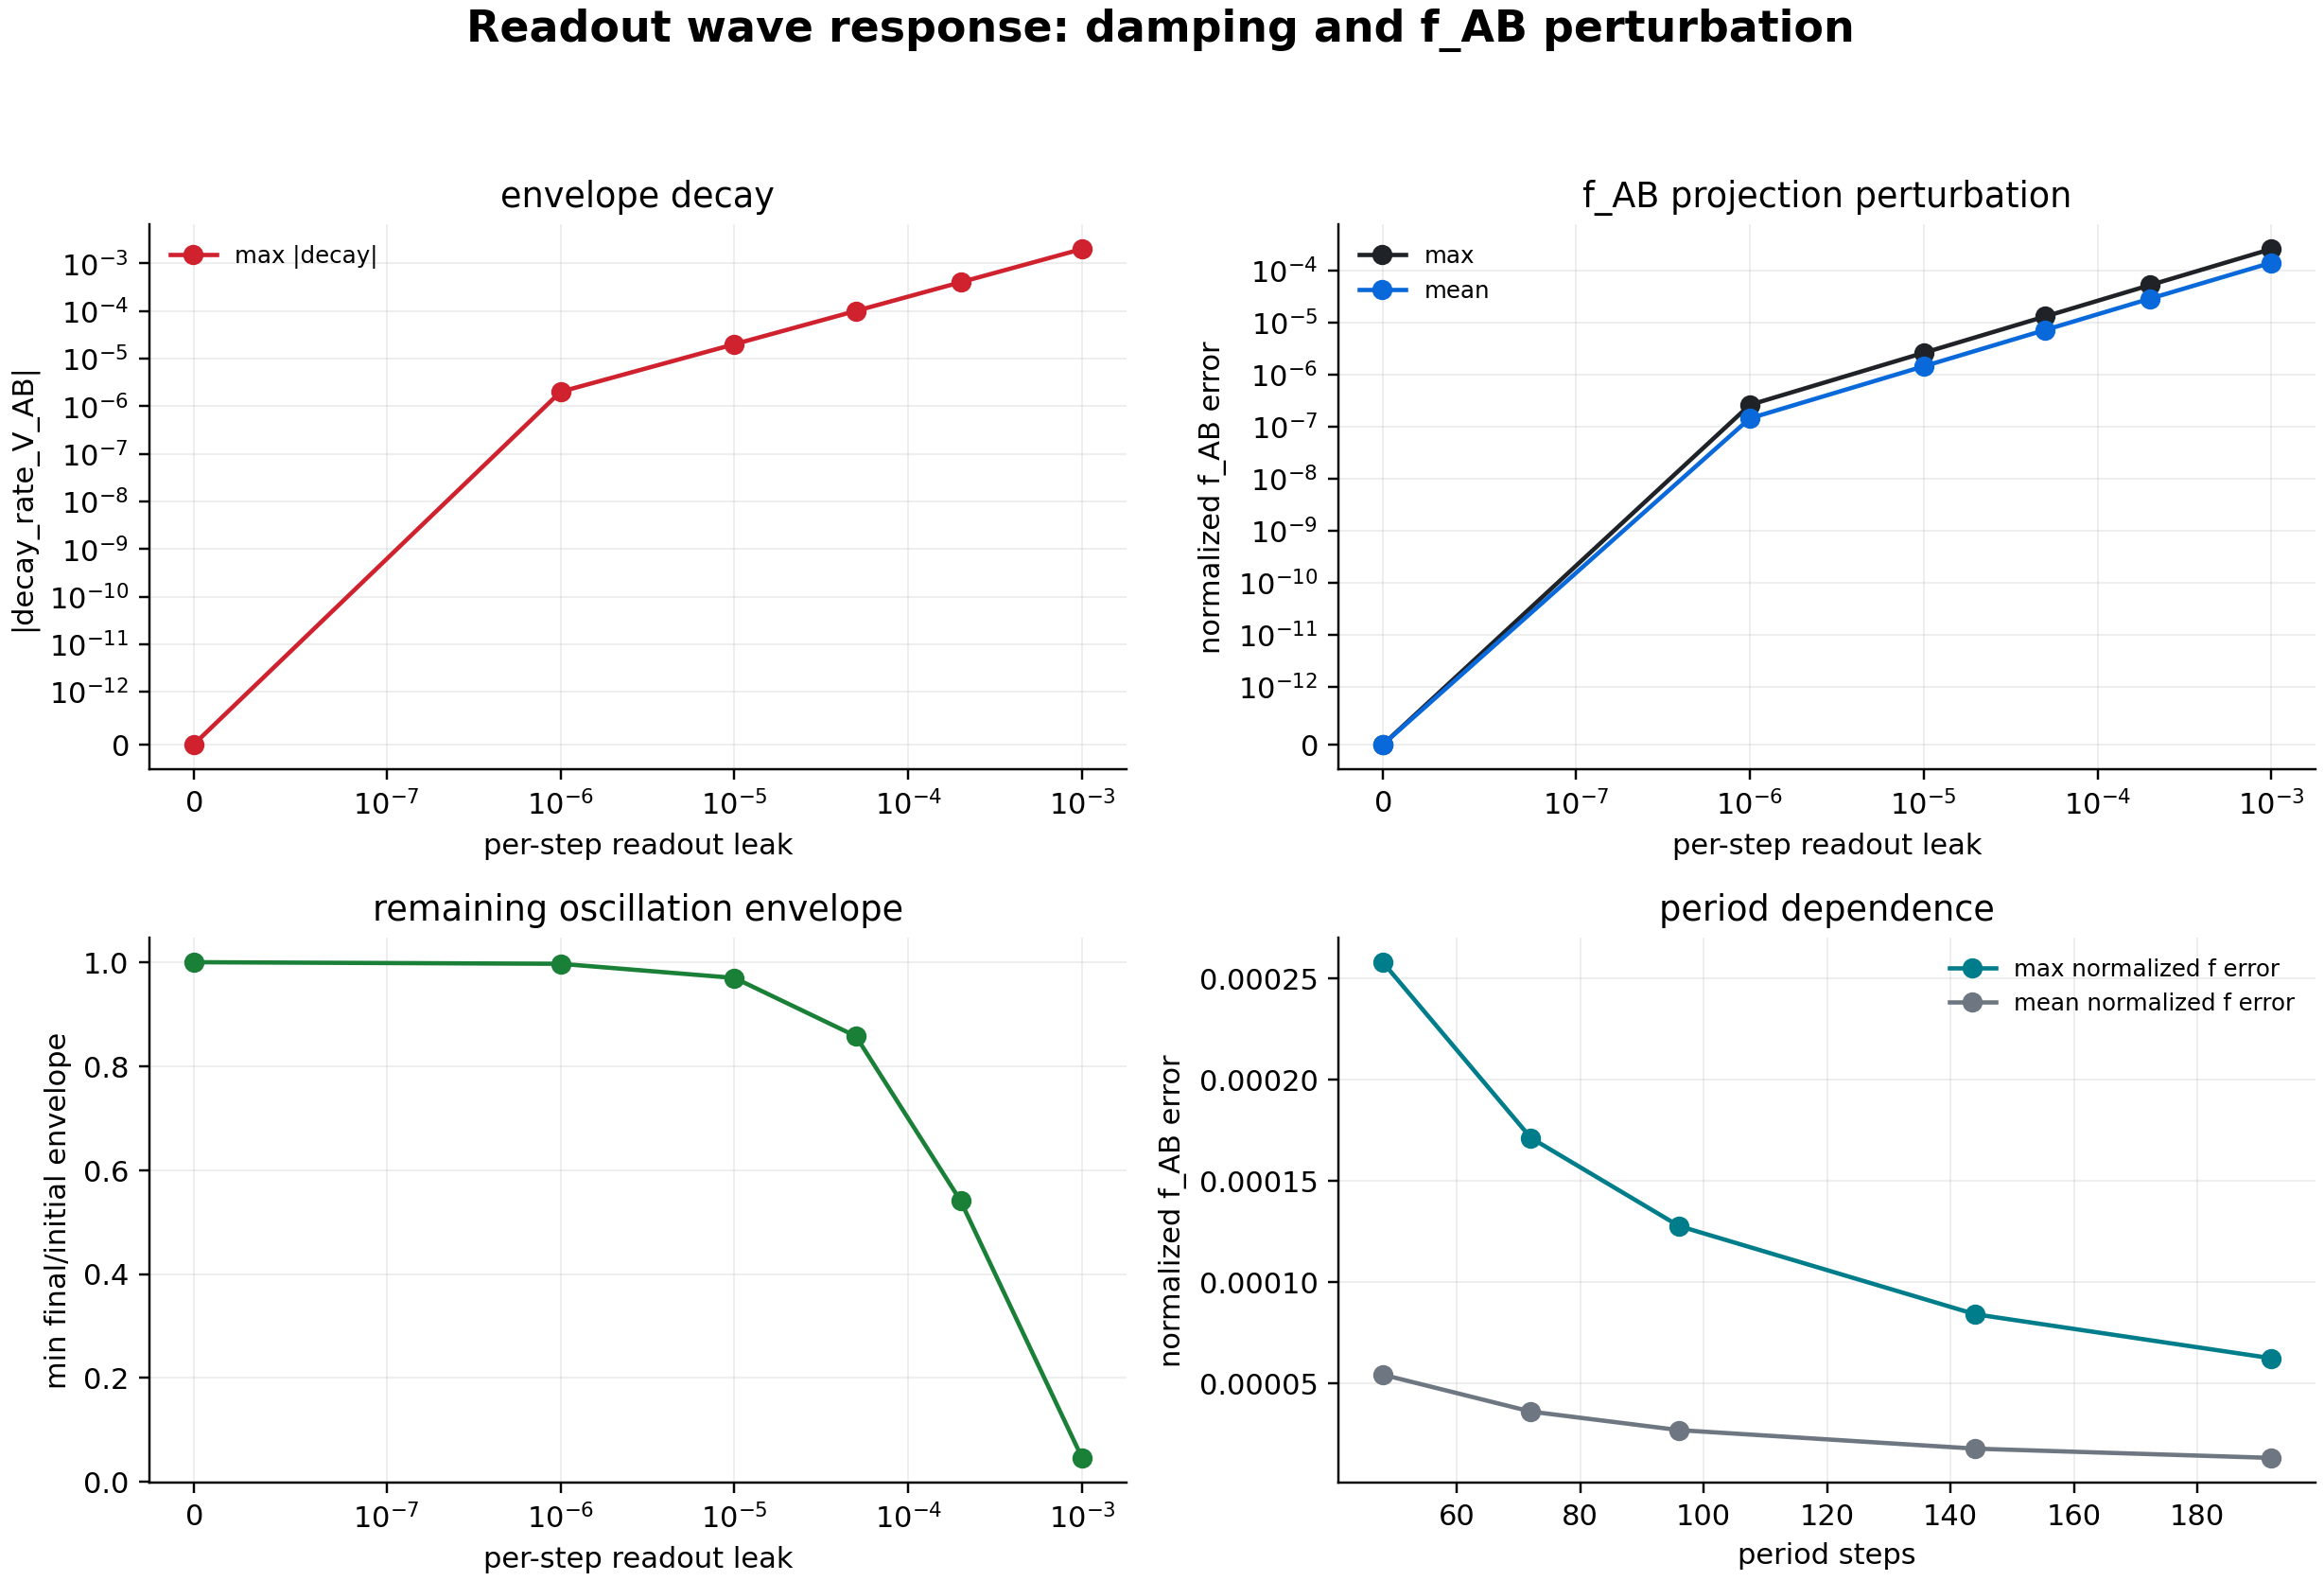
\includegraphics[width=0.45\linewidth,height=\textheight,keepaspectratio,alt={figure}]{ab_two_body_one_angle_harmonic_readout_observation_figures_v1/ab_two_body_one_angle_readout_leak_response_v1.png} \\
\end{longtable}
}

{\def\LTcaptype{none} % do not increment counter
\begin{longtable}[]{@{}
  >{\raggedright\arraybackslash}p{(\linewidth - 2\tabcolsep) * \real{0.5000}}
  >{\raggedright\arraybackslash}p{(\linewidth - 2\tabcolsep) * \real{0.5000}}@{}}
\toprule\noalign{}
\begin{minipage}[b]{\linewidth}\raggedright
Protocol 縮退
\end{minipage} & \begin{minipage}[b]{\linewidth}\raggedright
位相差スケーリング
\end{minipage} \\
\midrule\noalign{}
\endhead
\bottomrule\noalign{}
\endlastfoot
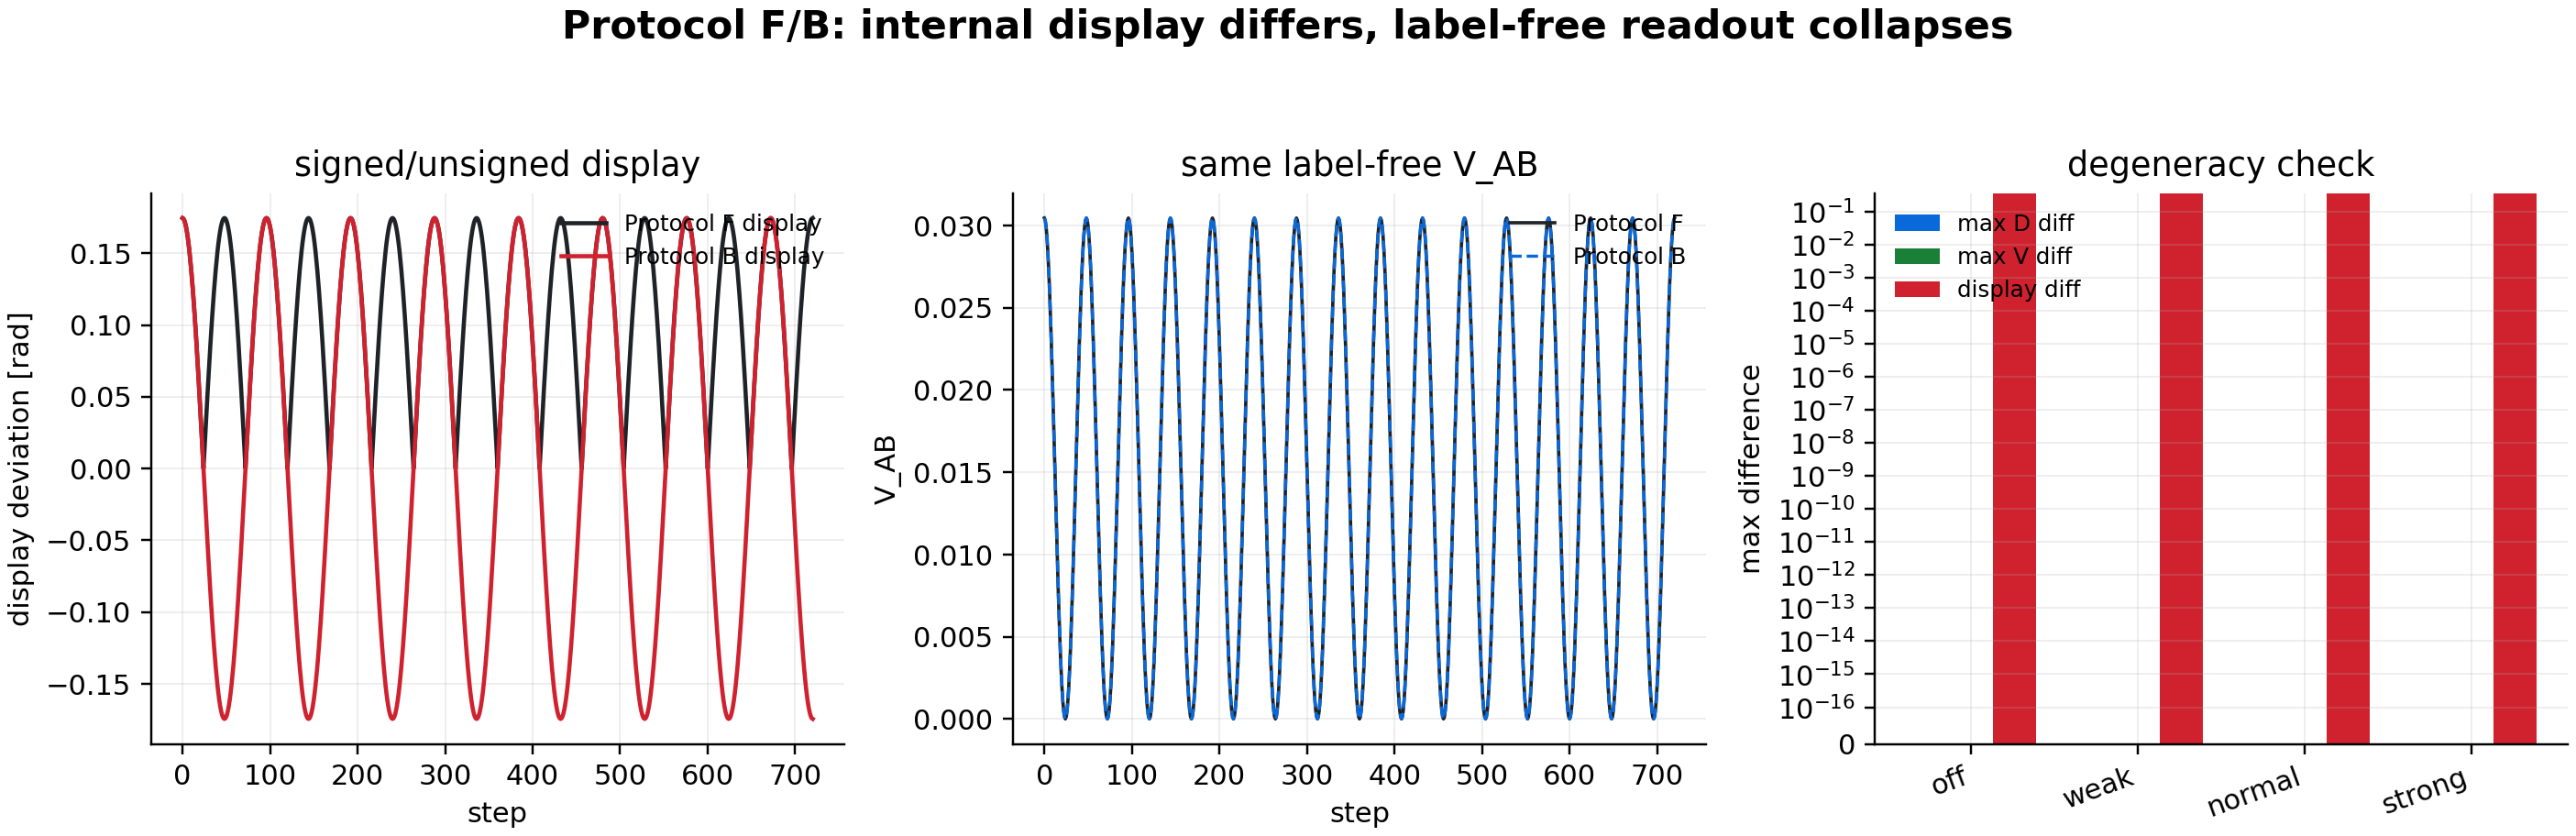
\includegraphics[width=0.45\linewidth,height=\textheight,keepaspectratio,alt={figure}]{ab_two_body_one_angle_harmonic_readout_observation_figures_v1/ab_two_body_one_angle_protocol_degeneracy_v1.png}
&
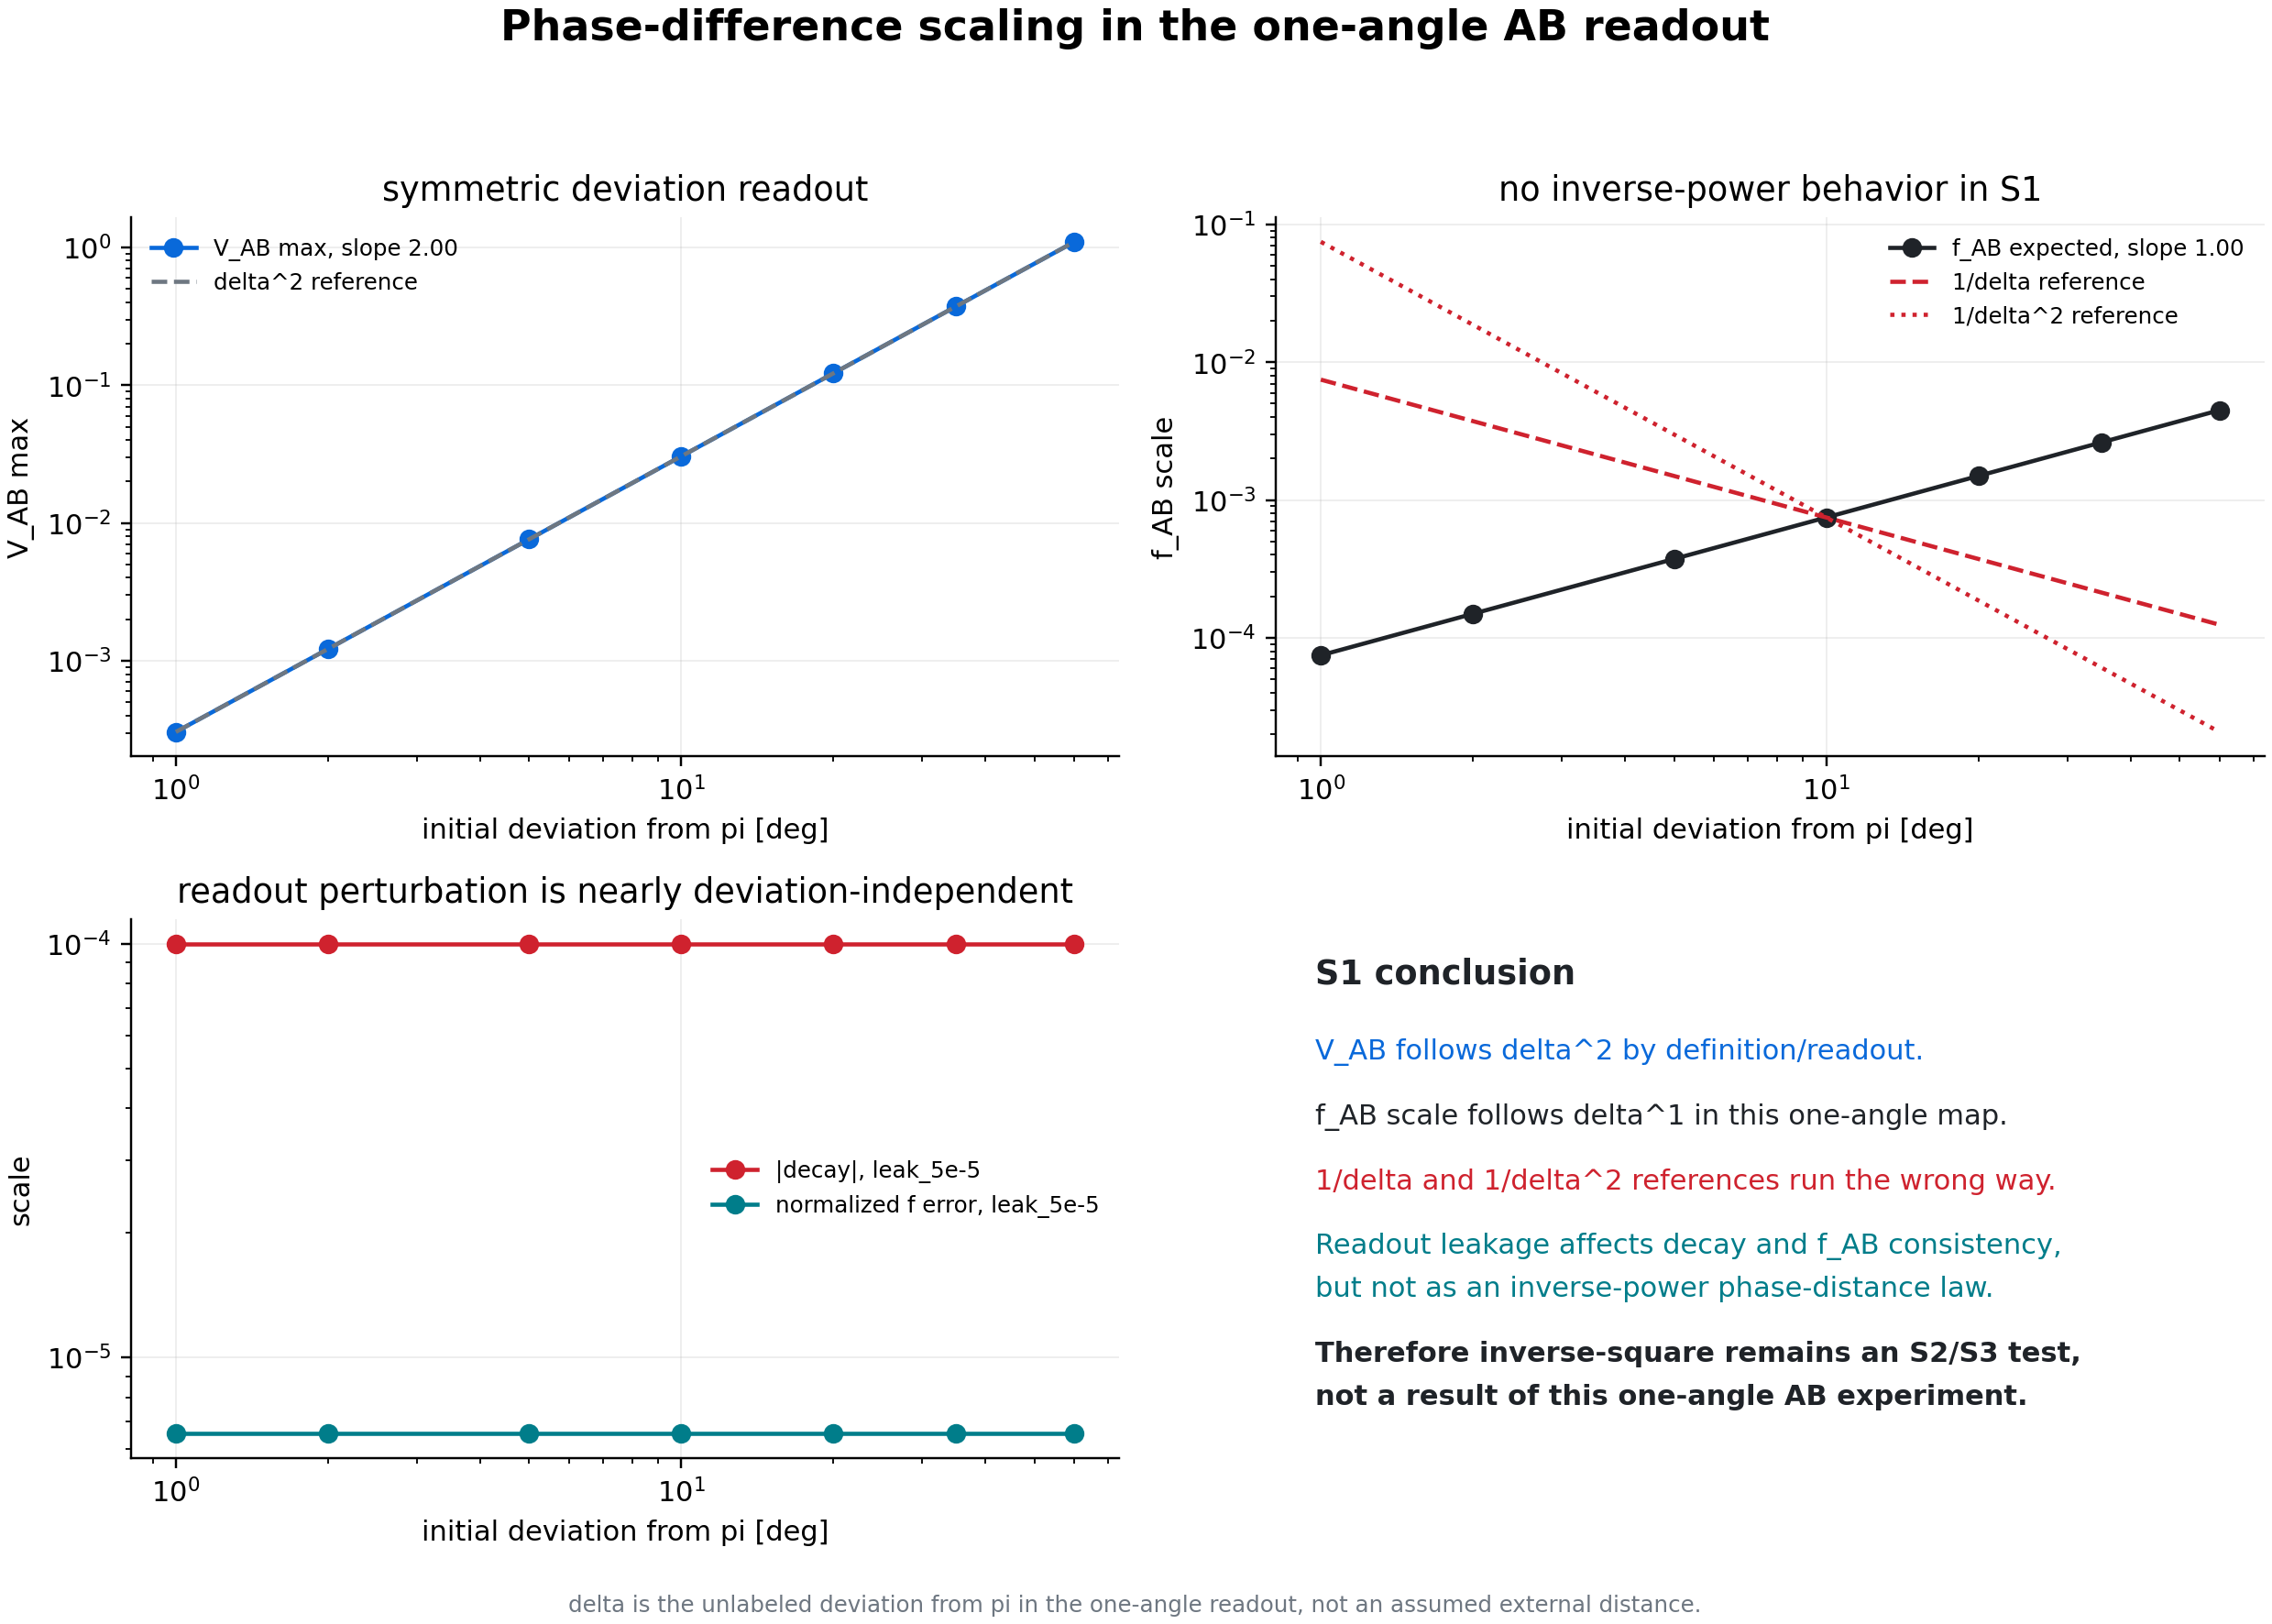
\includegraphics[width=0.45\linewidth,height=\textheight,keepaspectratio,alt={figure}]{ab_two_body_one_angle_harmonic_readout_observation_figures_v1/ab_two_body_one_angle_phase_difference_scaling_v1.png} \\
\end{longtable}
}

\begin{center}\rule{0.5\linewidth}{0.5pt}\end{center}

\subsection{3.
一角度パラメータスイープ}\label{ux4e00ux89d2ux5ea6ux30d1ux30e9ux30e1ux30fcux30bfux30b9ux30a4ux30fcux30d7}

\subsubsection{3.1 主結果}\label{ux4e3bux7d50ux679c-1}

{\def\LTcaptype{none} % do not increment counter
\begin{longtable}[]{@{}lr@{}}
\toprule\noalign{}
量 & 値 \\
\midrule\noalign{}
\endhead
\bottomrule\noalign{}
\endlastfoot
\texttt{sweep\_configuration\_count} & \texttt{210} \\
\texttt{case\_summary\_count} & \texttt{420} \\
\texttt{period\_count} & \texttt{5} \\
\texttt{deviation\_count} & \texttt{7} \\
\texttt{leak\_count} & \texttt{6} \\
\texttt{max\_Q\_closed\_abs} & \texttt{0.0} \\
\texttt{label\_free\_protocol\_degenerate\_all\_cases} &
\texttt{True} \\
\texttt{oscillation\_detected\_all\_cases} & \texttt{True} \\
\texttt{readout\_off\_decay\_max\_abs} & \texttt{8.26e-17} \\
\texttt{decay\_abs\_monotonic\_by\_leak\_all\_grids} & \texttt{True} \\
\texttt{max\_normalized\_f\_AB\_projection\_error} & \texttt{2.58e-4} \\
\end{longtable}
}

本スイープにより、一角度版は弱読出しでは安定である一方、強い読出し波は
\texttt{f\_AB} 射影を歪めることが確認された。

{\def\LTcaptype{none} % do not increment counter
\begin{longtable}[]{@{}
  >{\raggedright\arraybackslash}p{(\linewidth - 2\tabcolsep) * \real{0.5000}}
  >{\raggedright\arraybackslash}p{(\linewidth - 2\tabcolsep) * \real{0.5000}}@{}}
\toprule\noalign{}
\begin{minipage}[b]{\linewidth}\raggedright
漏れ量と射影誤差
\end{minipage} & \begin{minipage}[b]{\linewidth}\raggedright
漏れ量と減衰
\end{minipage} \\
\midrule\noalign{}
\endhead
\bottomrule\noalign{}
\endlastfoot
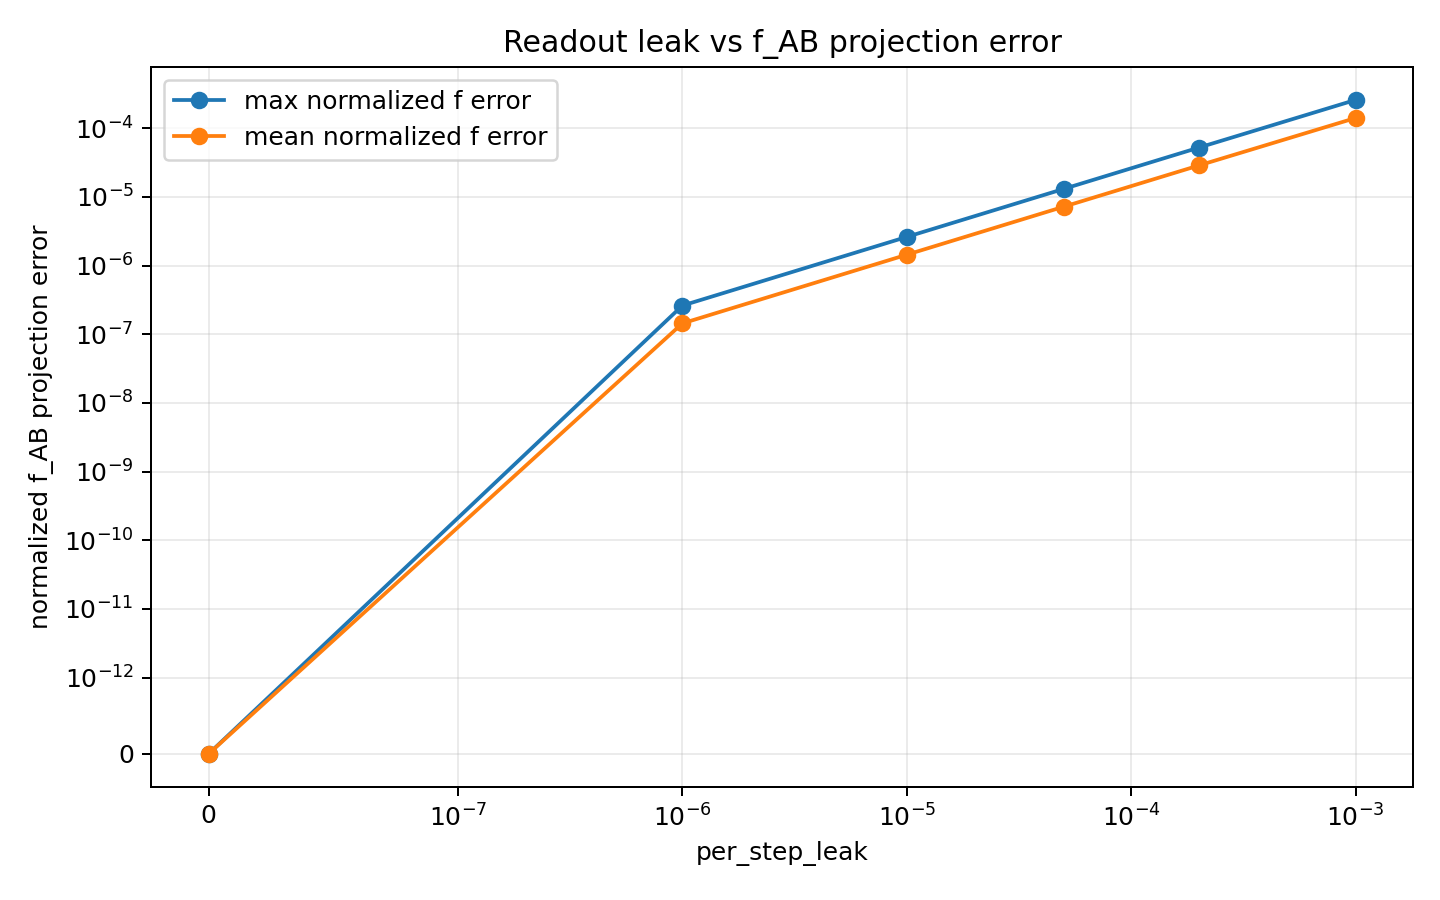
\includegraphics[width=0.45\linewidth,height=\textheight,keepaspectratio,alt={figure}]{ab_two_body_one_angle_harmonic_readout_parameter_sweep_preliminary_result_v1/ab_two_body_one_angle_parameter_sweep_leak_f_error_v1.png}
&
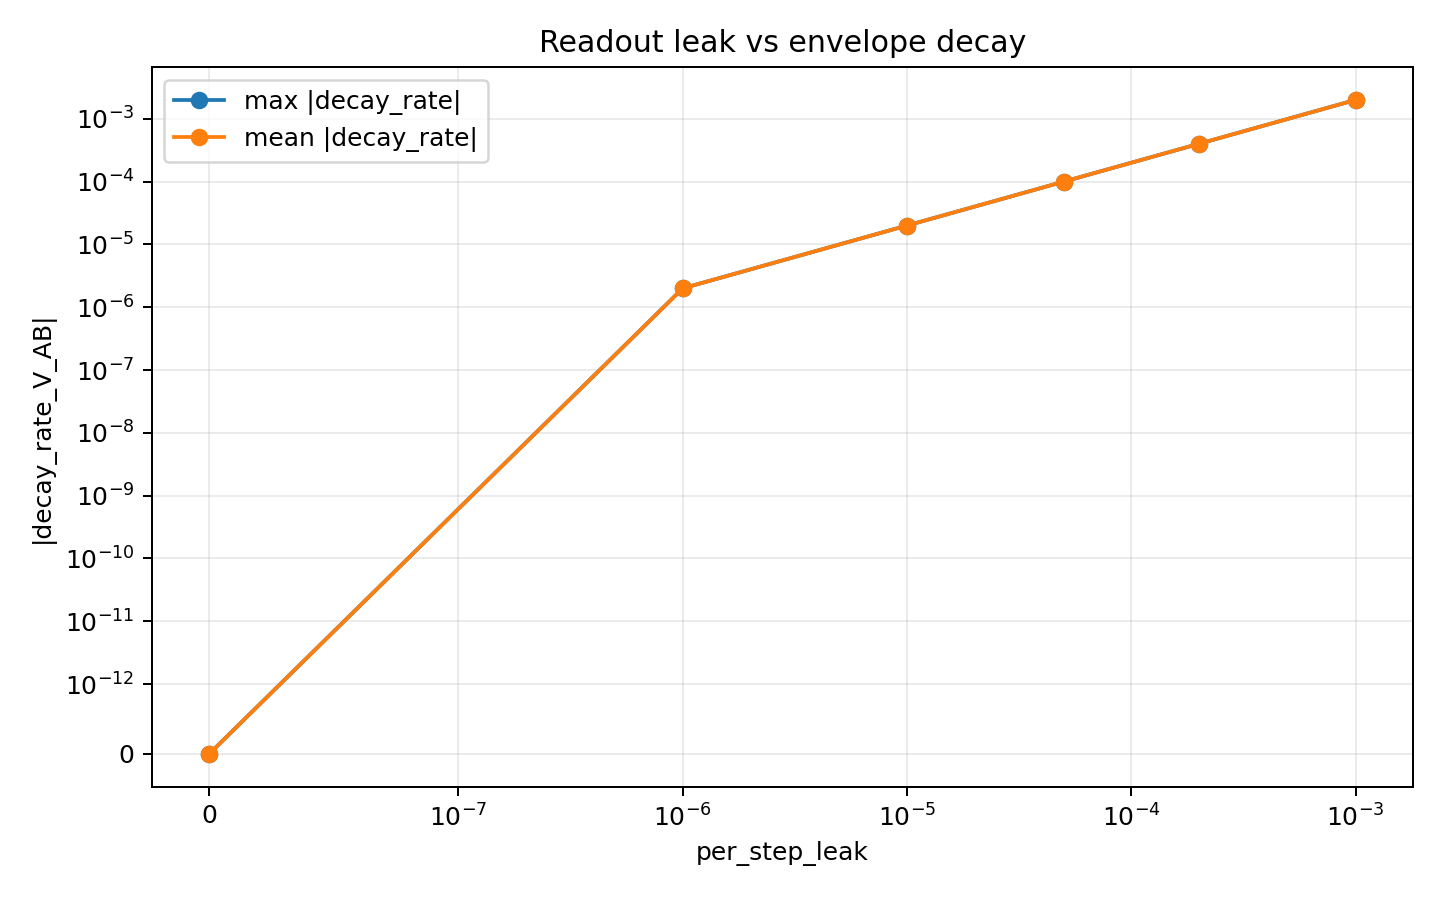
\includegraphics[width=0.45\linewidth,height=\textheight,keepaspectratio,alt={figure}]{ab_two_body_one_angle_harmonic_readout_parameter_sweep_preliminary_result_v1/ab_two_body_one_angle_parameter_sweep_leak_decay_v1.png} \\
\end{longtable}
}

{\def\LTcaptype{none} % do not increment counter
\begin{longtable}[]{@{}
  >{\raggedright\arraybackslash}p{(\linewidth - 2\tabcolsep) * \real{0.5000}}
  >{\raggedright\arraybackslash}p{(\linewidth - 2\tabcolsep) * \real{0.5000}}@{}}
\toprule\noalign{}
\begin{minipage}[b]{\linewidth}\raggedright
周期スイープ
\end{minipage} & \begin{minipage}[b]{\linewidth}\raggedright
選択時系列
\end{minipage} \\
\midrule\noalign{}
\endhead
\bottomrule\noalign{}
\endlastfoot
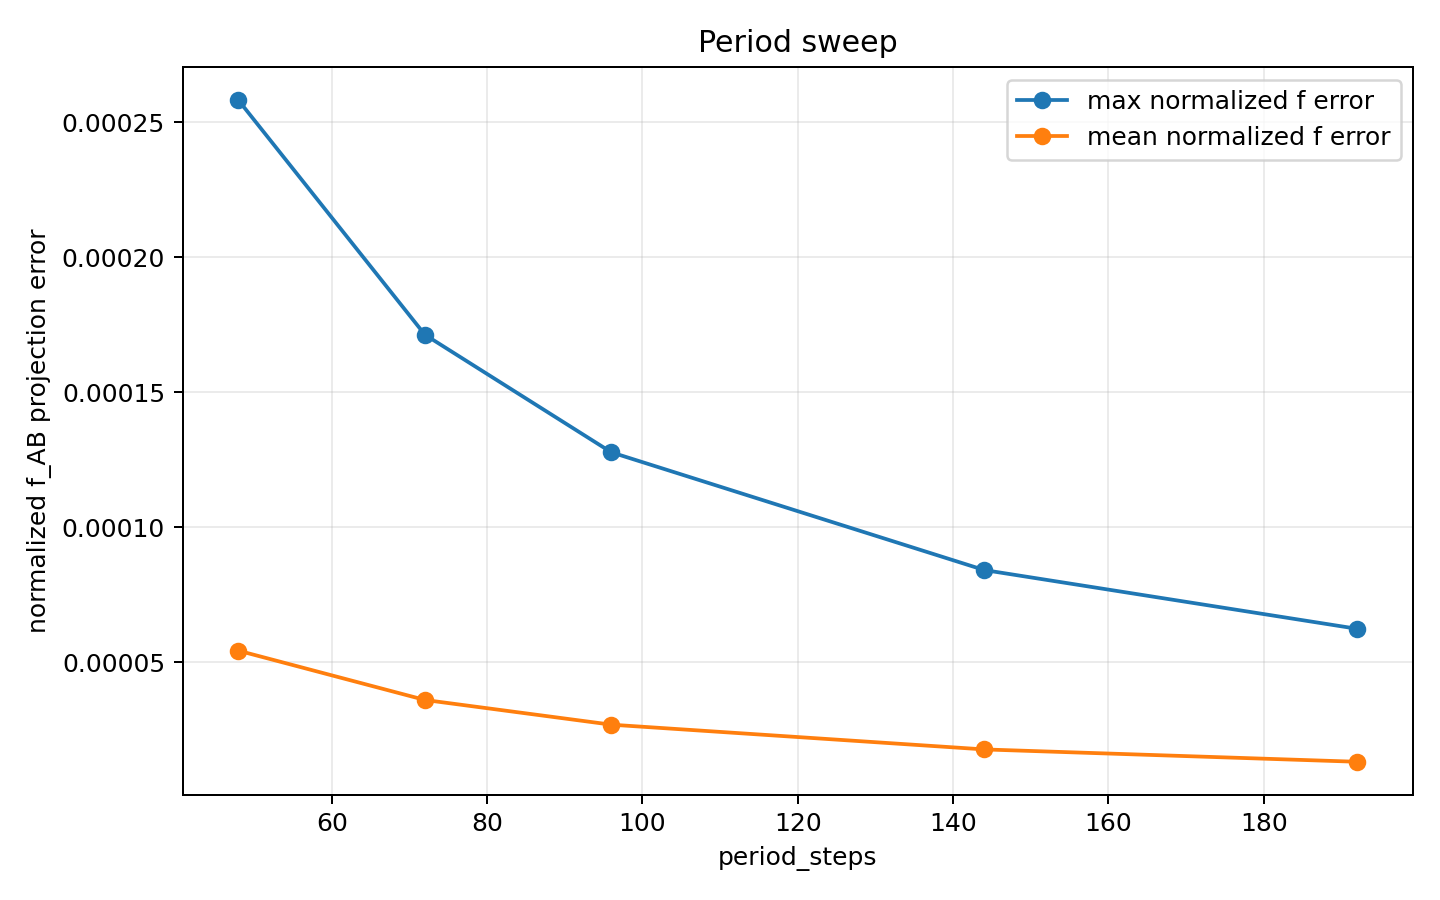
\includegraphics[width=0.45\linewidth,height=\textheight,keepaspectratio,alt={figure}]{ab_two_body_one_angle_harmonic_readout_parameter_sweep_preliminary_result_v1/ab_two_body_one_angle_parameter_sweep_period_v1.png}
&
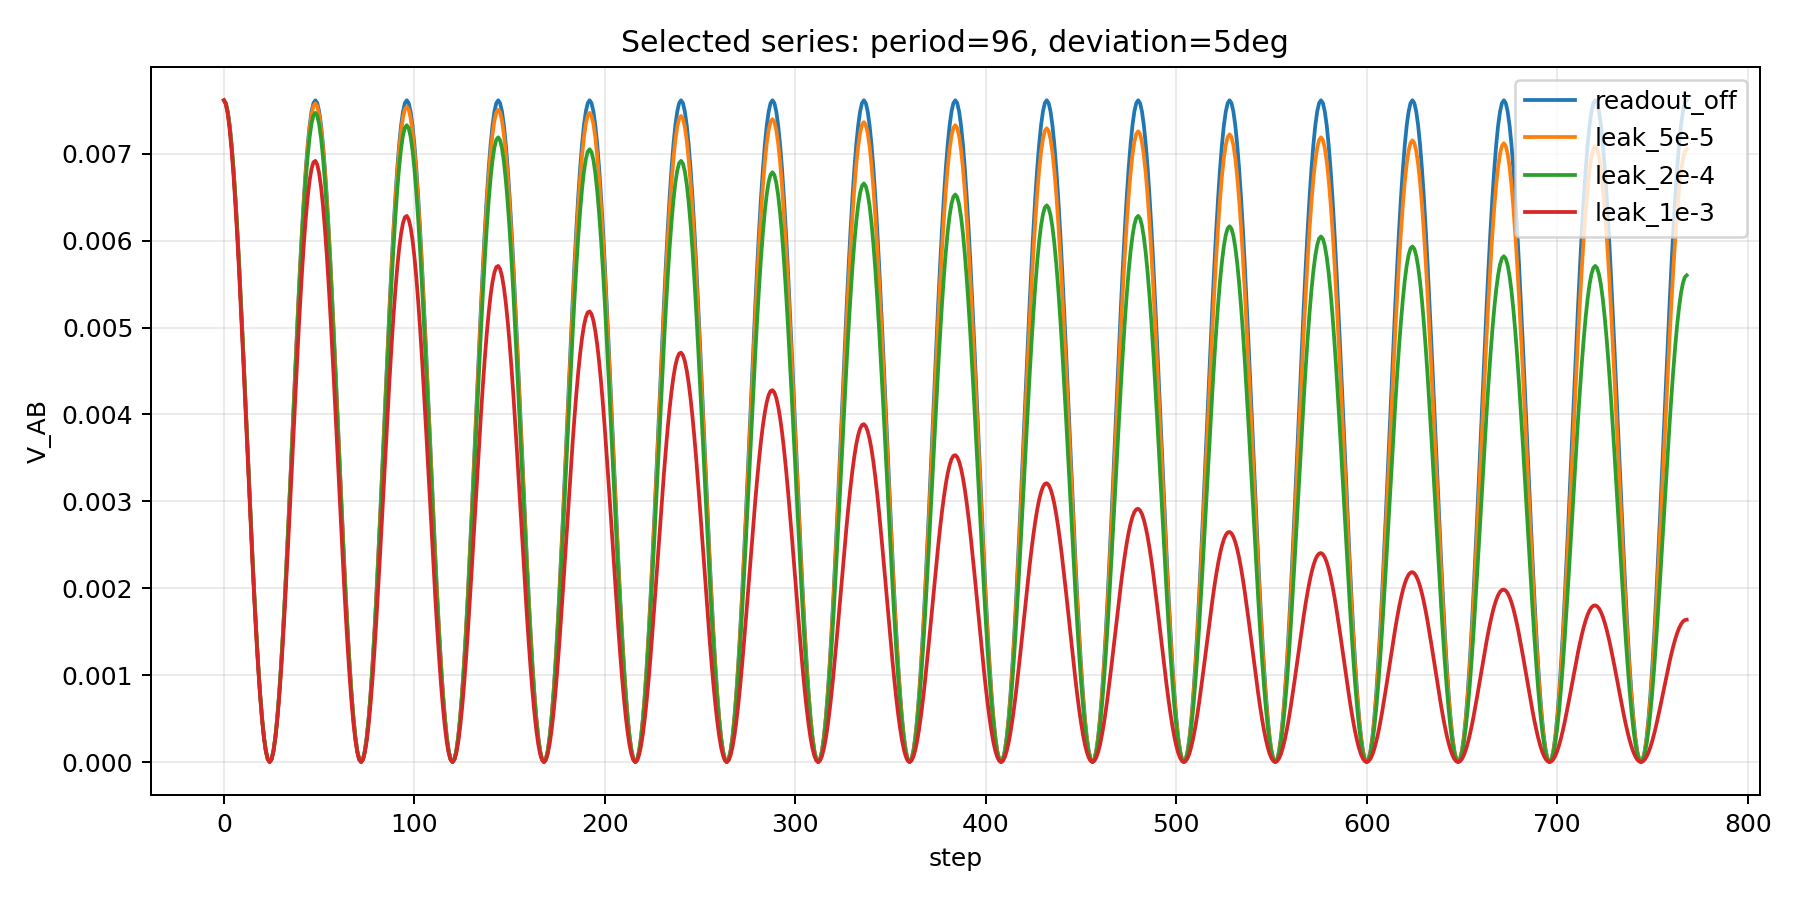
\includegraphics[width=0.45\linewidth,height=\textheight,keepaspectratio,alt={figure}]{ab_two_body_one_angle_harmonic_readout_parameter_sweep_preliminary_result_v1/ab_two_body_one_angle_parameter_sweep_selected_series_v1.png} \\
\end{longtable}
}

\begin{center}\rule{0.5\linewidth}{0.5pt}\end{center}

\subsection{4.
c=1内部較正とchi-tau面積スイープ}\label{c1ux5185ux90e8ux8f03ux6b63ux3068chi-tauux9762ux7a4dux30b9ux30a4ux30fcux30d7}

\subsubsection{4.1 実験の意味}\label{ux5b9fux9a13ux306eux610fux5473-1}

一角度調和読出しでは、位相差に応じた距離減衰は読めなかった。

そこで、実験ステップ \texttt{s}
を時間そのものとして扱わず、独立な時間位相候補

\begin{Shaded}
\begin{Highlighting}[]
\NormalTok{tau\_read}
\end{Highlighting}
\end{Shaded}

を導入した。

目的は、

\begin{Shaded}
\begin{Highlighting}[]
\NormalTok{chi\_read と tau\_read が独立な面を作るか}
\end{Highlighting}
\end{Shaded}

を検査することである。

\subsubsection{4.2 主結果}\label{ux4e3bux7d50ux679c-2}

{\def\LTcaptype{none} % do not increment counter
\begin{longtable}[]{@{}lr@{}}
\toprule\noalign{}
量 & 値 \\
\midrule\noalign{}
\endhead
\bottomrule\noalign{}
\endlastfoot
\texttt{case\_summary\_count} & \texttt{288} \\
\texttt{power\_candidate\_count} & \texttt{48} \\
\texttt{max\_Q\_closed\_abs} & \texttt{0.0} \\
\texttt{disabled\_max\_area} & \texttt{0.0} \\
\texttt{locked\_max\_area} & \texttt{7.11e-15} \\
\texttt{independent\_min\_area} & \texttt{0.0024367633602631385} \\
\texttt{c1\_readout\_off\_max\_epsilon\_c\_abs} & \texttt{2.33e-15} \\
\texttt{c1\_area\_sweep\_detected\_all\_cases} & \texttt{True} \\
\texttt{tau\_is\_step\_used\_any} & \texttt{False} \\
\texttt{external\_c\_used\_any} & \texttt{False} \\
\end{longtable}
}

成立したことは次である。

\begin{Shaded}
\begin{Highlighting}[]
\NormalTok{tau disabled は面積を作らない。}
\NormalTok{tau locked は面積を作らない。}
\NormalTok{tau independent は chi{-}tau 面積を作る。}
\end{Highlighting}
\end{Shaded}

したがって、時間位相を独立に読めば \texttt{chi-tau} 面は立つ。

しかし、それだけでは距離減衰は出ない。

\subsubsection{4.3 図}\label{ux56f3-1}

{\def\LTcaptype{none} % do not increment counter
\begin{longtable}[]{@{}
  >{\raggedright\arraybackslash}p{(\linewidth - 2\tabcolsep) * \real{0.5000}}
  >{\raggedright\arraybackslash}p{(\linewidth - 2\tabcolsep) * \real{0.5000}}@{}}
\toprule\noalign{}
\begin{minipage}[b]{\linewidth}\raggedright
\texttt{chi-tau} 面
\end{minipage} & \begin{minipage}[b]{\linewidth}\raggedright
面積スイープ
\end{minipage} \\
\midrule\noalign{}
\endhead
\bottomrule\noalign{}
\endlastfoot
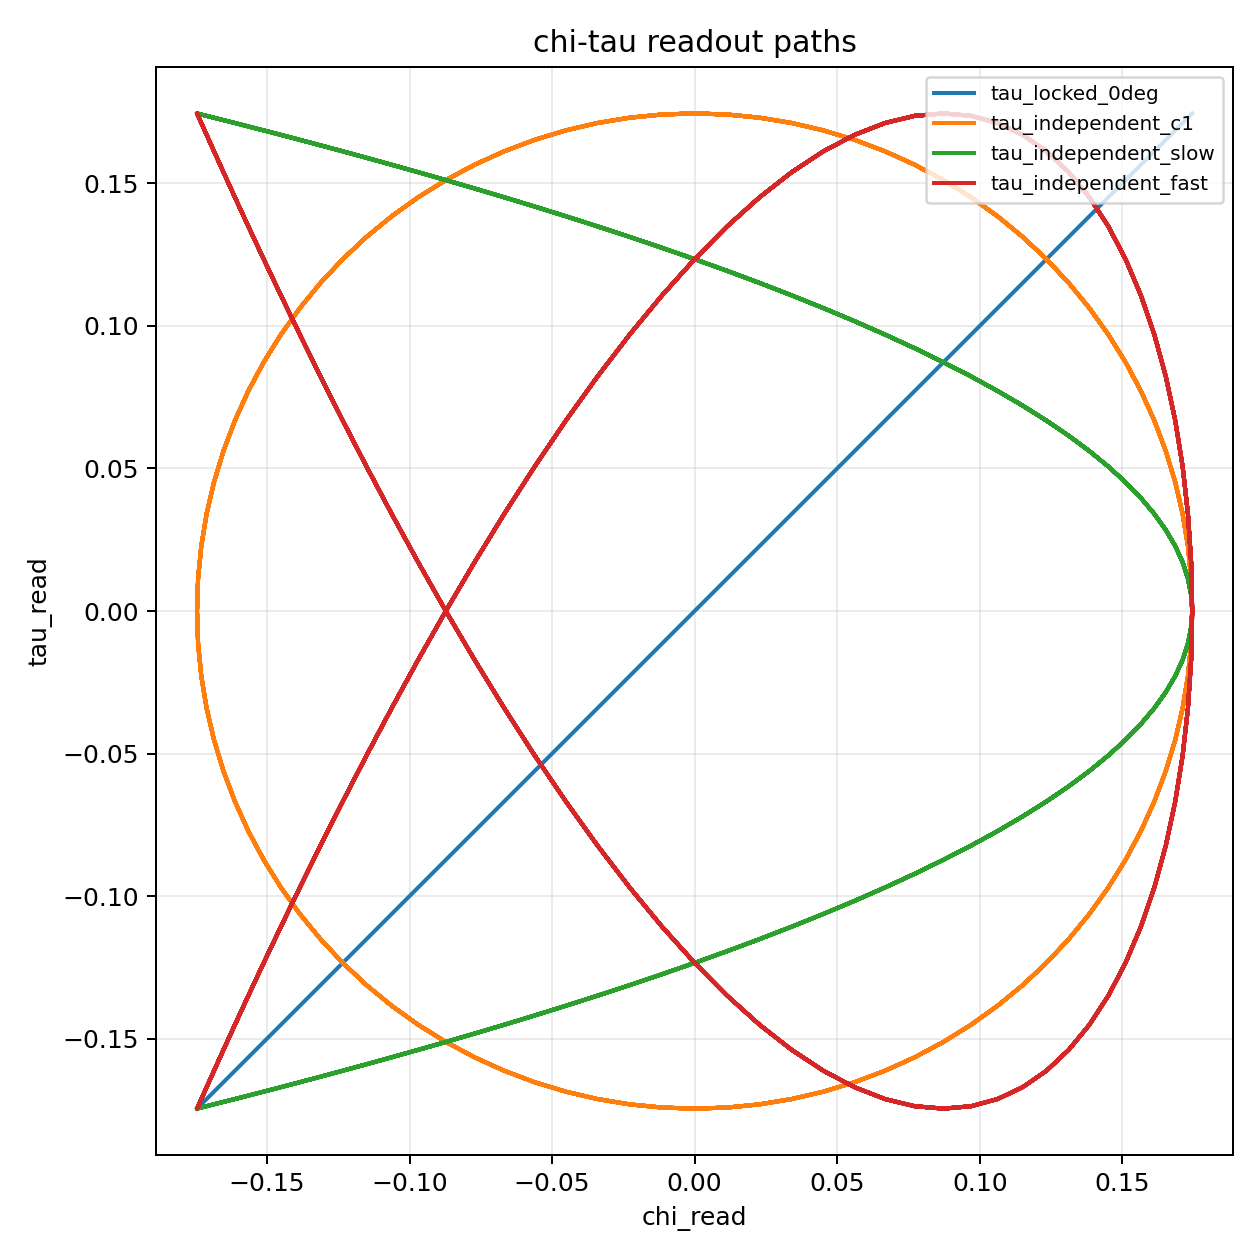
\includegraphics[width=0.45\linewidth,height=\textheight,keepaspectratio,alt={figure}]{ab_two_body_c1_internal_calibration_chi_tau_area_sweep_preliminary_result_v1/ab_two_body_c1_internal_calibration_chi_tau_surface_v1.png}
&
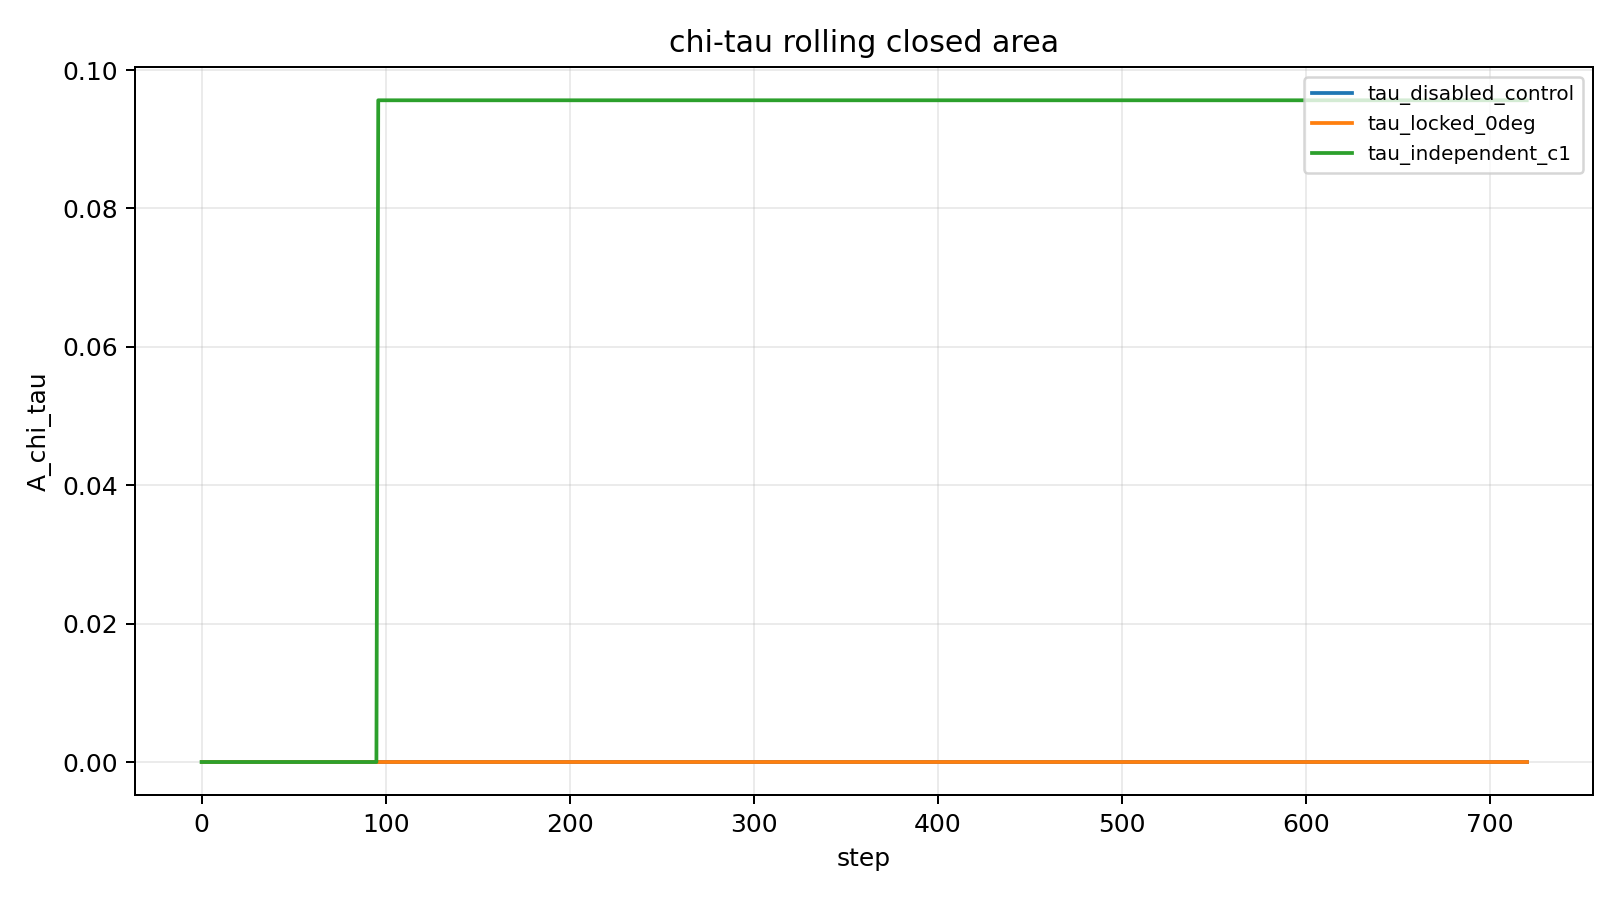
\includegraphics[width=0.45\linewidth,height=\textheight,keepaspectratio,alt={figure}]{ab_two_body_c1_internal_calibration_chi_tau_area_sweep_preliminary_result_v1/ab_two_body_c1_internal_calibration_area_sweep_v1.png} \\
\end{longtable}
}

{\def\LTcaptype{none} % do not increment counter
\begin{longtable}[]{@{}
  >{\raggedright\arraybackslash}p{(\linewidth - 2\tabcolsep) * \real{0.5000}}
  >{\raggedright\arraybackslash}p{(\linewidth - 2\tabcolsep) * \real{0.5000}}@{}}
\toprule\noalign{}
\begin{minipage}[b]{\linewidth}\raggedright
\texttt{c=1} 較正誤差
\end{minipage} & \begin{minipage}[b]{\linewidth}\raggedright
冪候補
\end{minipage} \\
\midrule\noalign{}
\endhead
\bottomrule\noalign{}
\endlastfoot
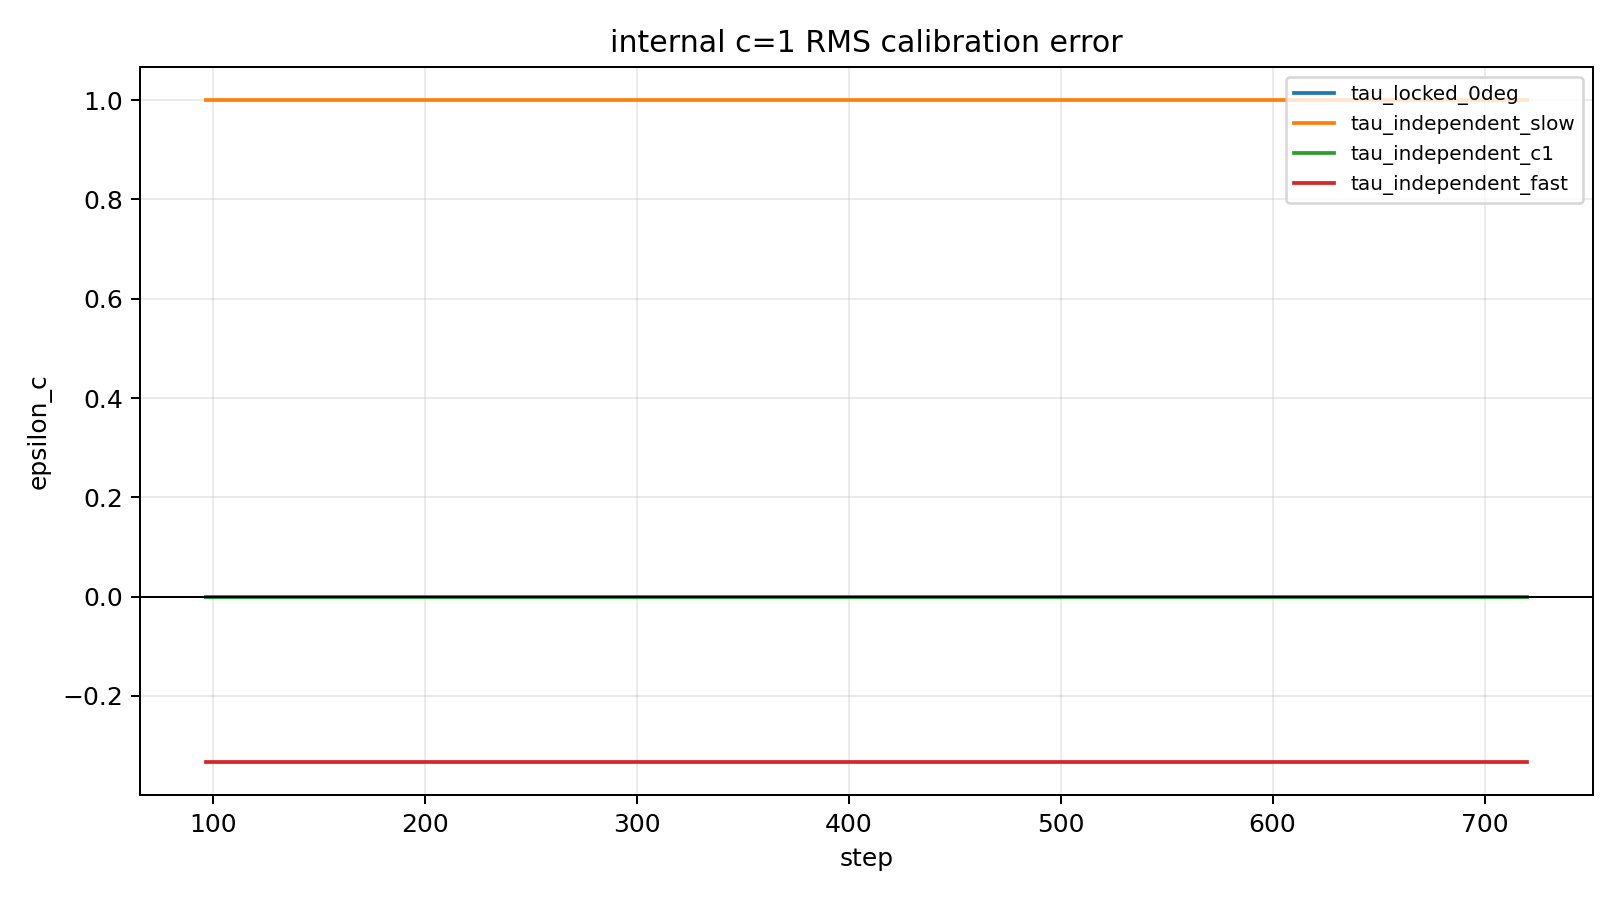
\includegraphics[width=0.45\linewidth,height=\textheight,keepaspectratio,alt={figure}]{ab_two_body_c1_internal_calibration_chi_tau_area_sweep_preliminary_result_v1/ab_two_body_c1_internal_calibration_error_v1.png}
&
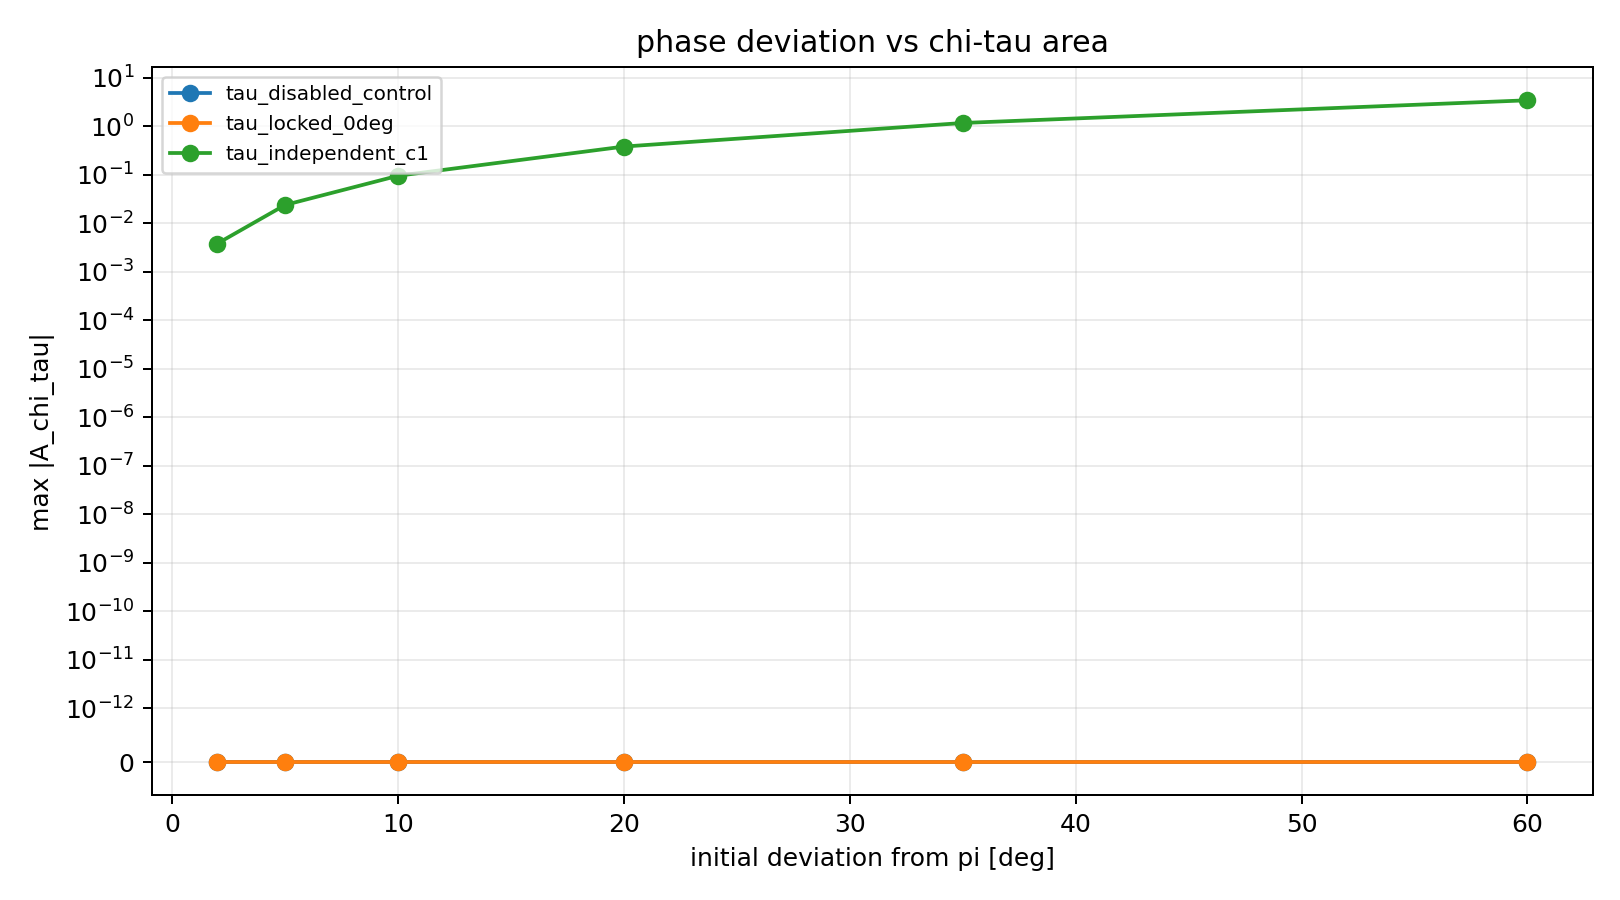
\includegraphics[width=0.45\linewidth,height=\textheight,keepaspectratio,alt={figure}]{ab_two_body_c1_internal_calibration_chi_tau_area_sweep_preliminary_result_v1/ab_two_body_c1_internal_calibration_power_candidate_v1.png} \\
\end{longtable}
}

{\def\LTcaptype{none} % do not increment counter
\begin{longtable}[]{@{}
  >{\raggedright\arraybackslash}p{(\linewidth - 0\tabcolsep) * \real{1.0000}}@{}}
\toprule\noalign{}
\begin{minipage}[b]{\linewidth}\raggedright
読出しリーク
\end{minipage} \\
\midrule\noalign{}
\endhead
\bottomrule\noalign{}
\endlastfoot
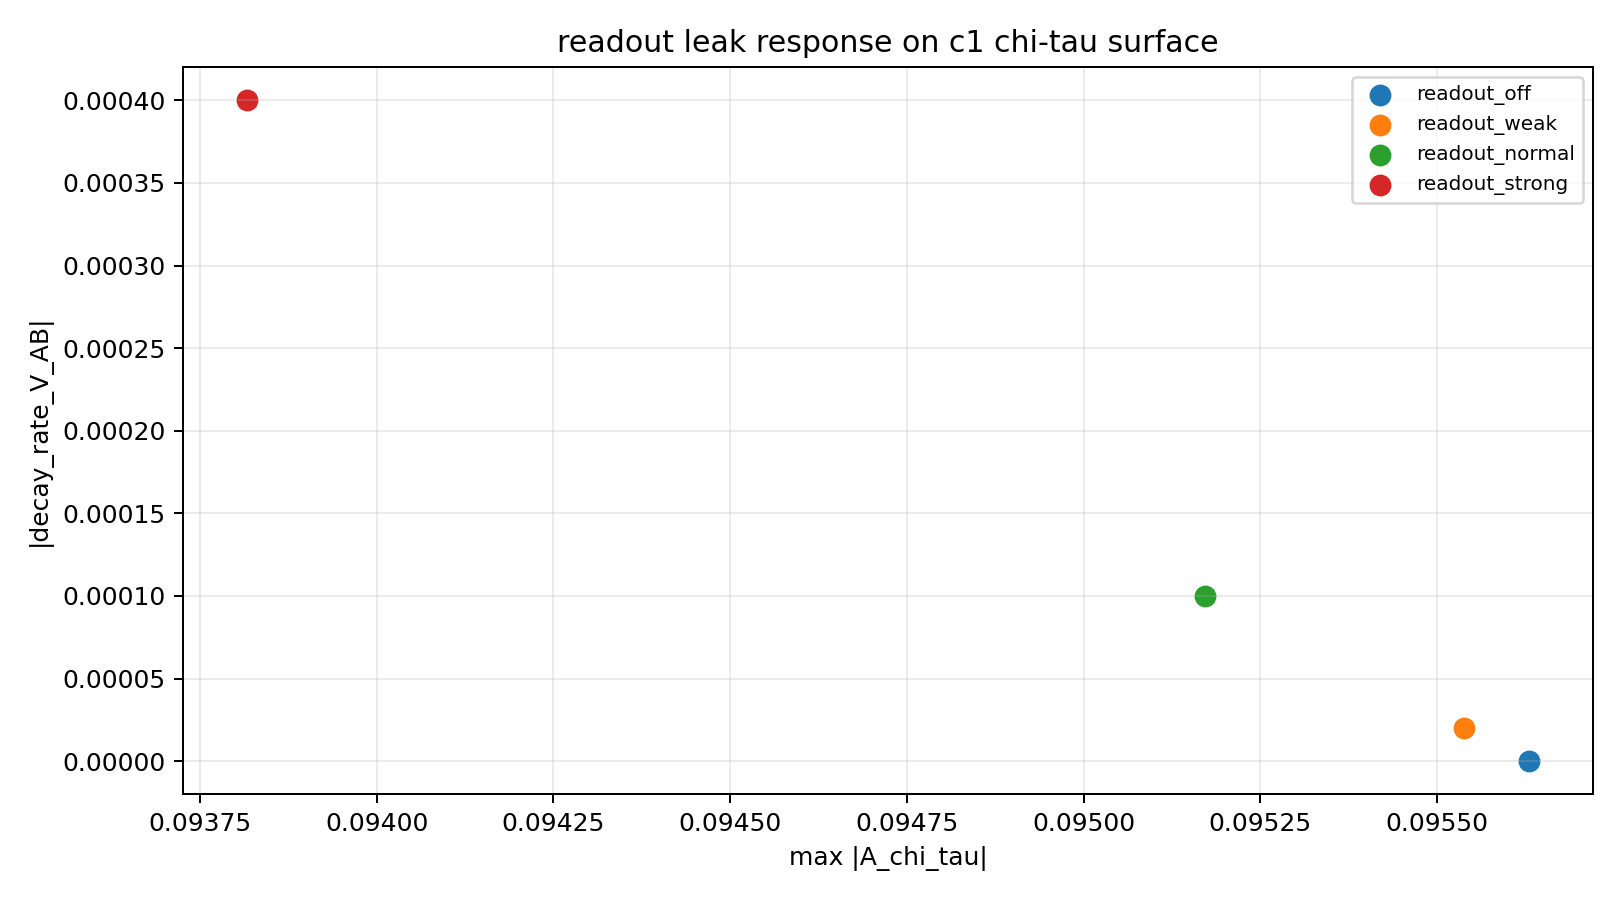
\includegraphics[width=0.65\linewidth,height=\textheight,keepaspectratio,alt={figure}]{ab_two_body_c1_internal_calibration_chi_tau_area_sweep_preliminary_result_v1/ab_two_body_c1_internal_calibration_readout_leak_v1.png} \\
\end{longtable}
}

\begin{center}\rule{0.5\linewidth}{0.5pt}\end{center}

\subsection{5.
c=1内部較正パラメータスイープ}\label{c1ux5185ux90e8ux8f03ux6b63ux30d1ux30e9ux30e1ux30fcux30bfux30b9ux30a4ux30fcux30d7}

\subsubsection{5.1 主結果}\label{ux4e3bux7d50ux679c-3}

{\def\LTcaptype{none} % do not increment counter
\begin{longtable}[]{@{}lr@{}}
\toprule\noalign{}
量 & 値 \\
\midrule\noalign{}
\endhead
\bottomrule\noalign{}
\endlastfoot
\texttt{sweep\_case\_count} & \texttt{756} \\
\texttt{readout\_off\_case\_count} & \texttt{252} \\
\texttt{rank2\_readout\_off\_count} & \texttt{246} \\
\texttt{c1\_surface\_like\_readout\_off\_count} & \texttt{13} \\
\texttt{c1\_locked\_like\_readout\_off\_count} & \texttt{8} \\
\texttt{min\_c\_error\_readout\_off} & \texttt{1.11e-15} \\
\texttt{max\_area\_readout\_off} & \texttt{0.19685536479742288} \\
\end{longtable}
}

この結果により、

\begin{Shaded}
\begin{Highlighting}[]
\NormalTok{c=1}
\NormalTok{rank\_chi\_tau = 2}
\NormalTok{A\_chi\_tau != 0}
\end{Highlighting}
\end{Shaded}

の三条件を同時に要求する必要が明確になった。

\texttt{c=1} に近いだけでは、\texttt{chi-tau} 面が成立したとは言えない。

{\def\LTcaptype{none} % do not increment counter
\begin{longtable}[]{@{}
  >{\raggedright\arraybackslash}p{(\linewidth - 2\tabcolsep) * \real{0.5000}}
  >{\raggedright\arraybackslash}p{(\linewidth - 2\tabcolsep) * \real{0.5000}}@{}}
\toprule\noalign{}
\begin{minipage}[b]{\linewidth}\raggedright
c 誤差 heatmap
\end{minipage} & \begin{minipage}[b]{\linewidth}\raggedright
面積 heatmap
\end{minipage} \\
\midrule\noalign{}
\endhead
\bottomrule\noalign{}
\endlastfoot
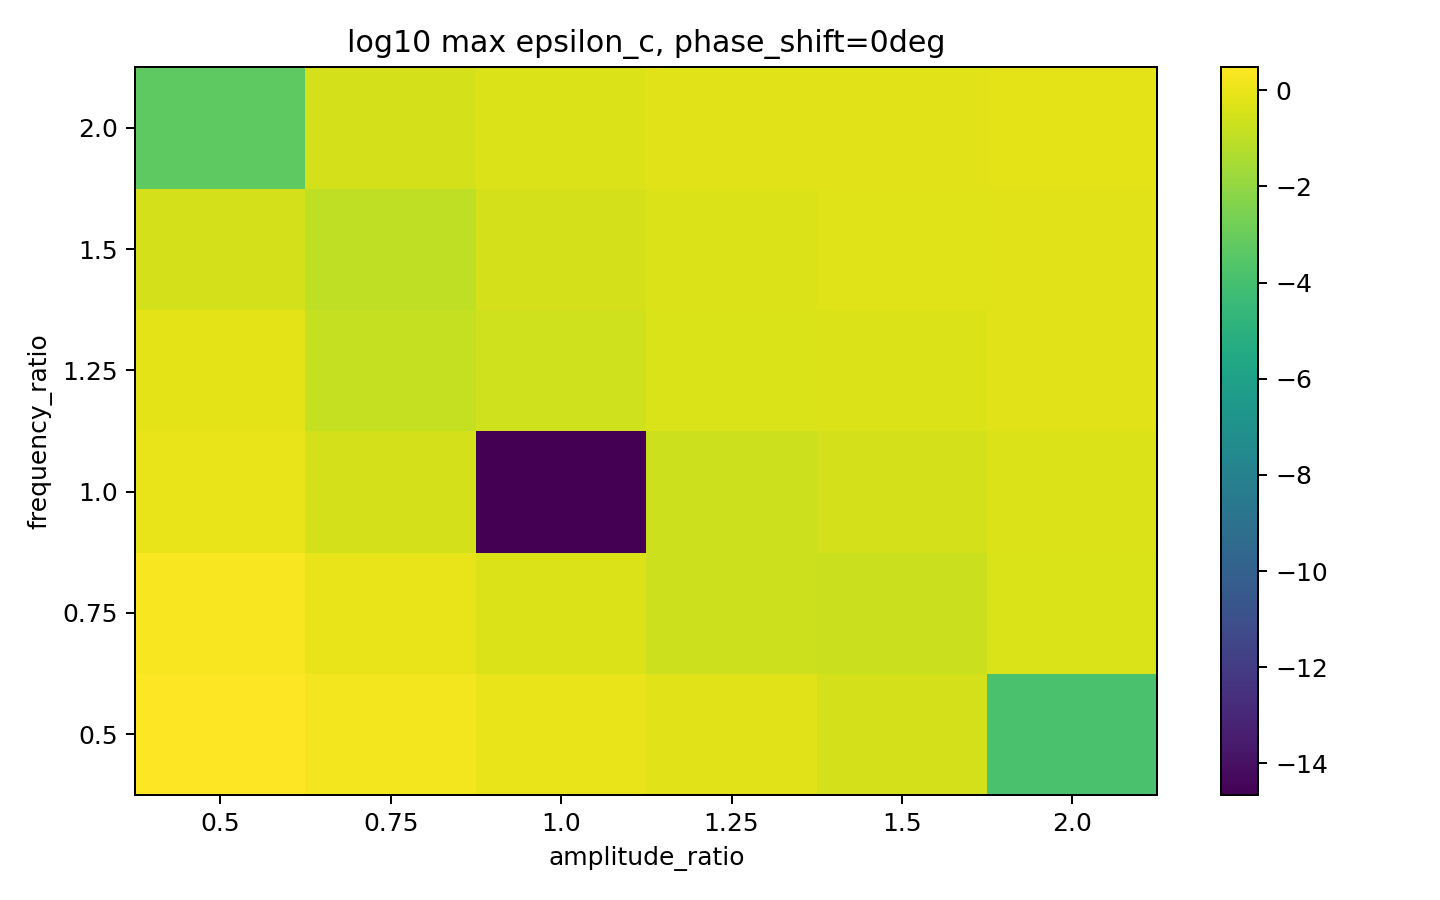
\includegraphics[width=0.45\linewidth,height=\textheight,keepaspectratio,alt={figure}]{ab_two_body_c1_internal_calibration_parameter_sweep_preliminary_result_v1/ab_two_body_c1_parameter_sweep_c_error_heatmap_v1.png}
&
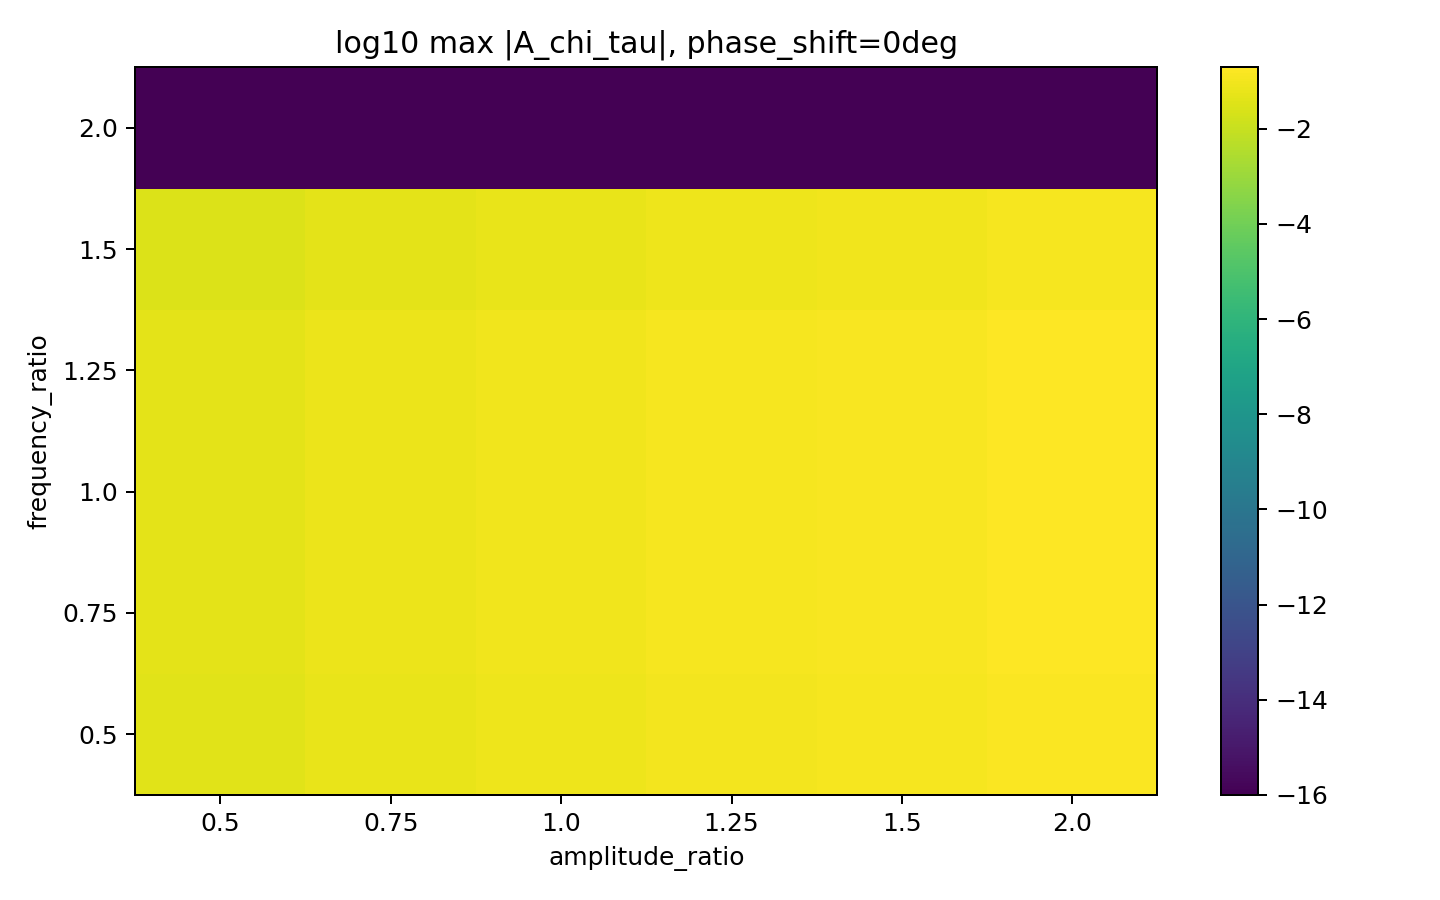
\includegraphics[width=0.45\linewidth,height=\textheight,keepaspectratio,alt={figure}]{ab_two_body_c1_internal_calibration_parameter_sweep_preliminary_result_v1/ab_two_body_c1_parameter_sweep_area_heatmap_v1.png} \\
\end{longtable}
}

{\def\LTcaptype{none} % do not increment counter
\begin{longtable}[]{@{}
  >{\raggedright\arraybackslash}p{(\linewidth - 2\tabcolsep) * \real{0.5000}}
  >{\raggedright\arraybackslash}p{(\linewidth - 2\tabcolsep) * \real{0.5000}}@{}}
\toprule\noalign{}
\begin{minipage}[b]{\linewidth}\raggedright
位相差応答
\end{minipage} & \begin{minipage}[b]{\linewidth}\raggedright
読出しリーク
\end{minipage} \\
\midrule\noalign{}
\endhead
\bottomrule\noalign{}
\endlastfoot
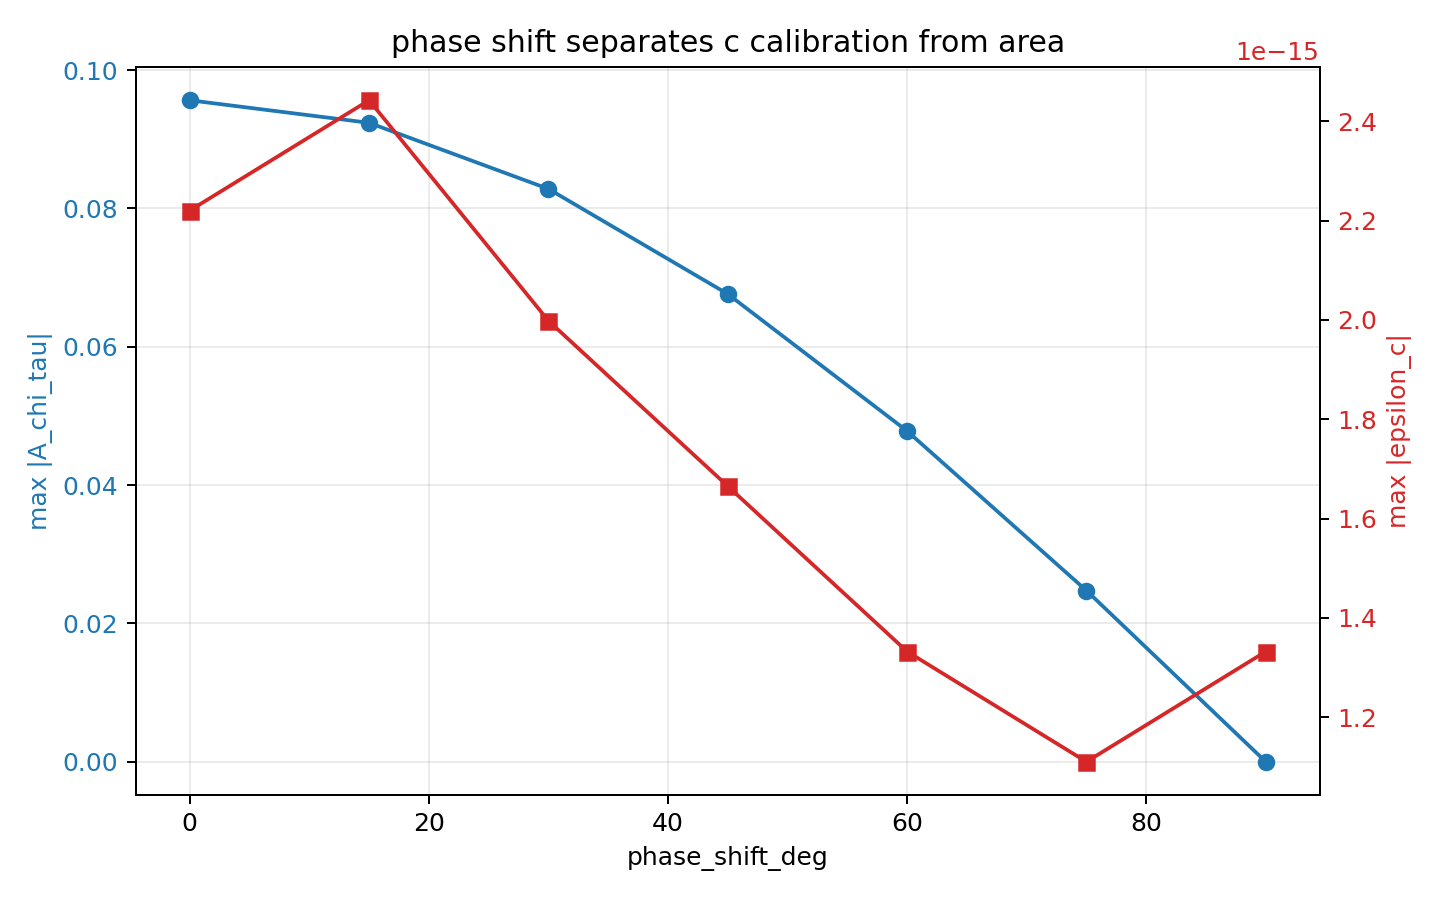
\includegraphics[width=0.45\linewidth,height=\textheight,keepaspectratio,alt={figure}]{ab_two_body_c1_internal_calibration_parameter_sweep_preliminary_result_v1/ab_two_body_c1_parameter_sweep_phase_response_v1.png}
&
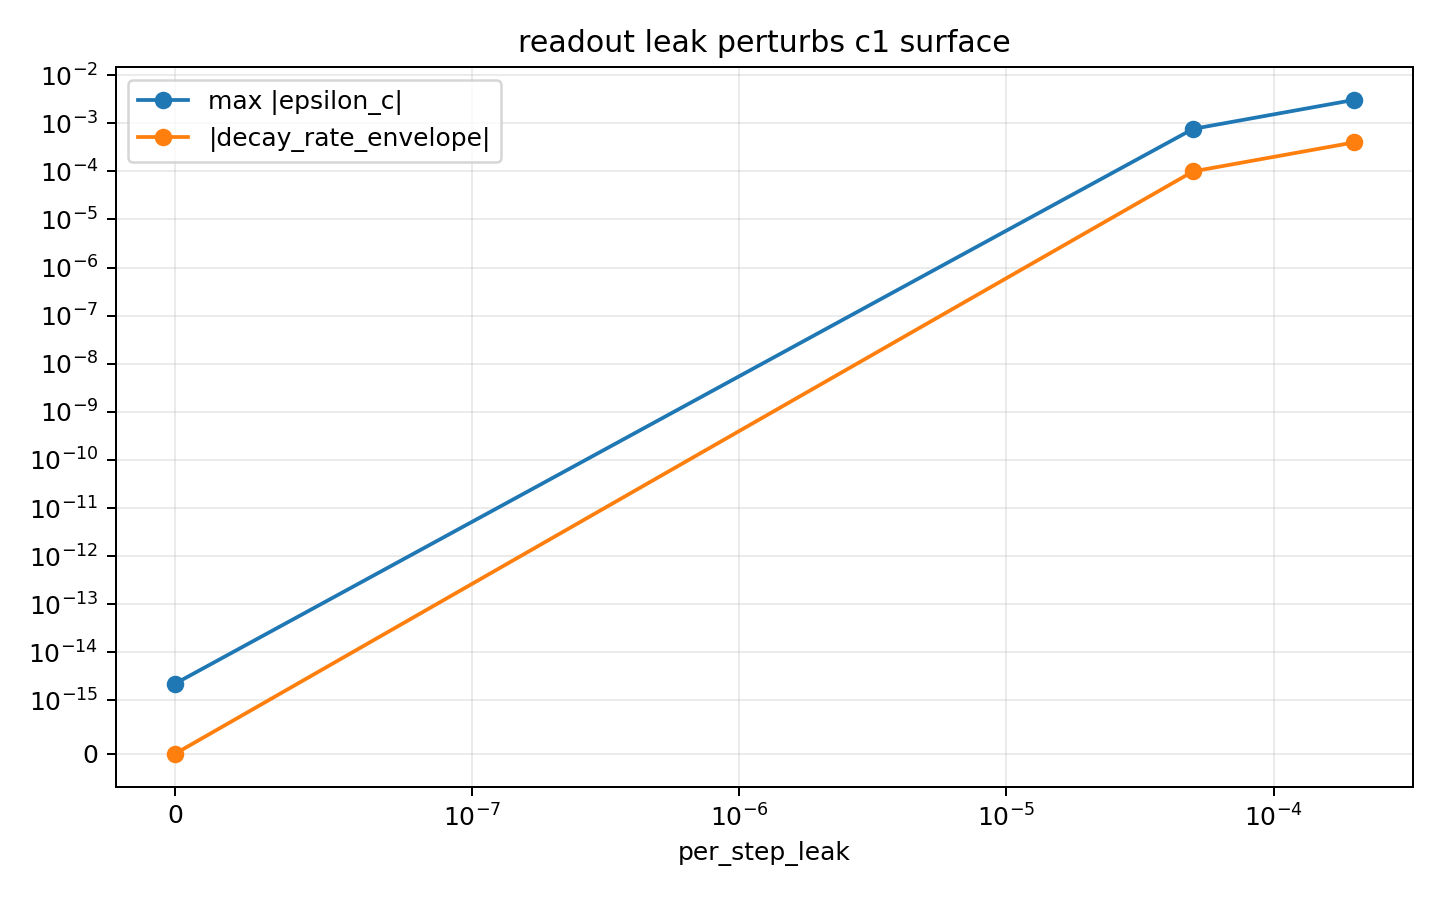
\includegraphics[width=0.45\linewidth,height=\textheight,keepaspectratio,alt={figure}]{ab_two_body_c1_internal_calibration_parameter_sweep_preliminary_result_v1/ab_two_body_c1_parameter_sweep_readout_leak_v1.png} \\
\end{longtable}
}

\begin{center}\rule{0.5\linewidth}{0.5pt}\end{center}

\subsection{6.
逆面積補償診断}\label{ux9006ux9762ux7a4dux88dcux511fux8a3aux65ad}

\subsubsection{6.1 目的}\label{ux76eeux7684}

\texttt{chi-tau} 面積が成立した後、

\begin{Shaded}
\begin{Highlighting}[]
\NormalTok{1 / A\_chi\_tau}
\end{Highlighting}
\end{Shaded}

が閉鎖補償側に自然に残るかを検査した。

重要なのは、\texttt{1/A\_chi\_tau} を後処理で作ることではない。

それは構成済み対照であり、native readout とは区別する。

\subsubsection{6.2 主結果}\label{ux4e3bux7d50ux679c-4}

{\def\LTcaptype{none} % do not increment counter
\begin{longtable}[]{@{}lr@{}}
\toprule\noalign{}
量 & 値 \\
\midrule\noalign{}
\endhead
\bottomrule\noalign{}
\endlastfoot
\texttt{diagnostic\_case\_count} & \texttt{288} \\
\texttt{area\_valid\_case\_count} & \texttt{144} \\
\texttt{fit\_count} & \texttt{576} \\
\texttt{native\_fit\_count} & \texttt{132} \\
\texttt{derived\_fit\_count} & \texttt{84} \\
\texttt{native\_positive2\_count} & \texttt{0} \\
\texttt{constructed\_reciprocal\_positive2\_count} & \texttt{2} \\
\end{longtable}
}

結果は明確である。

\begin{Shaded}
\begin{Highlighting}[]
\NormalTok{1 / A\_chi\_tau を作れば alpha≈2 になる。}
\NormalTok{しかし native readout には alpha≈2 は出ていない。}
\end{Highlighting}
\end{Shaded}

{\def\LTcaptype{none} % do not increment counter
\begin{longtable}[]{@{}
  >{\raggedright\arraybackslash}p{(\linewidth - 2\tabcolsep) * \real{0.5000}}
  >{\raggedright\arraybackslash}p{(\linewidth - 2\tabcolsep) * \real{0.5000}}@{}}
\toprule\noalign{}
\begin{minipage}[b]{\linewidth}\raggedright
構成済み逆面積対照
\end{minipage} & \begin{minipage}[b]{\linewidth}\raggedright
native 候補
\end{minipage} \\
\midrule\noalign{}
\endhead
\bottomrule\noalign{}
\endlastfoot
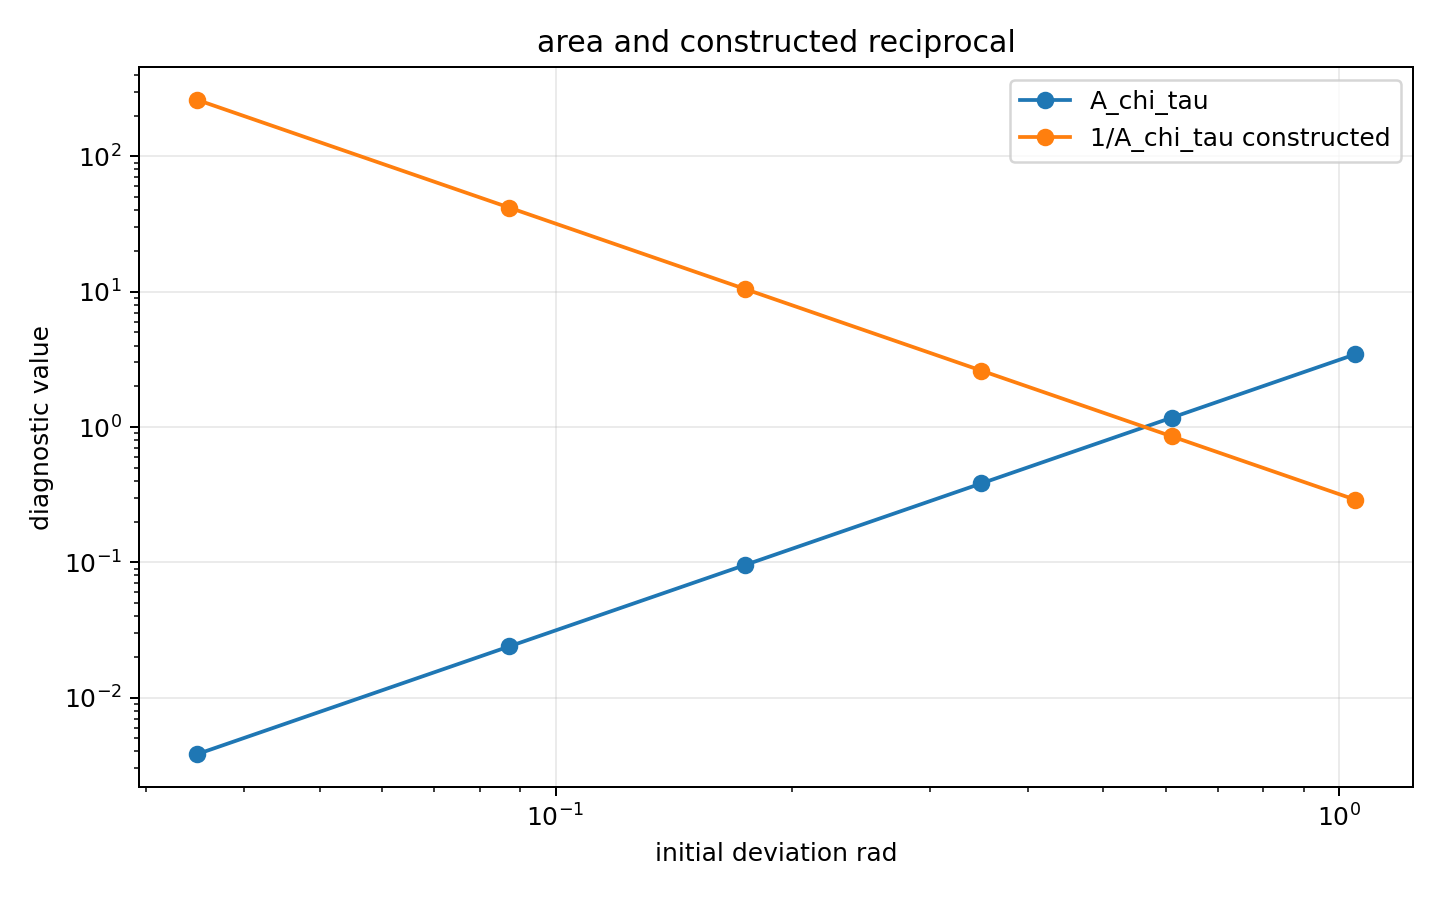
\includegraphics[width=0.45\linewidth,height=\textheight,keepaspectratio,alt={figure}]{ab_two_body_chi_tau_inverse_area_compensation_diagnostic_preliminary_result_v1/ab_two_body_chi_tau_inverse_area_constructed_control_v1.png}
&
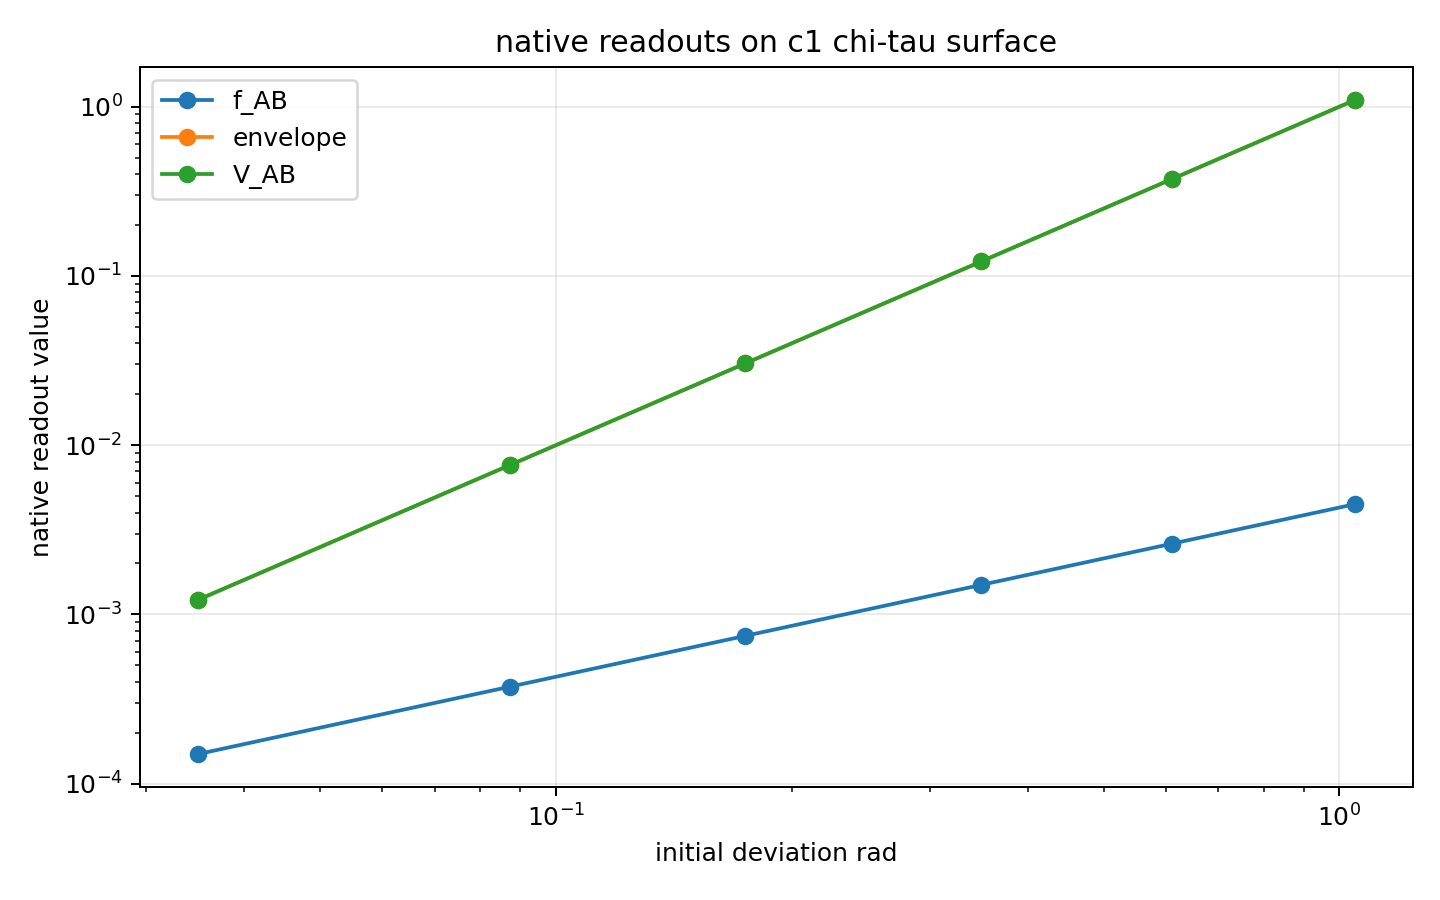
\includegraphics[width=0.45\linewidth,height=\textheight,keepaspectratio,alt={figure}]{ab_two_body_chi_tau_inverse_area_compensation_diagnostic_preliminary_result_v1/ab_two_body_chi_tau_inverse_area_native_candidates_v1.png} \\
\end{longtable}
}

{\def\LTcaptype{none} % do not increment counter
\begin{longtable}[]{@{}
  >{\raggedright\arraybackslash}p{(\linewidth - 0\tabcolsep) * \real{1.0000}}@{}}
\toprule\noalign{}
\begin{minipage}[b]{\linewidth}\raggedright
alpha 比較
\end{minipage} \\
\midrule\noalign{}
\endhead
\bottomrule\noalign{}
\endlastfoot
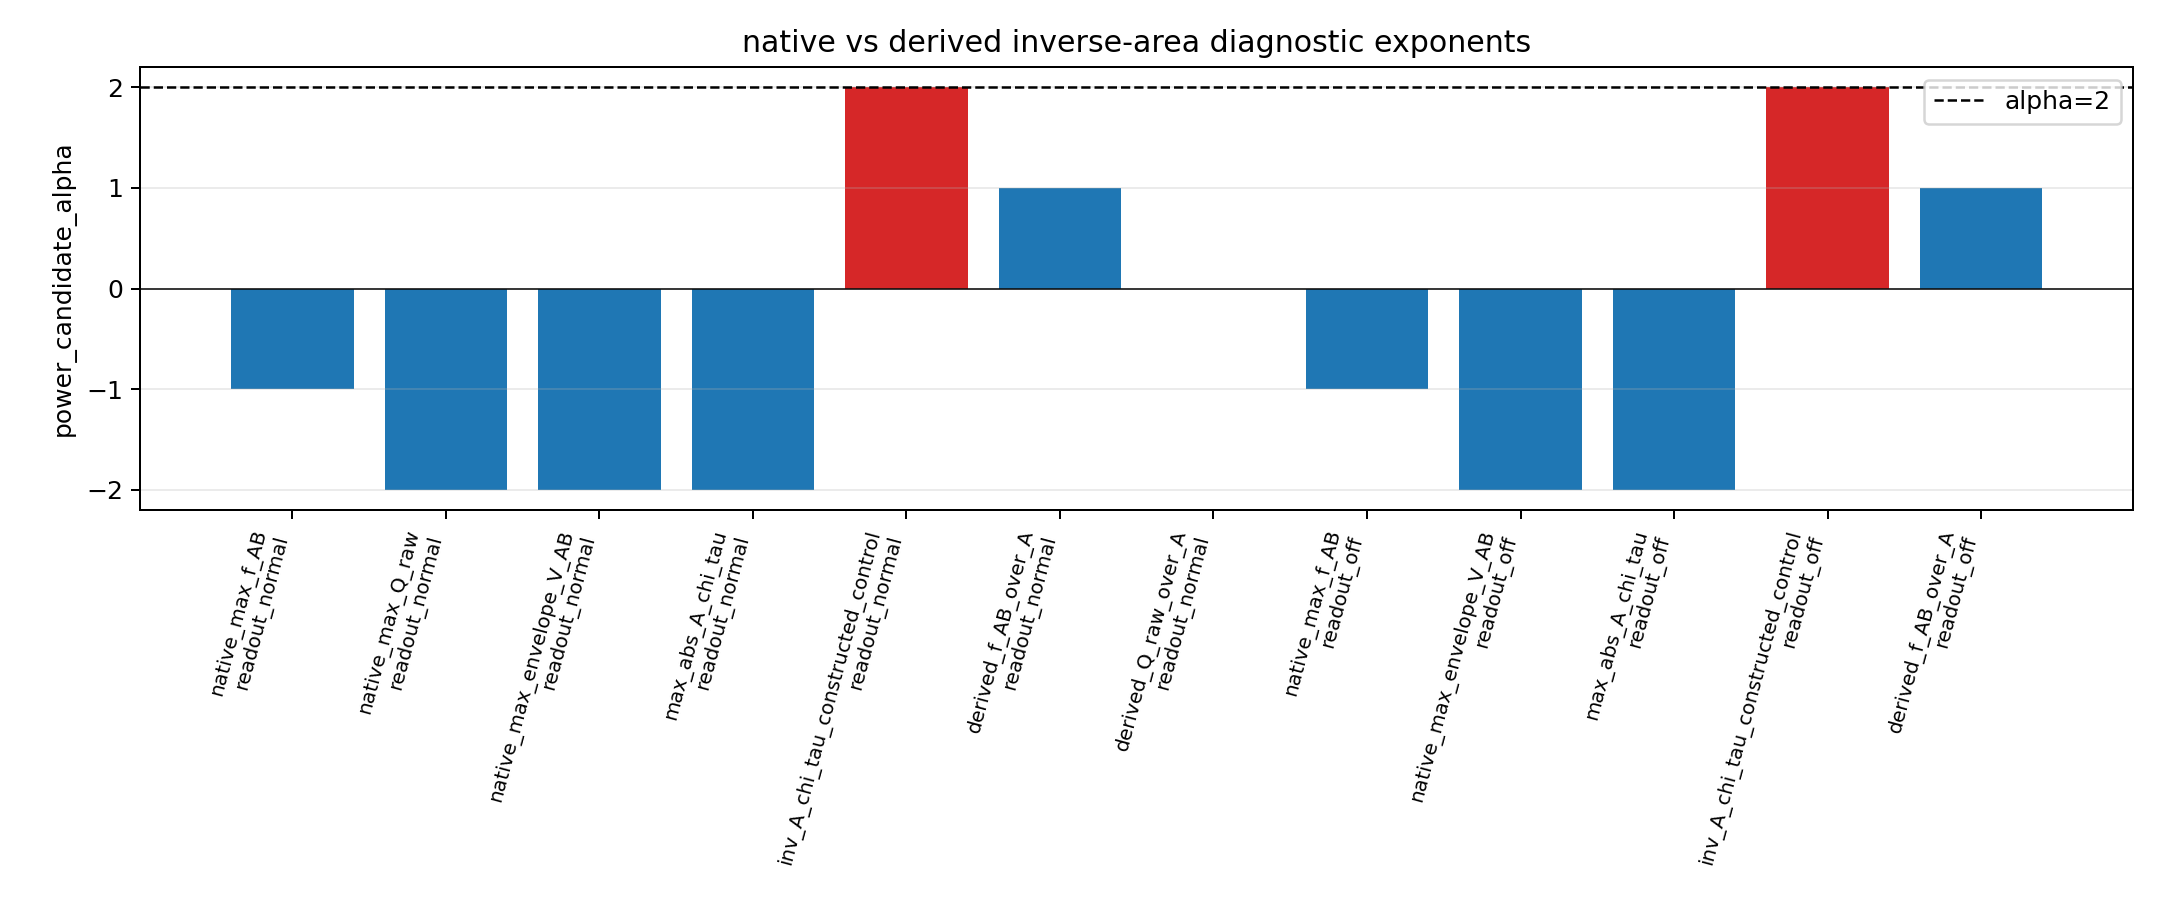
\includegraphics[width=0.65\linewidth,height=\textheight,keepaspectratio,alt={figure}]{ab_two_body_chi_tau_inverse_area_compensation_diagnostic_preliminary_result_v1/ab_two_body_chi_tau_inverse_area_alpha_comparison_v1.png} \\
\end{longtable}
}

\begin{center}\rule{0.5\linewidth}{0.5pt}\end{center}

\subsection{7.
native逆面積拡張スイープ}\label{nativeux9006ux9762ux7a4dux62e1ux5f35ux30b9ux30a4ux30fcux30d7}

\subsubsection{7.1 主結果}\label{ux4e3bux7d50ux679c-5}

{\def\LTcaptype{none} % do not increment counter
\begin{longtable}[]{@{}lr@{}}
\toprule\noalign{}
量 & 値 \\
\midrule\noalign{}
\endhead
\bottomrule\noalign{}
\endlastfoot
\texttt{sweep\_case\_count} & \texttt{1323} \\
\texttt{area\_valid\_case\_count} & \texttt{1260} \\
\texttt{c1\_surface\_like\_case\_count} & \texttt{126} \\
\texttt{fit\_count} & \texttt{4158} \\
\texttt{native\_fit\_count} & \texttt{1056} \\
\texttt{native\_positive2\_count} & \texttt{0} \\
\texttt{c1\_native\_positive2\_count} & \texttt{0} \\
\texttt{constructed\_reciprocal\_positive2\_count} & \texttt{198} \\
\end{longtable}
}

広いパラメータ範囲でも、

\begin{Shaded}
\begin{Highlighting}[]
\NormalTok{native inverse{-}area scaling は未検出}
\end{Highlighting}
\end{Shaded}

であった。

一方で、構成済み対照では \texttt{alpha≈2} が出る。

したがって、今回の境界は次である。

\begin{Shaded}
\begin{Highlighting}[]
\NormalTok{逆二乗は作れる。}
\NormalTok{しかし、まだ読まれていない。}
\end{Highlighting}
\end{Shaded}

{\def\LTcaptype{none} % do not increment counter
\begin{longtable}[]{@{}
  >{\raggedright\arraybackslash}p{(\linewidth - 2\tabcolsep) * \real{0.5000}}
  >{\raggedright\arraybackslash}p{(\linewidth - 2\tabcolsep) * \real{0.5000}}@{}}
\toprule\noalign{}
\begin{minipage}[b]{\linewidth}\raggedright
参照曲線
\end{minipage} & \begin{minipage}[b]{\linewidth}\raggedright
alpha scan
\end{minipage} \\
\midrule\noalign{}
\endhead
\bottomrule\noalign{}
\endlastfoot
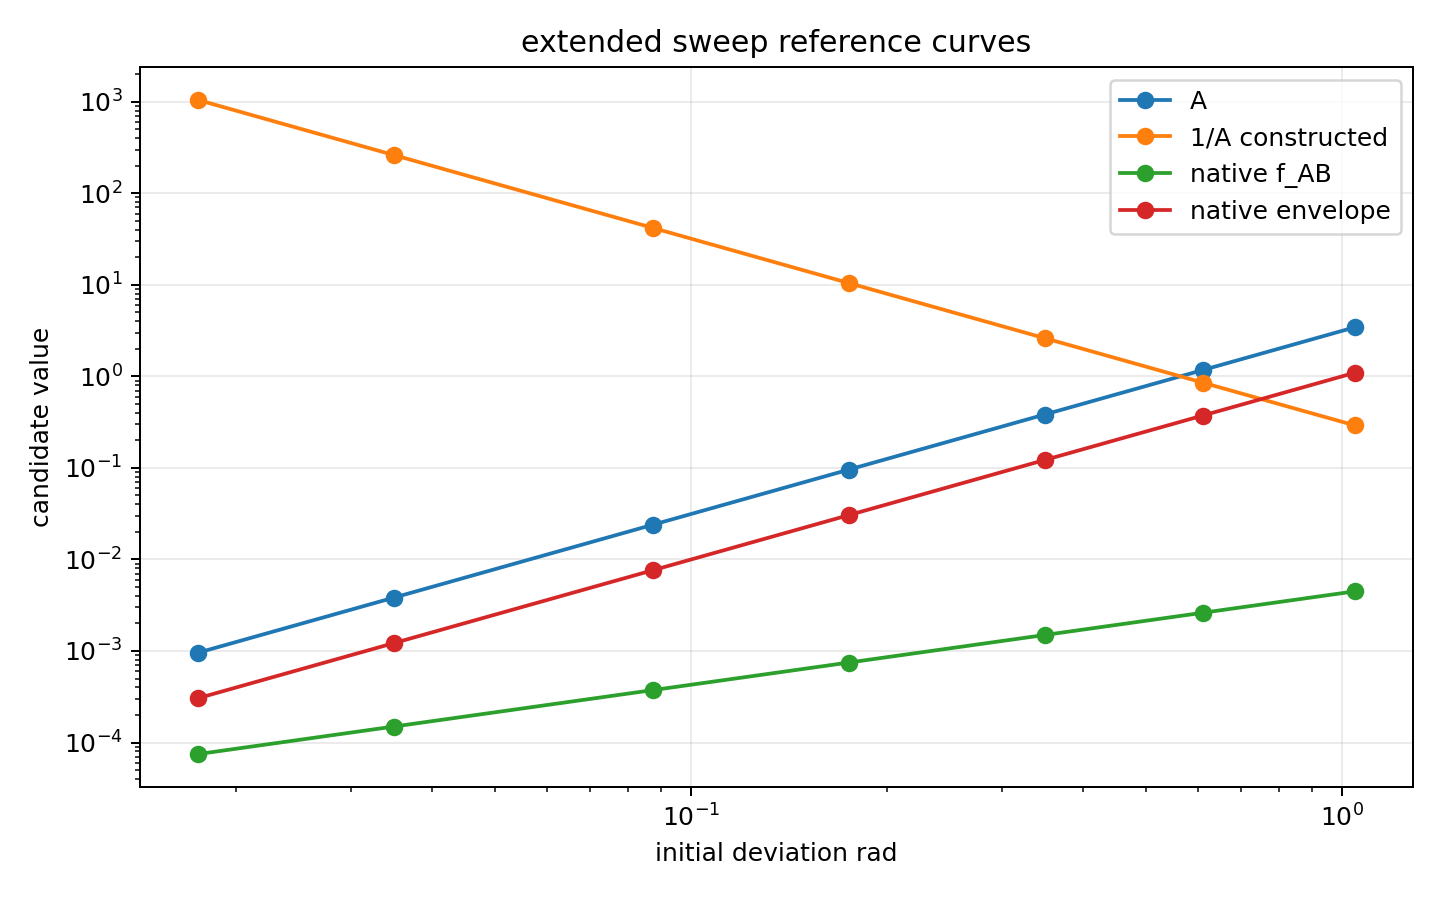
\includegraphics[width=0.45\linewidth,height=\textheight,keepaspectratio,alt={figure}]{ab_two_body_chi_tau_native_inverse_area_extended_sweep_preliminary_result_v1/ab_two_body_native_inverse_area_extended_reference_curves_v1.png}
&
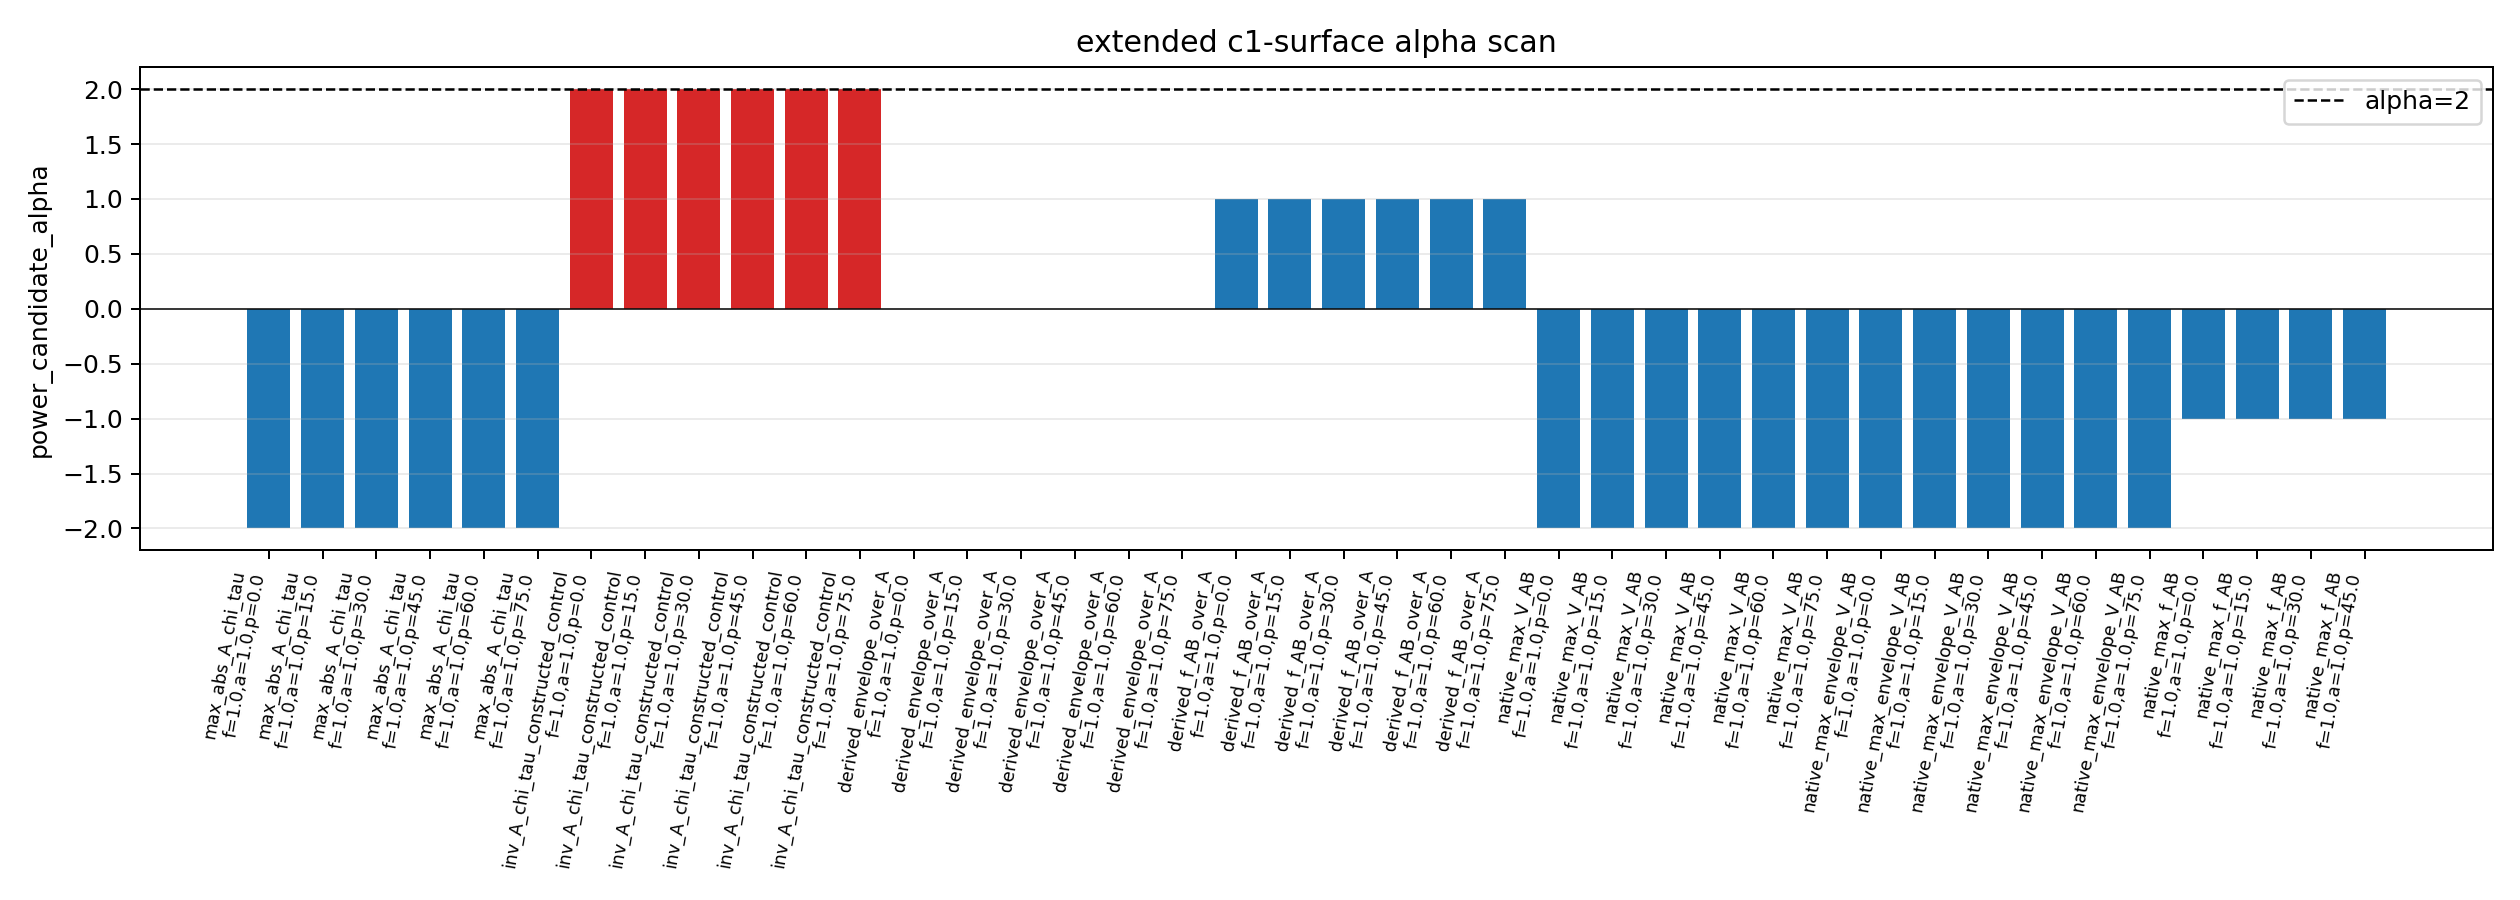
\includegraphics[width=0.45\linewidth,height=\textheight,keepaspectratio,alt={figure}]{ab_two_body_chi_tau_native_inverse_area_extended_sweep_preliminary_result_v1/ab_two_body_native_inverse_area_extended_alpha_scan_v1.png} \\
\end{longtable}
}

\begin{center}\rule{0.5\linewidth}{0.5pt}\end{center}

\subsection{8. V2追加:
フェルミオン型反跳を組み込んだ調和読出し}\label{v2ux8ffdux52a0-ux30d5ux30a7ux30ebux30dfux30aaux30f3ux578bux53cdux8df3ux3092ux7d44ux307fux8fbcux3093ux3060ux8abfux548cux8aadux51faux3057}

\subsubsection{8.1 目的}\label{ux76eeux7684-1}

V1の一角度調和読出しでは、AB二体の相対位相発展を連続的に読み、ラベルなし読出しとして
Protocol F/B が縮退することを確認した。

V2では、この文脈を変えず、中心近傍の相互作用にフェルミオン型反跳写像を組み込む。

ここで検査するのは、反跳写像を入れた場合にも、AB二体関係 \texttt{f\_AB}
から加速度様に見える調和読出しを同じ形式で評価できるかである。

本節では、次を扱わない。

\begin{Shaded}
\begin{Highlighting}[]
\NormalTok{ABの非対称化}
\NormalTok{低局在性極限}
\NormalTok{即時収縮}
\NormalTok{倍音移乗}
\NormalTok{局在性移乗}
\end{Highlighting}
\end{Shaded}

これらは、別系列の波束集束実験で扱う。

本V2では、あくまで現在のAB二体加速度読出しの仮定範囲で、通過型の中心読出しに加えて、フェルミオン型反跳プロトコルを追加する。

\subsubsection{8.2 反跳写像}\label{ux53cdux8df3ux5199ux50cf}

右向き入射チャネルと左向き入射チャネルを、

\begin{Shaded}
\begin{Highlighting}[]
\NormalTok{\textbackslash{}Psi\^{}\{\textbackslash{}mathrm\{in\}\}}
\NormalTok{=}
\NormalTok{\textbackslash{}begin\{pmatrix\}}
\NormalTok{\textbackslash{}psi\_+\^{}\{\textbackslash{}mathrm\{in\}\}\textbackslash{}\textbackslash{}}
\NormalTok{\textbackslash{}psi\_{-}\^{}\{\textbackslash{}mathrm\{in\}\}}
\NormalTok{\textbackslash{}end\{pmatrix\}}
\end{Highlighting}
\end{Shaded}

とする。

フェルミオン型交換位相を \texttt{Delta\_F} とし、透過振幅と反射振幅を、

\begin{Shaded}
\begin{Highlighting}[]
\NormalTok{t\_\textbackslash{}Delta}
\NormalTok{=}
\NormalTok{e\^{}\{i\textbackslash{}Delta\_F/2\}}
\NormalTok{\textbackslash{}cos\textbackslash{}frac\{\textbackslash{}Delta\_F\}\{2\}}
\end{Highlighting}
\end{Shaded}

\begin{Shaded}
\begin{Highlighting}[]
\NormalTok{r\_\textbackslash{}Delta}
\NormalTok{=}
\NormalTok{{-}i e\^{}\{i\textbackslash{}Delta\_F/2\}}
\NormalTok{\textbackslash{}sin\textbackslash{}frac\{\textbackslash{}Delta\_F\}\{2\}}
\end{Highlighting}
\end{Shaded}

と定義する。

二チャネル散乱行列は、

\begin{Shaded}
\begin{Highlighting}[]
\NormalTok{S\_\textbackslash{}Delta}
\NormalTok{=}
\NormalTok{\textbackslash{}begin\{pmatrix\}}
\NormalTok{t\_\textbackslash{}Delta \& r\_\textbackslash{}Delta\textbackslash{}\textbackslash{}}
\NormalTok{r\_\textbackslash{}Delta \& t\_\textbackslash{}Delta}
\NormalTok{\textbackslash{}end\{pmatrix\}}
\end{Highlighting}
\end{Shaded}

であり、出射チャネルを、

\begin{Shaded}
\begin{Highlighting}[]
\NormalTok{\textbackslash{}Psi\^{}\{\textbackslash{}mathrm\{out\}\}}
\NormalTok{=}
\NormalTok{S\_\textbackslash{}Delta}
\NormalTok{\textbackslash{}Psi\^{}\{\textbackslash{}mathrm\{in\}\}}
\end{Highlighting}
\end{Shaded}

として読む。

すなわち、

\begin{Shaded}
\begin{Highlighting}[]
\NormalTok{\textbackslash{}psi\_+\^{}\{\textbackslash{}mathrm\{out\}\}}
\NormalTok{=}
\NormalTok{t\_\textbackslash{}Delta \textbackslash{}psi\_+\^{}\{\textbackslash{}mathrm\{in\}\}}
\NormalTok{+}
\NormalTok{r\_\textbackslash{}Delta \textbackslash{}psi\_{-}\^{}\{\textbackslash{}mathrm\{in\}\}}
\end{Highlighting}
\end{Shaded}

\begin{Shaded}
\begin{Highlighting}[]
\NormalTok{\textbackslash{}psi\_{-}\^{}\{\textbackslash{}mathrm\{out\}\}}
\NormalTok{=}
\NormalTok{r\_\textbackslash{}Delta \textbackslash{}psi\_+\^{}\{\textbackslash{}mathrm\{in\}\}}
\NormalTok{+}
\NormalTok{t\_\textbackslash{}Delta \textbackslash{}psi\_{-}\^{}\{\textbackslash{}mathrm\{in\}\}}
\end{Highlighting}
\end{Shaded}

である。

完全反跳条件では、

\begin{Shaded}
\begin{Highlighting}[]
\NormalTok{\textbackslash{}Delta\_F=\textbackslash{}pi}
\end{Highlighting}
\end{Shaded}

であり、

\begin{Shaded}
\begin{Highlighting}[]
\NormalTok{透過振幅 t\_Delta = 0}
\NormalTok{反射振幅 r\_Delta = 1}
\end{Highlighting}
\end{Shaded}

に相当する。

このとき、出射チャネルは入射チャネルの交換として読まれる。

\subsubsection{8.3
実験前の判定基準}\label{ux5b9fux9a13ux524dux306eux5224ux5b9aux57faux6e96}

V2追加プロトコルでは、少なくとも次を確認する。

{\def\LTcaptype{none} % do not increment counter
\begin{longtable}[]{@{}
  >{\raggedright\arraybackslash}p{(\linewidth - 2\tabcolsep) * \real{0.5000}}
  >{\raggedright\arraybackslash}p{(\linewidth - 2\tabcolsep) * \real{0.5000}}@{}}
\toprule\noalign{}
\begin{minipage}[b]{\linewidth}\raggedright
項目
\end{minipage} & \begin{minipage}[b]{\linewidth}\raggedright
判定対象
\end{minipage} \\
\midrule\noalign{}
\endhead
\bottomrule\noalign{}
\endlastfoot
反跳後の閉鎖残差 & \texttt{Q\_closed} が破綻しないこと \\
調和読出し & \texttt{D\_AB}, \texttt{V\_AB}, \texttt{f\_AB}
の調和構造が維持されること \\
読出し漏れ応答 & 読出し停止時と強読出し時の差がV1と同じ規律を持つこと \\
Protocol比較 &
通過型・表示反跳型・フェルミオン型反跳型の差分が記録されること \\
\texttt{chi-tau} 面 & 独立 \texttt{tau\_read}
による面積読出しを壊さないこと \\
\end{longtable}
}

\subsubsection{8.4 主結果}\label{ux4e3bux7d50ux679c-6}

{\def\LTcaptype{none} % do not increment counter
\begin{longtable}[]{@{}
  >{\raggedright\arraybackslash}p{(\linewidth - 2\tabcolsep) * \real{0.4286}}
  >{\raggedleft\arraybackslash}p{(\linewidth - 2\tabcolsep) * \real{0.5714}}@{}}
\toprule\noalign{}
\begin{minipage}[b]{\linewidth}\raggedright
量
\end{minipage} & \begin{minipage}[b]{\linewidth}\raggedleft
値
\end{minipage} \\
\midrule\noalign{}
\endhead
\bottomrule\noalign{}
\endlastfoot
\texttt{harmonic\_case\_count} & \texttt{48} \\
\texttt{c1\_case\_count} & \texttt{144} \\
\texttt{scattering\_protocol\_count} & \texttt{3} \\
\texttt{fermionic\_delta\_f} & \texttt{3.141592653589793} \\
\texttt{fermionic\_reflection\_rate} & \texttt{1.0} \\
\texttt{fermionic\_transmission\_rate} &
\texttt{3.749399456654644e-33} \\
\texttt{fermionic\_q\_out\_factor} & \texttt{-1.0} \\
\texttt{max\_Q\_closed\_abs} & \texttt{0.0} \\
\texttt{fermionic\_regular\_cell\_harmonic\_consistent\_nonstrong\_modes}
& \texttt{True} \\
\texttt{fermionic\_strong\_readout\_perturbs\_harmonic\_projection} &
\texttt{True} \\
\texttt{fermionic\_max\_f\_AB\_projection\_error\_regular\_nonstrong} &
\texttt{2.2756072064285173e-6} \\
\texttt{fermionic\_max\_f\_AB\_projection\_error\_regular\_strong} &
\texttt{9.072436576166722e-6} \\
\texttt{fermionic\_reflection\_event\_cell\_count\_total} &
\texttt{720} \\
\texttt{label\_free\_pass\_vs\_fermionic\_match\_all\_cases} &
\texttt{True} \\
\texttt{label\_free\_display\_vs\_fermionic\_match\_all\_cases} &
\texttt{True} \\
\texttt{readout\_off\_decay\_max\_abs} &
\texttt{4.4544900995234305e-18} \\
\texttt{readout\_strong\_decay\_min\_abs} &
\texttt{4.0004000533409075e-4} \\
\texttt{fermionic\_tau\_disabled\_max\_area} & \texttt{0.0} \\
\texttt{fermionic\_tau\_locked\_max\_area} & \texttt{0.0} \\
\texttt{fermionic\_tau\_independent\_min\_area} &
\texttt{0.00375268307733001} \\
\texttt{fermionic\_c1\_readout\_off\_max\_epsilon\_c\_abs} &
\texttt{2.3314683517128287e-15} \\
\texttt{fermionic\_c1\_area\_sweep\_detected\_all\_cases} &
\texttt{True} \\
\texttt{tau\_is\_step\_used\_any} & \texttt{False} \\
\texttt{external\_c\_used\_any} & \texttt{False} \\
\texttt{f\_A\_or\_f\_B\_used\_any} & \texttt{False} \\
\end{longtable}
}

結果は次のように読める。

\begin{Shaded}
\begin{Highlighting}[]
\NormalTok{フェルミオン型反跳写像は、}
\NormalTok{Delta\_F = pi において R=1, T≈0, q\_out\_factor={-}1 を与えた。}
\end{Highlighting}
\end{Shaded}

また、フェルミオン型反跳は座標の折返し表示ではなく、出射チャネル交換として実装した。

そのため、ラベルなし読出し \texttt{D\_AB}, \texttt{V\_AB}
は、V1の通過型読出しと一致した。

これは、V1で確認した Protocol F/B 縮退と整合する。

一方で、表示上だけ折り返す \texttt{display\_reflection}
も対照として記録した。

この表示反跳とフェルミオン型反跳も、ラベルなし \texttt{D\_AB},
\texttt{V\_AB} では一致した。

調和読出しについては、V1と同じく、非 \texttt{readout\_strong}
条件では射影整合性が保たれた。

強読出しでは射影歪みが出たが、これはV1の読出し波摂動と同じ性質であり、反跳写像固有の破綻ではない。

\texttt{chi-tau} 面についても、

\begin{Shaded}
\begin{Highlighting}[]
\NormalTok{tau disabled: 面積なし}
\NormalTok{tau locked: 面積なし}
\NormalTok{tau independent c1: 面積あり}
\end{Highlighting}
\end{Shaded}

が維持された。

したがって、フェルミオン型反跳写像をAB二体加速度読出しへ組み込んでも、現在の仮定範囲では、加速度様調和読出しと
\texttt{chi-tau} 面積読出しは壊れない。

\subsubsection{8.5 図}\label{ux56f3-2}

{\def\LTcaptype{none} % do not increment counter
\begin{longtable}[]{@{}
  >{\raggedright\arraybackslash}p{(\linewidth - 2\tabcolsep) * \real{0.5000}}
  >{\raggedright\arraybackslash}p{(\linewidth - 2\tabcolsep) * \real{0.5000}}@{}}
\toprule\noalign{}
\begin{minipage}[b]{\linewidth}\raggedright
Protocol 比較
\end{minipage} & \begin{minipage}[b]{\linewidth}\raggedright
チャネル状態
\end{minipage} \\
\midrule\noalign{}
\endhead
\bottomrule\noalign{}
\endlastfoot
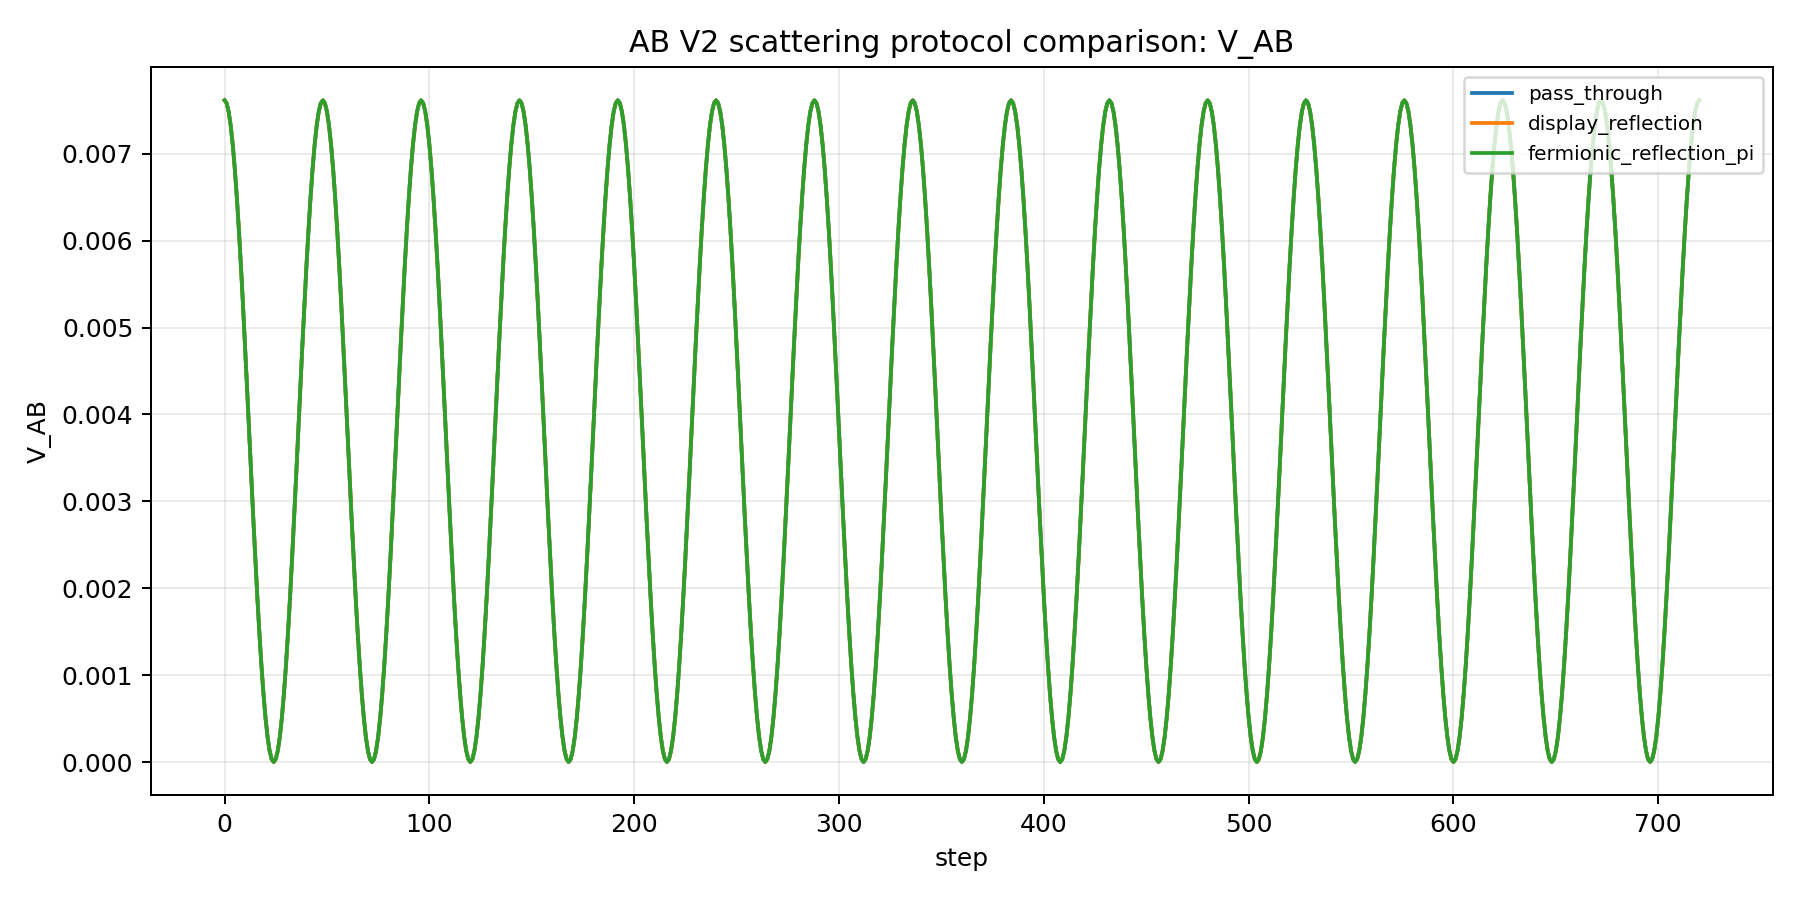
\includegraphics[width=0.45\linewidth,height=\textheight,keepaspectratio,alt={figure}]{ab_two_body_fermionic_reflection_harmonic_readout_preliminary_result_v2/ab_two_body_fermionic_reflection_protocol_comparison_v2.png}
&
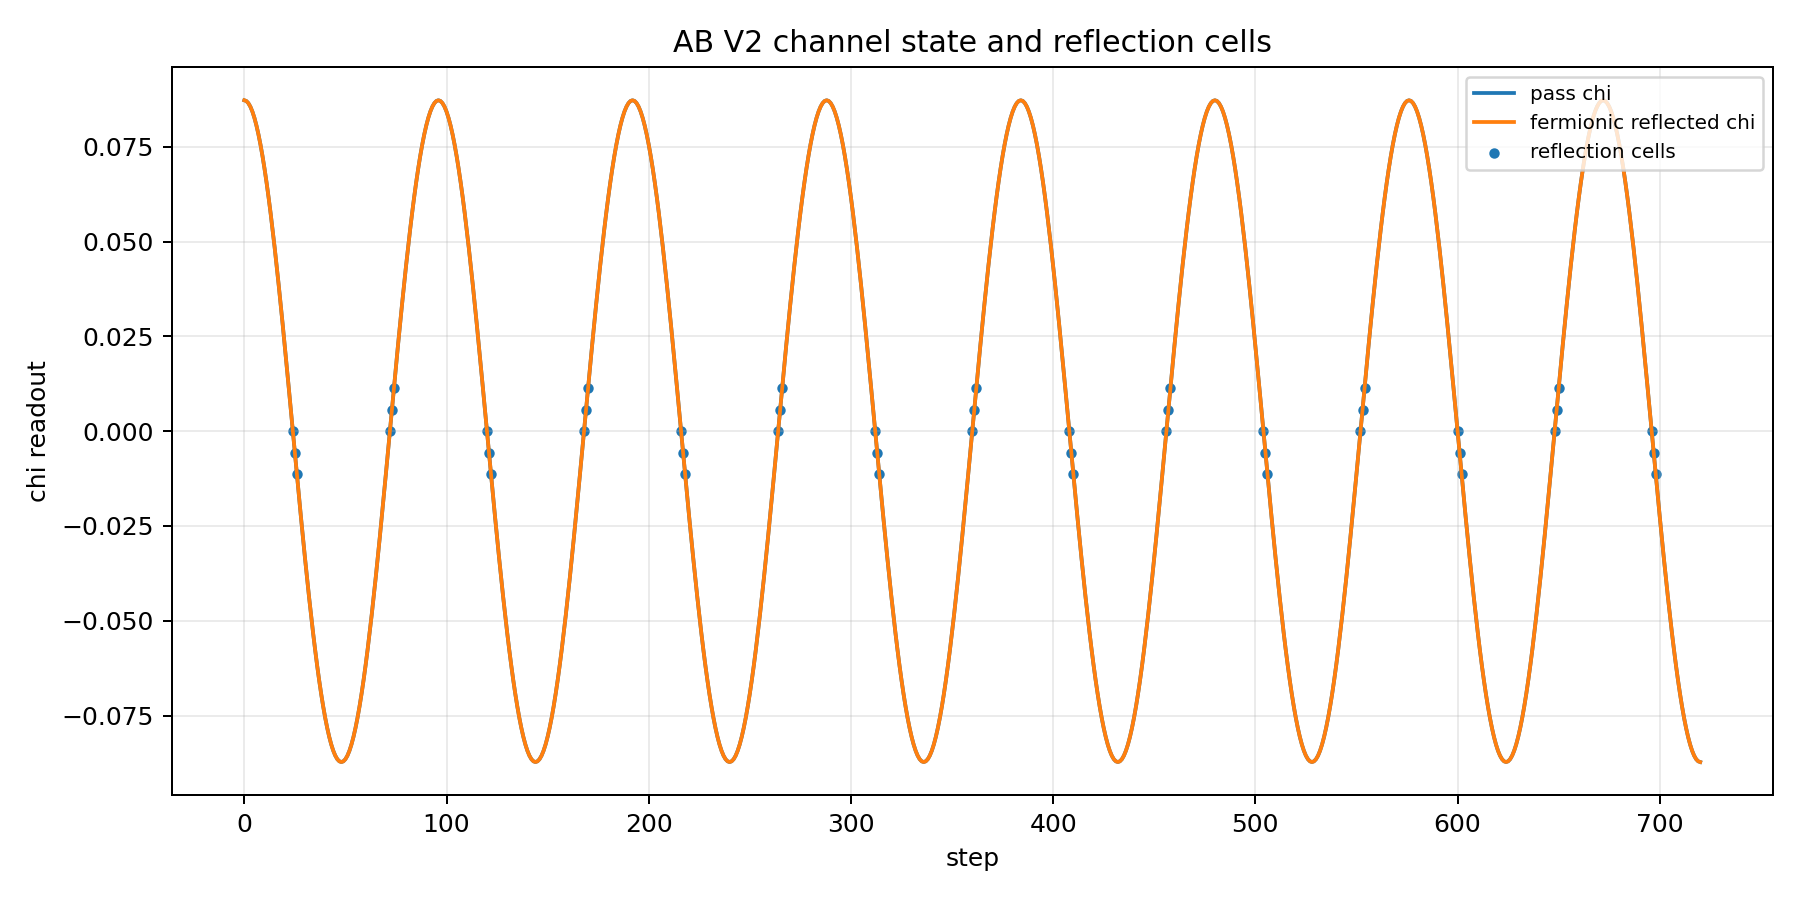
\includegraphics[width=0.45\linewidth,height=\textheight,keepaspectratio,alt={figure}]{ab_two_body_fermionic_reflection_harmonic_readout_preliminary_result_v2/ab_two_body_fermionic_reflection_channel_state_v2.png} \\
\end{longtable}
}

{\def\LTcaptype{none} % do not increment counter
\begin{longtable}[]{@{}
  >{\raggedright\arraybackslash}p{(\linewidth - 2\tabcolsep) * \real{0.5000}}
  >{\raggedright\arraybackslash}p{(\linewidth - 2\tabcolsep) * \real{0.5000}}@{}}
\toprule\noalign{}
\begin{minipage}[b]{\linewidth}\raggedright
読出し減衰
\end{minipage} & \begin{minipage}[b]{\linewidth}\raggedright
\texttt{chi-tau} 経路
\end{minipage} \\
\midrule\noalign{}
\endhead
\bottomrule\noalign{}
\endlastfoot
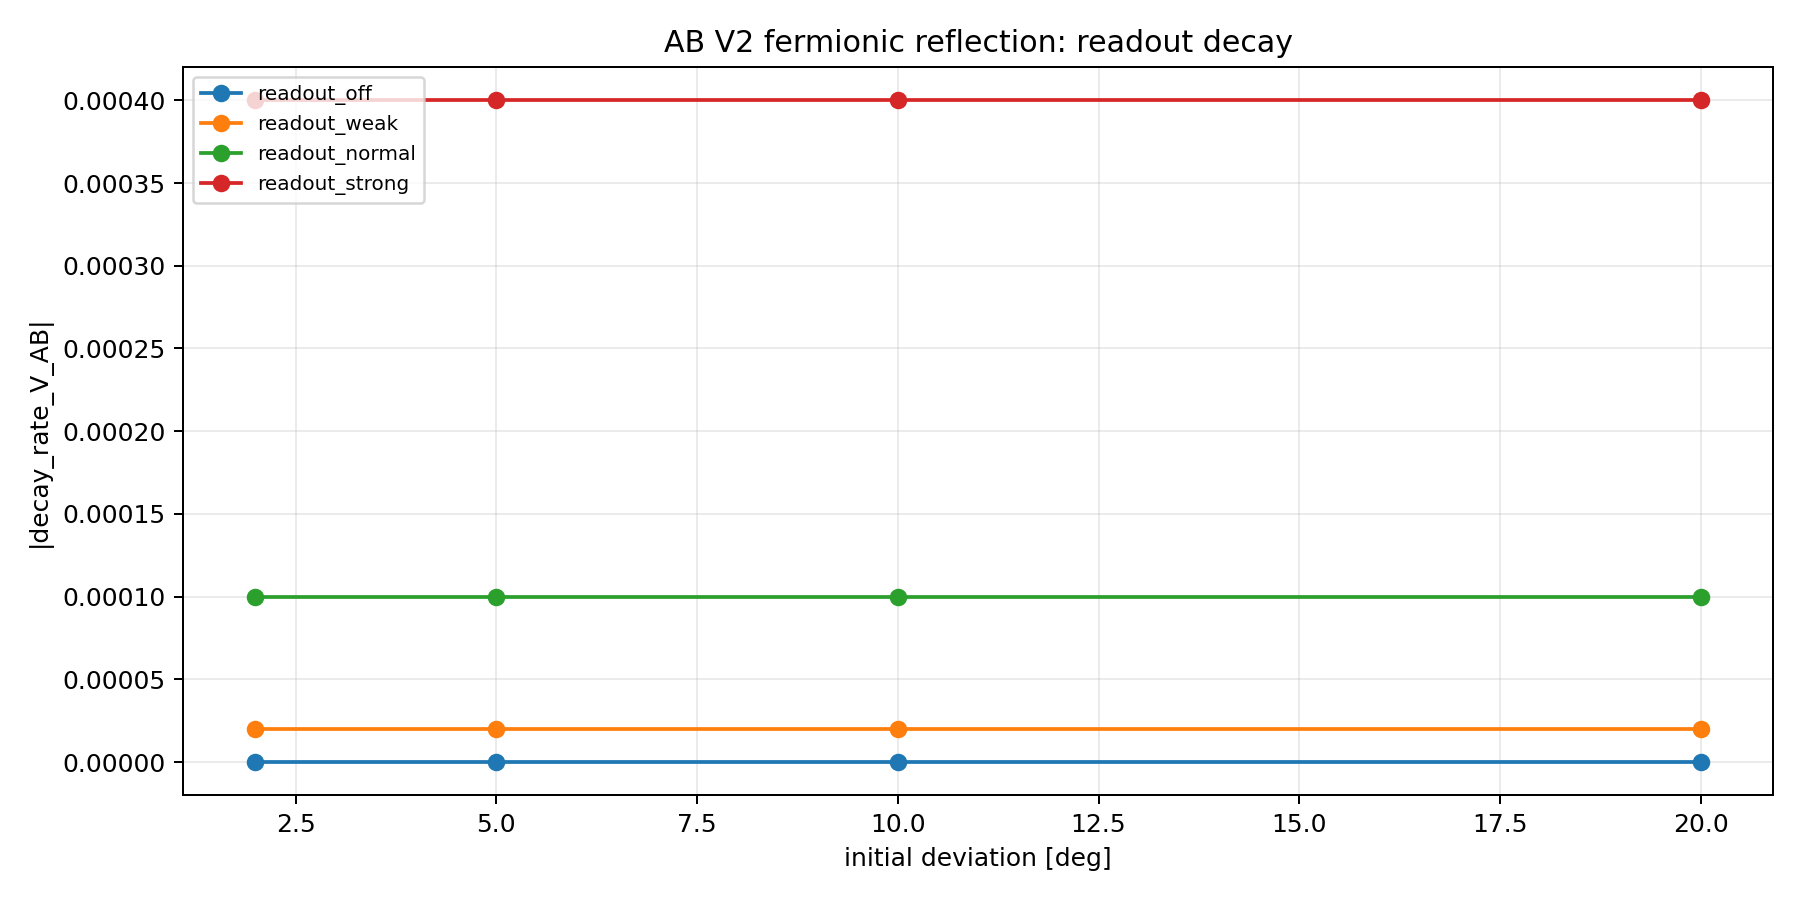
\includegraphics[width=0.45\linewidth,height=\textheight,keepaspectratio,alt={figure}]{ab_two_body_fermionic_reflection_harmonic_readout_preliminary_result_v2/ab_two_body_fermionic_reflection_readout_decay_v2.png}
&
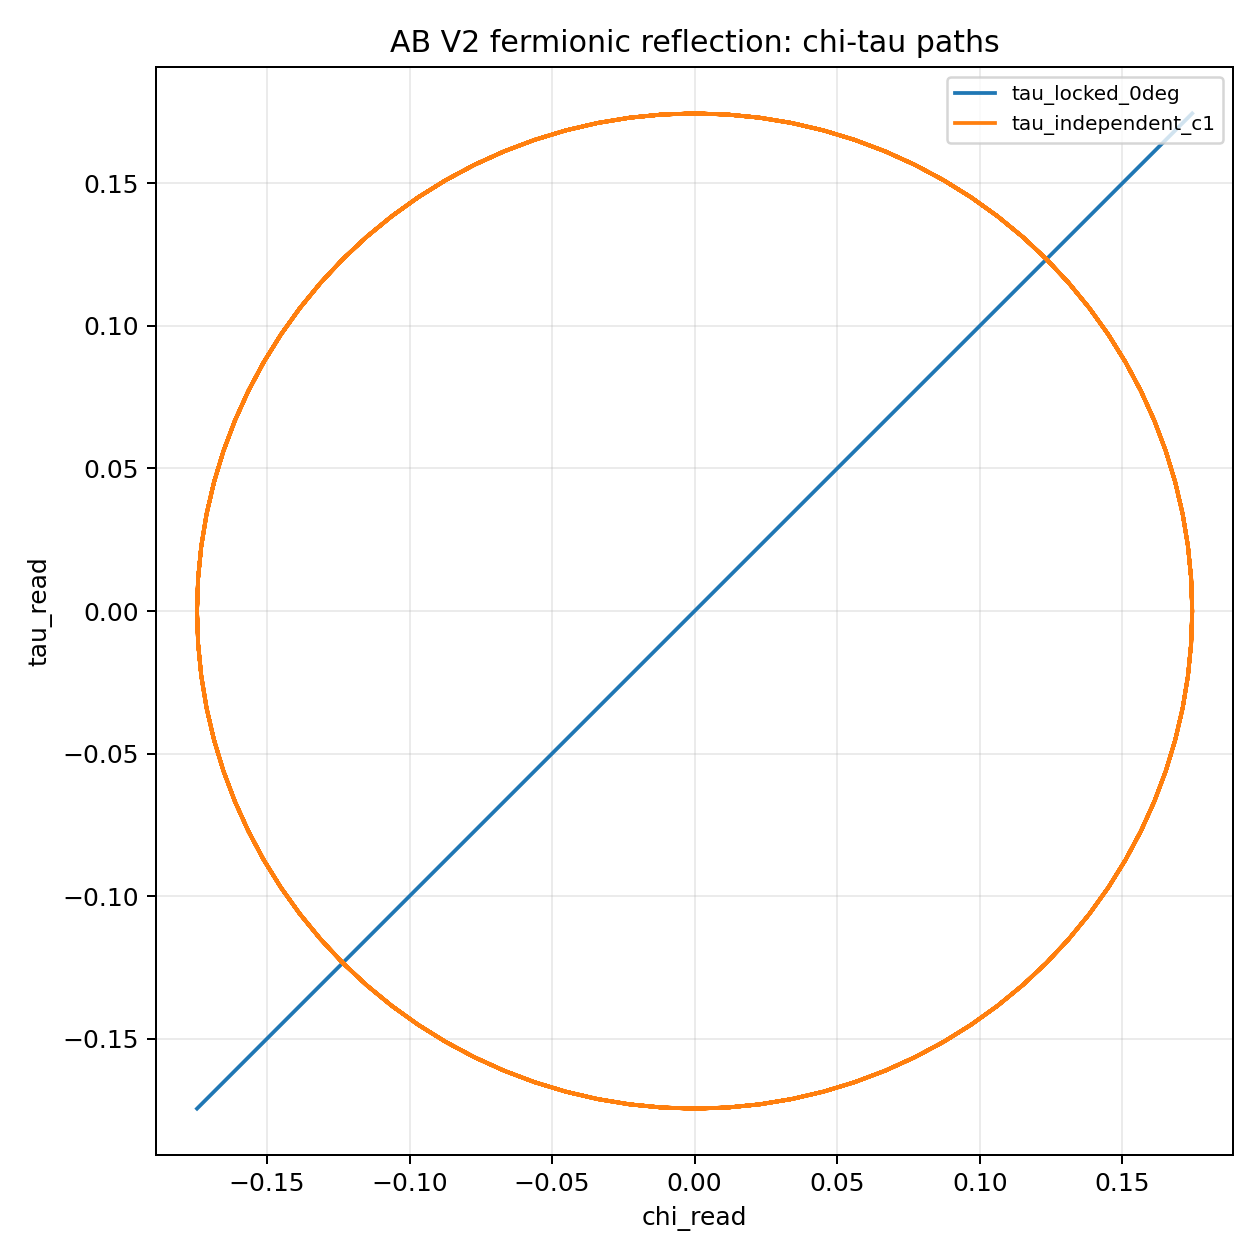
\includegraphics[width=0.45\linewidth,height=\textheight,keepaspectratio,alt={figure}]{ab_two_body_fermionic_reflection_harmonic_readout_preliminary_result_v2/ab_two_body_fermionic_reflection_c1_chi_tau_v2.png} \\
\end{longtable}
}

\begin{center}\rule{0.5\linewidth}{0.5pt}\end{center}

\subsection{9. 総合判定}\label{ux7dcfux5408ux5224ux5b9a}

\subsubsection{9.1
成立したこと}\label{ux6210ux7acbux3057ux305fux3053ux3068}

{\def\LTcaptype{none} % do not increment counter
\begin{longtable}[]{@{}
  >{\raggedright\arraybackslash}p{(\linewidth - 2\tabcolsep) * \real{0.5000}}
  >{\raggedright\arraybackslash}p{(\linewidth - 2\tabcolsep) * \real{0.5000}}@{}}
\toprule\noalign{}
\begin{minipage}[b]{\linewidth}\raggedright
項目
\end{minipage} & \begin{minipage}[b]{\linewidth}\raggedright
判定
\end{minipage} \\
\midrule\noalign{}
\endhead
\bottomrule\noalign{}
\endlastfoot
AB二体で \texttt{f\_AB} を単一関係性として読む & 成立 \\
\texttt{f\_A}, \texttt{f\_B} を置かずに調和振動を読む & 成立 \\
Protocol F/B のラベルなし縮退を確認 & 成立 \\
読出し波停止で減衰が消えることを確認 & 成立 \\
独立 \texttt{tau\_read} により \texttt{chi-tau} 面積を読む & 成立 \\
\texttt{c=1} が必要条件候補であることを確認 & 成立 \\
後処理 \texttt{1/A\_chi\_tau} が \texttt{alpha≈2} を示す & 成立 \\
フェルミオン型反跳写像で \texttt{q\_out\_factor=-1} を読む & 成立 \\
フェルミオン型反跳を入れてもラベルなし \texttt{D\_AB}, \texttt{V\_AB}
がV1と一致 & 成立 \\
フェルミオン型反跳を入れても独立 \texttt{tau\_read} の \texttt{chi-tau}
面が維持される & 成立 \\
\end{longtable}
}

\subsubsection{9.2
成立していないこと}\label{ux6210ux7acbux3057ux3066ux3044ux306aux3044ux3053ux3068}

{\def\LTcaptype{none} % do not increment counter
\begin{longtable}[]{@{}ll@{}}
\toprule\noalign{}
項目 & 判定 \\
\midrule\noalign{}
\endhead
\bottomrule\noalign{}
\endlastfoot
AB二体だけで距離指数を独立計量する & 未成立 \\
\texttt{c=1} だけで時間位相面が成立する & 未成立 \\
native な逆比例型読出し & 未検出 \\
native な逆二乗型読出し & 未検出 \\
\texttt{chi-tau} 面積が自動で \texttt{1/A} 補償へ変換される & 未検出 \\
標準重力対応 & 未成立 \\
\end{longtable}
}

\begin{center}\rule{0.5\linewidth}{0.5pt}\end{center}

\subsection{10. 解釈}\label{ux89e3ux91c8}

AB二体系の最大の成果は、次の二点である。

\begin{Shaded}
\begin{Highlighting}[]
\NormalTok{1. AB二体の関係 f\_AB だけで、加速度様に見える調和読出しを構成できる。}
\NormalTok{2. AB二体だけでは、距離指数を読む独立ゲージが足りない。}
\end{Highlighting}
\end{Shaded}

第一の点は積極的な成果である。

前回のABC多ゲージ干渉読出しでは、質量様、運動量様、エネルギー様の読出しを干渉相関から再構成した。

本実験では、それに続いて、加速度様読出しがAB二体の調和関係から構成できることを示した。

これは、外部から標準力を入れた結果ではない。

二体関係 \texttt{f\_AB} の閉鎖読出しとして現れた調和変位である。

第二の点は境界条件である。

AB二体の中では、A と B は互いを通じてしか読めない。

そのため、相対距離の変化は読めても、その変化率を

\begin{Shaded}
\begin{Highlighting}[]
\NormalTok{比例}
\NormalTok{逆比例}
\NormalTok{逆二乗}
\end{Highlighting}
\end{Shaded}

のどれとして計量すべきかを固定する独立ゲージがない。

これは無名性の失敗ではなく、むしろ無名性の帰結である。

読めないものを、後処理で読めたことにしてはならない。

\texttt{chi-tau}
面積スイープを導入した実験では、独立時間位相を置くと面積読出しは成立した。

しかし、それは距離指数の読出しを自動的に与えなかった。

また、後処理で \texttt{1/A\_chi\_tau}
を作れば逆二乗型は当然に現れるが、これは native readout ではない。

したがって、本総括の判定は次である。

\begin{Shaded}
\begin{Highlighting}[]
\NormalTok{加速度様読出しは確認された。}
\NormalTok{距離指数読出しは、AB二体だけでは判別不能である。}
\end{Highlighting}
\end{Shaded}

V2追加プロトコルでは、中心近傍にフェルミオン型反跳写像を入れても、この判定は変わらなかった。

反跳写像は \texttt{q\_out\_factor=-1} として読めたが、ラベルなし
\texttt{D\_AB}, \texttt{V\_AB} はV1の通過型読出しと一致した。

これは、AB二体の無名読出しでは、反跳型と通過型が同じ相対読出しとして縮退するというV1の結果を、散乱行列版の反跳写像でも確認したことを意味する。

\begin{center}\rule{0.5\linewidth}{0.5pt}\end{center}

\subsection{11.
次の実験への接続}\label{ux6b21ux306eux5b9fux9a13ux3078ux306eux63a5ux7d9a}

この総括から導かれる次の段階は、ABC三体系である。

ただし、第三波 \texttt{C} は外部の絶対観測器ではない。

\texttt{C} 自身も閉鎖位相系の一部であり、

\begin{Shaded}
\begin{Highlighting}[]
\NormalTok{f\_AC}
\NormalTok{f\_BC}
\NormalTok{f\_ABC}
\end{Highlighting}
\end{Shaded}

を生成する。

したがって、ABC実験では、

\begin{Shaded}
\begin{Highlighting}[]
\NormalTok{C を独立計量ゲージとして使えるか}
\NormalTok{C が AB 主読出しを汚染しないか}
\NormalTok{f\_ABC を代表時間として使えるか}
\NormalTok{f\_AB, f\_AC, f\_BC を円周方向候補として分離できるか}
\end{Highlighting}
\end{Shaded}

を検査する必要がある。

\begin{center}\rule{0.5\linewidth}{0.5pt}\end{center}

\section{参考文献}\label{ux53c2ux8003ux6587ux732e}

\subsection{自己引用}\label{ux81eaux5df1ux5f15ux7528}

\begin{enumerate}
\def\labelenumi{\arabic{enumi}.}
\tightlist
\item
  木原範昭「無名等振幅複合波モデル基本公理系 v4」Version DOI:
  \texttt{10.5281/zenodo.21316620}, Concept DOI:
  \texttt{10.5281/zenodo.21315735}, 2026.
\item
  木原範昭「ABC閉鎖位相系における多ゲージ干渉読出し保存量の構成実験」Version
  DOI: \texttt{10.5281/zenodo.21332875}, Concept DOI:
  \texttt{10.5281/zenodo.21308049}, 2026.
\item
  木原範昭,
  \href{AB二体閉鎖位相系におけるラベルなし二弧相対位相と調和読出しに関する定義補足.md}{AB二体閉鎖位相系におけるラベルなし二弧相対位相と調和読出しに関する定義補足.md},
  2026.
\item
  木原範昭,
  \href{AB二体閉鎖位相系における一角度円周位相調和読出し実験仕様書\%20v1.md}{AB二体閉鎖位相系における一角度円周位相調和読出し実験仕様書
  v1.md}, 2026.
\item
  木原範昭,
  \href{AB二体閉鎖位相系におけるc=1内部較正と空間位相・時間位相面積スイープ読出し実験仕様書\%20v1.md}{AB二体閉鎖位相系におけるc=1内部較正と空間位相・時間位相面積スイープ読出し実験仕様書
  v1.md}, 2026.
\item
  木原範昭,
  \href{閉鎖複素位相波における自己項の内部閉鎖とN体外部読出し分離に関する定義補足.md}{閉鎖複素位相波における自己項の内部閉鎖とN体外部読出し分離に関する定義補足.md},
  2026.
\end{enumerate}

\subsection{外部参考文献}\label{ux5916ux90e8ux53c2ux8003ux6587ux732e}

外部参考文献は、本稿の導出根拠ではなく、波動読出し、位相、観測確率に関する標準的背景を示すために最小限に用いる。

\begin{enumerate}
\def\labelenumi{\arabic{enumi}.}
\setcounter{enumi}{6}
\tightlist
\item
  Max Born, ``Zur Quantenmechanik der Stossvorgaenge'',
  \emph{Zeitschrift fuer Physik} 37, 863-867, 1926. DOI:
  \texttt{10.1007/BF01397477}.
\item
  Y. Aharonov and D. Bohm, ``Significance of electromagnetic potentials
  in the quantum theory'', \emph{Physical Review} 115, 485-491, 1959.
  DOI: \texttt{10.1103/PhysRev.115.485}.
\end{enumerate}

\end{document}
